\chapter{Annotation~Experiments}
\label{chap:annotation} 

\begin{figure}[htbp]
\centering
\begin{subfigure}[t]{0.24\linewidth}
  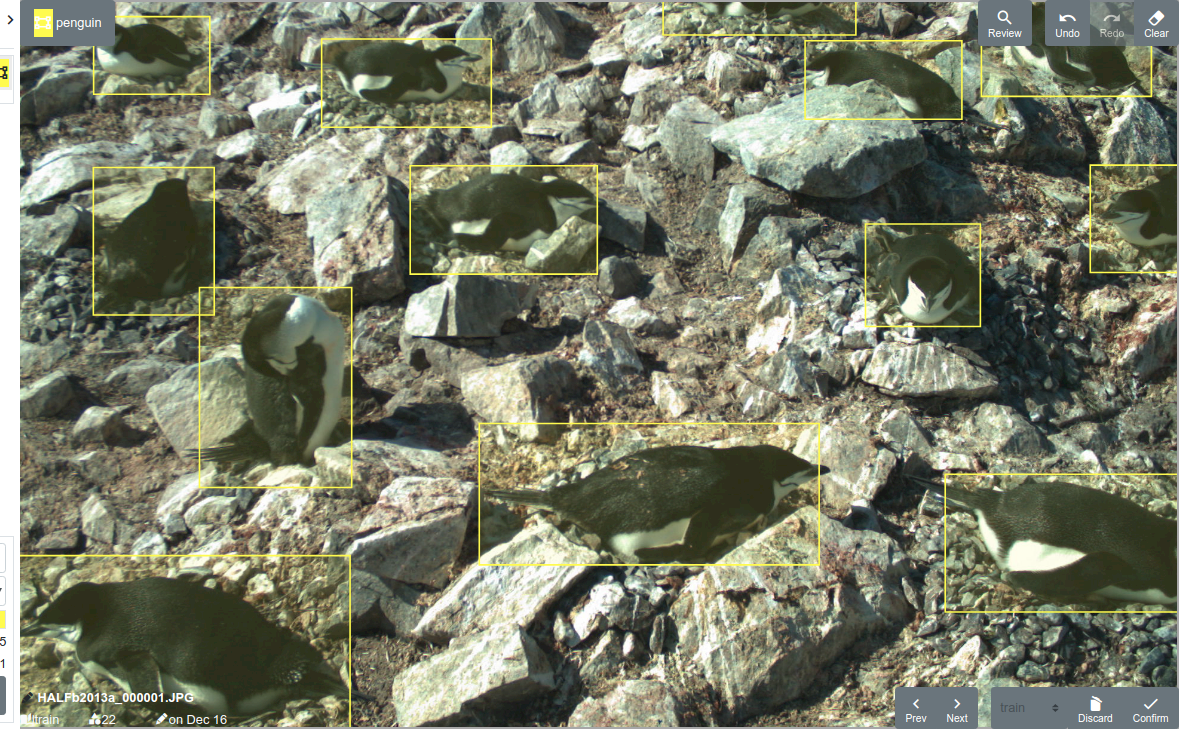
\includegraphics[width=1.0\linewidth]{figures/annotation/screenshots/penguins2.png}
   \caption{\emph{penguins}}
\end{subfigure}%
\begin{subfigure}[t]{0.24\linewidth}
  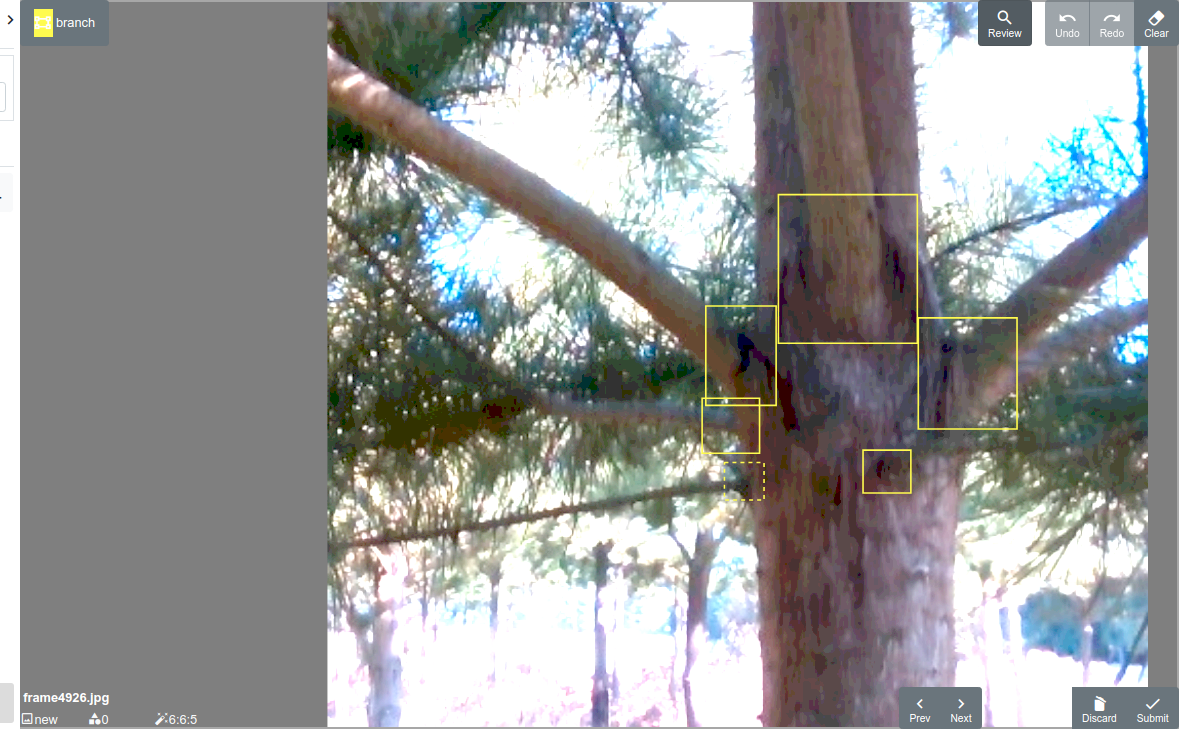
\includegraphics[width=1.0\linewidth]{figures/annotation/screenshots/branches3.png}
   \caption{\emph{branches}}
\end{subfigure}%
\begin{subfigure}[t]{0.24\linewidth}
  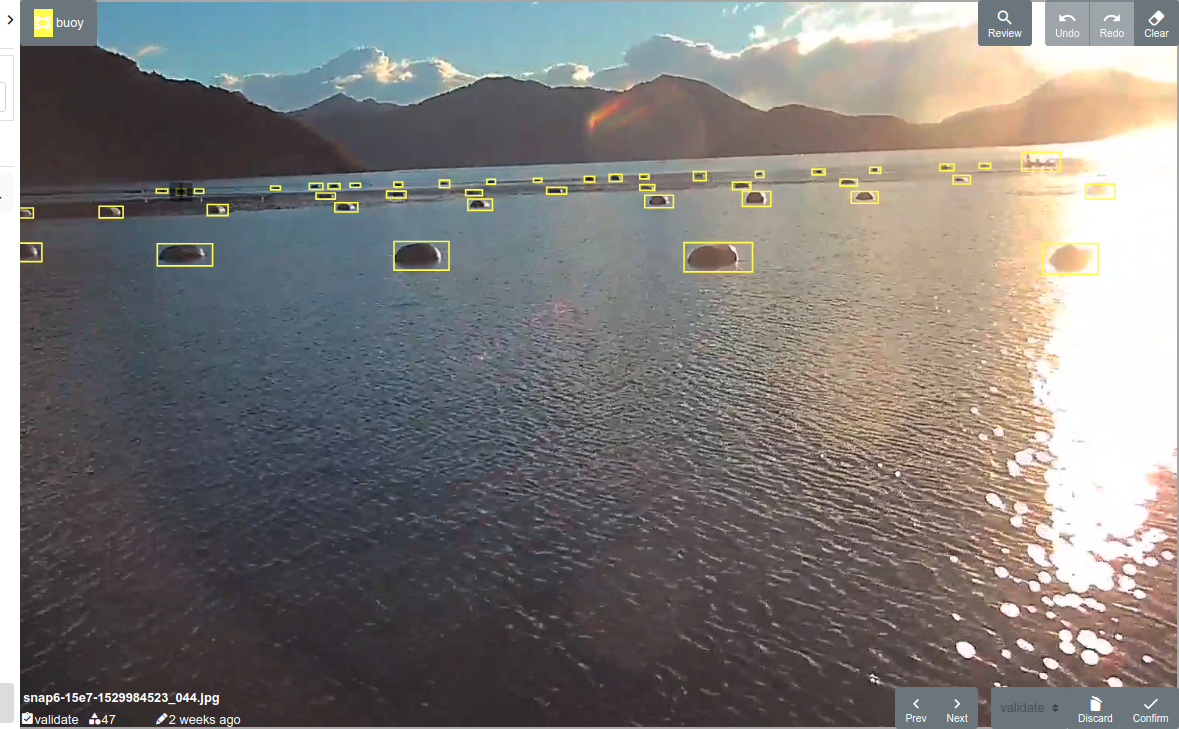
\includegraphics[width=1.0\linewidth]{figures/annotation/screenshots/buoys.png}
   \caption{\emph{buoys}}
 \end{subfigure}
\begin{subfigure}[t]{0.24\linewidth}
  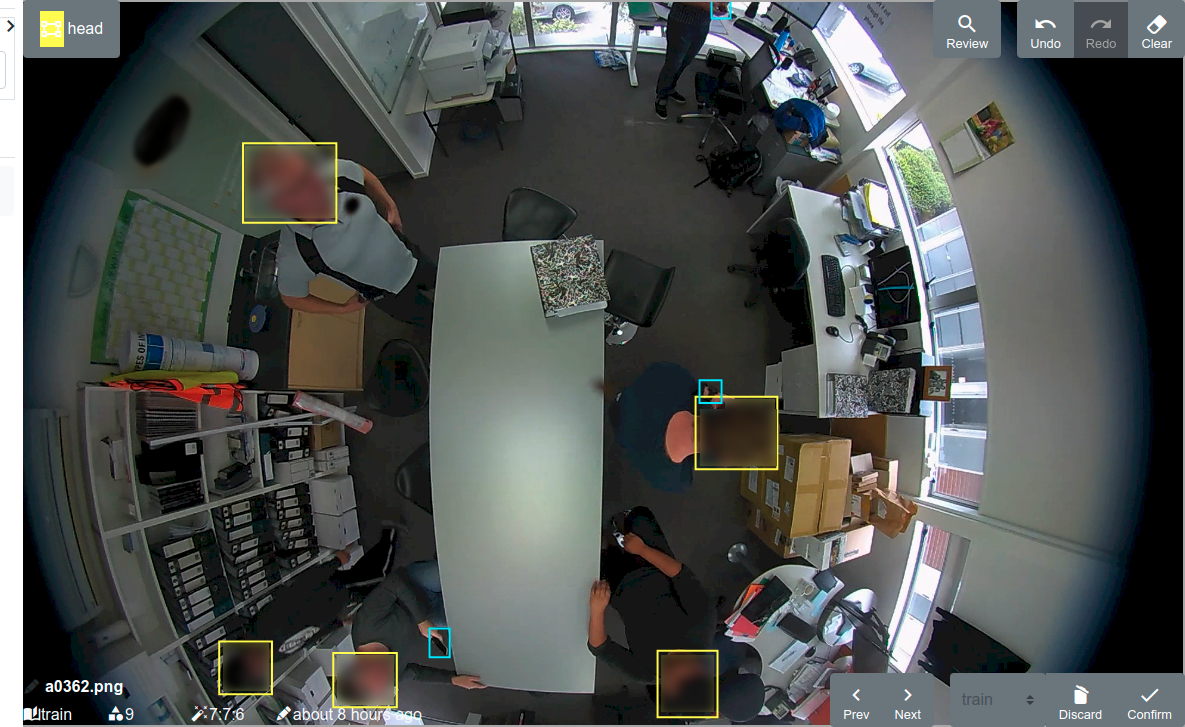
\includegraphics[width=1.0\linewidth]{figures/annotation/screenshots/victor.png}
  \caption{\emph{fisheye}}
\end{subfigure}%

\begin{subfigure}[t]{0.24\linewidth}
  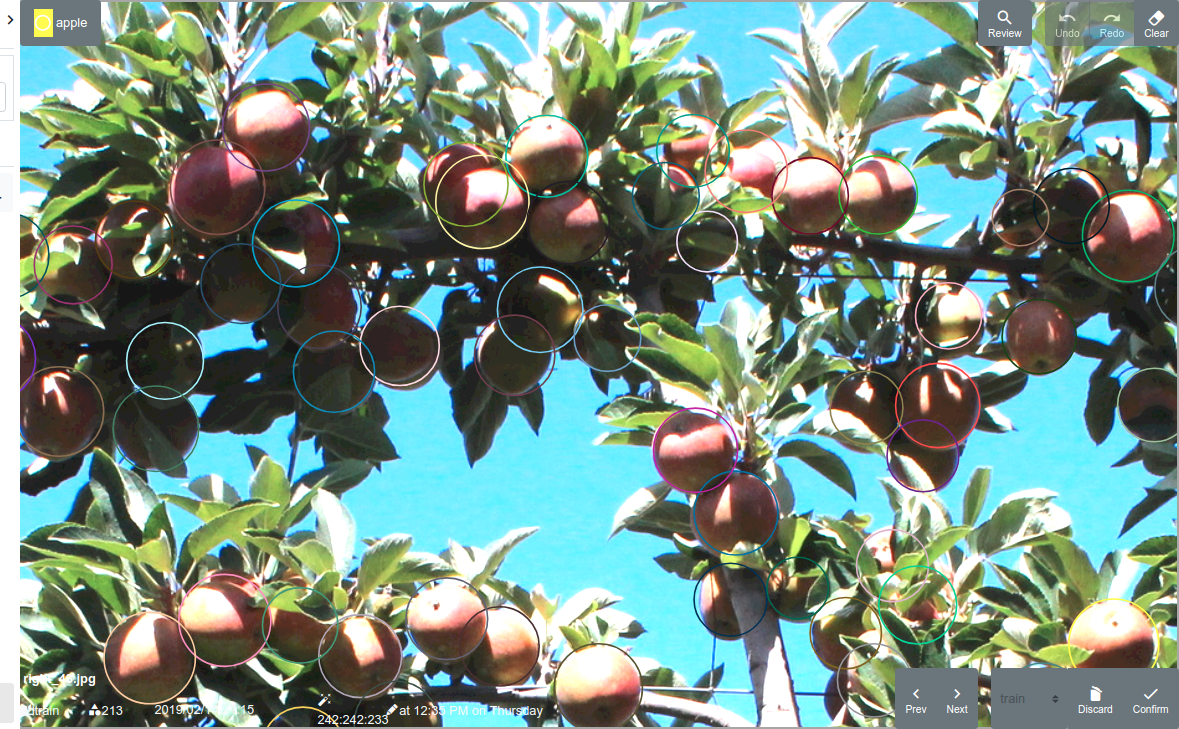
\includegraphics[width=1.0\linewidth]{figures/annotation/screenshots/apples_big2.png}
  \caption{$\mathrm{apples_1}$}
\end{subfigure}%
\begin{subfigure}[t]{0.24\linewidth}
  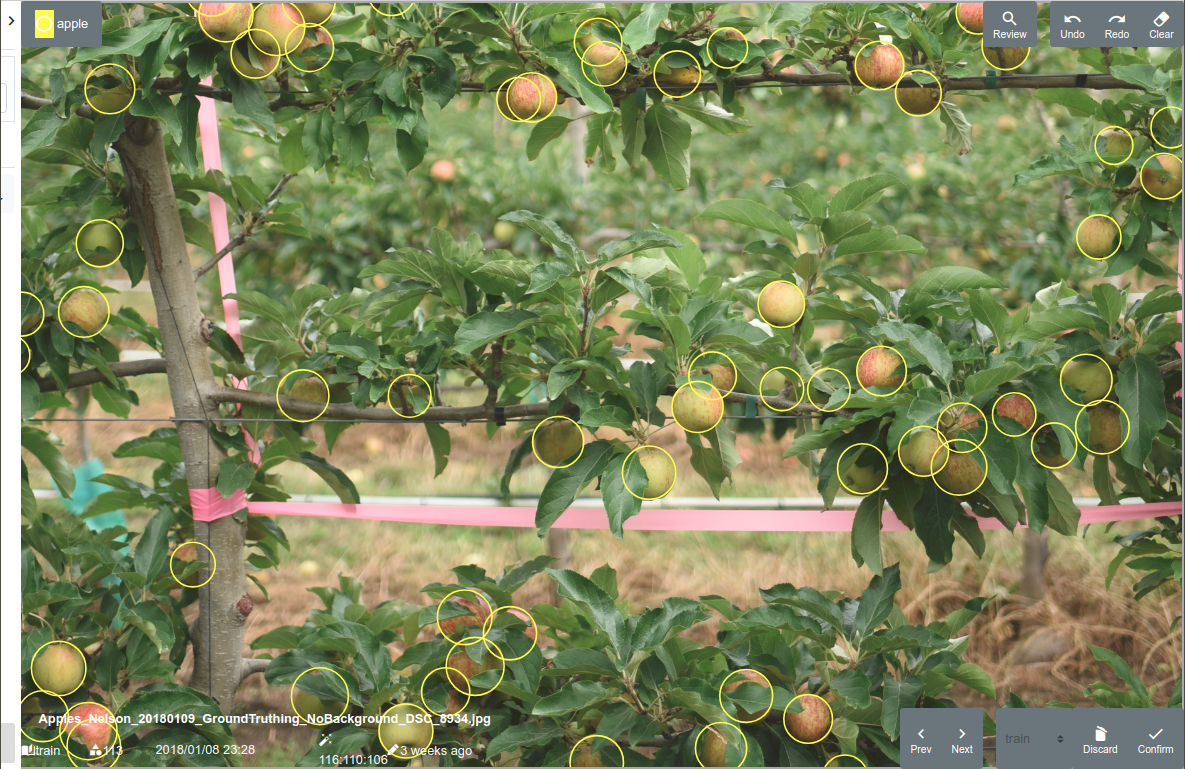
\includegraphics[width=1.0\linewidth]{figures/annotation/screenshots/apples2.png}
  \caption{$\mathrm{apples_2}$}
\end{subfigure}%
 \begin{subfigure}[t]{0.24\linewidth}
  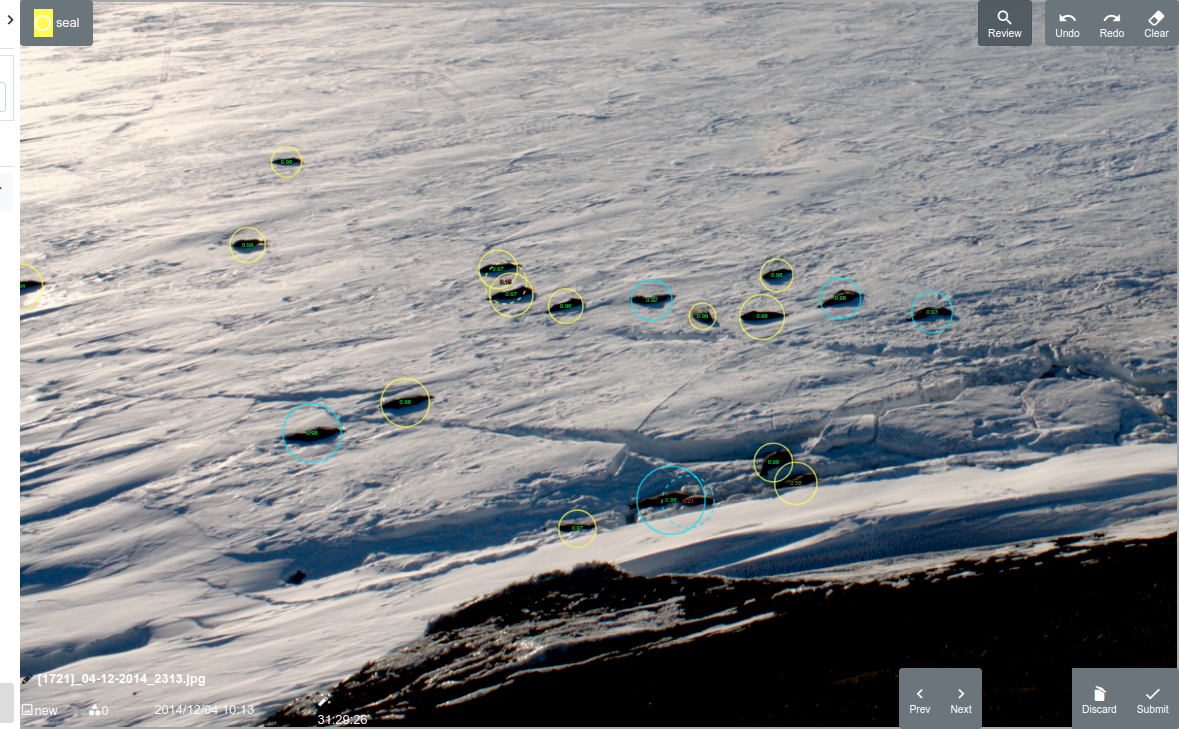
\includegraphics[width=1.0\linewidth]{figures/annotation/screenshots/seals_small2.png}
  \caption{\emph{seals}}
\end{subfigure}%
\begin{subfigure}[t]{0.24\linewidth}
  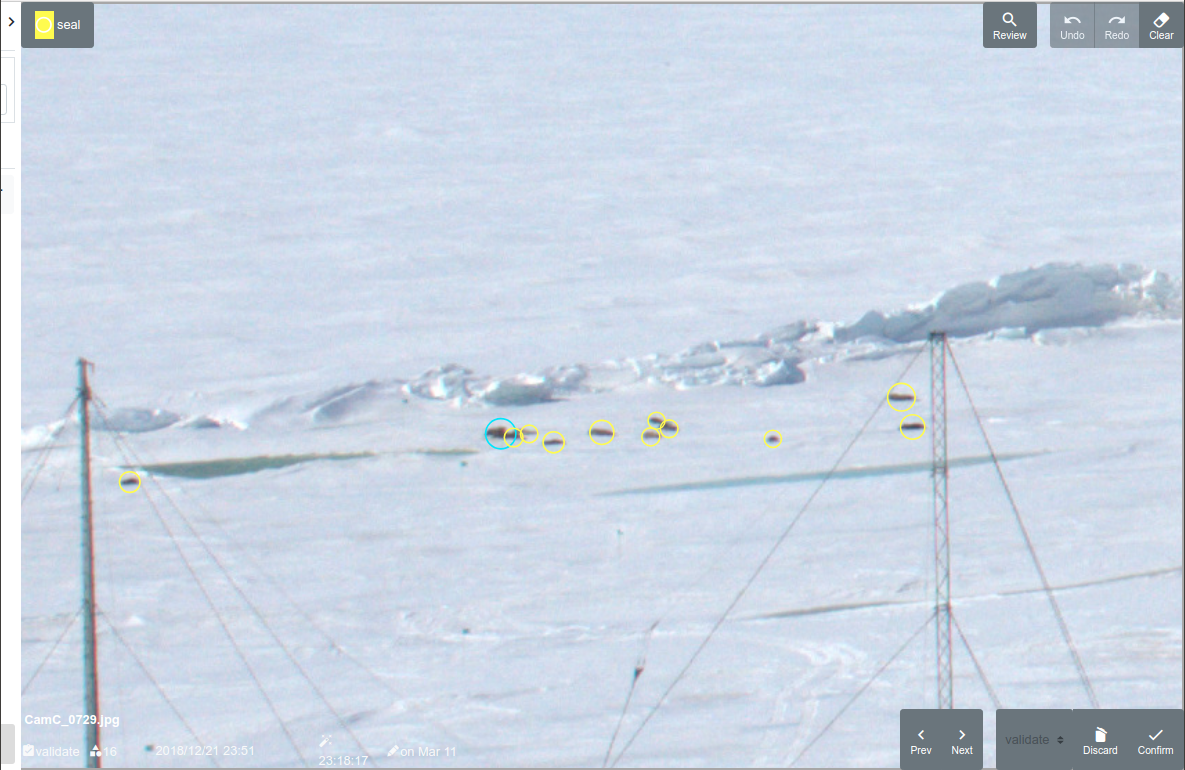
\includegraphics[width=1.0\linewidth]{figures/annotation/screenshots/scott_base_sunny.png}
  \caption{\emph{scott base}}
\end{subfigure}
\begin{subfigure}[t]{0.24\linewidth}
  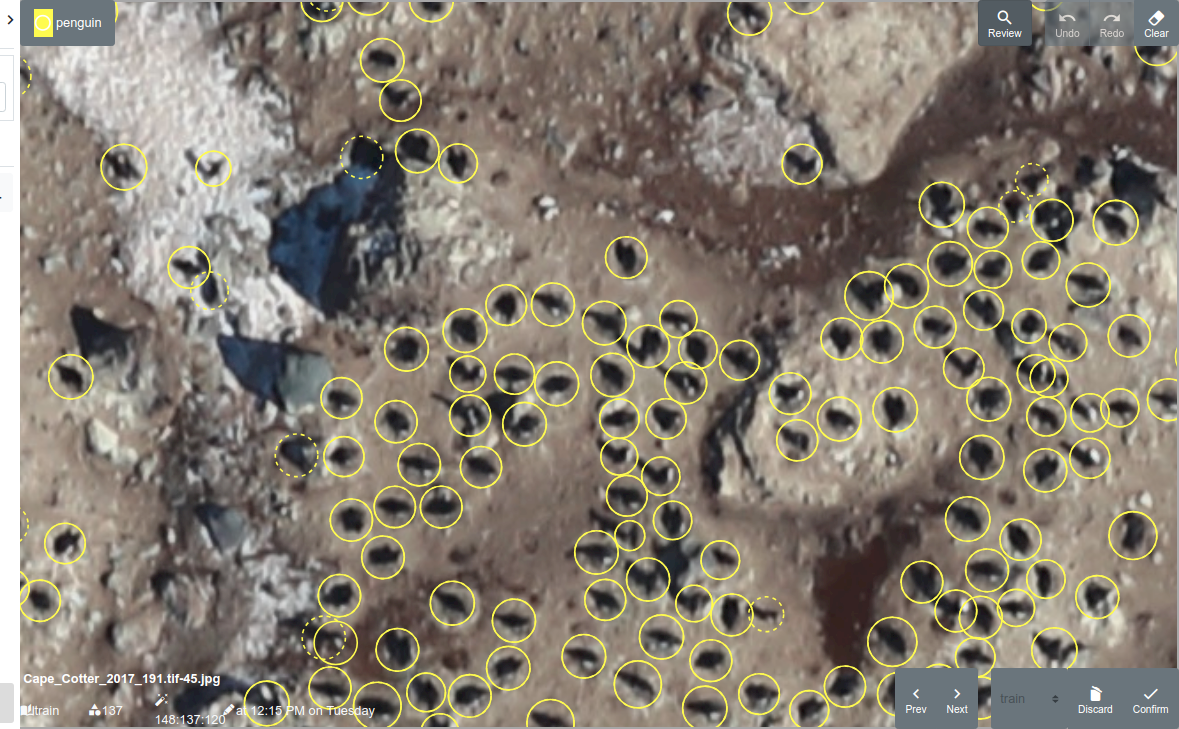
\includegraphics[width=1.0\linewidth]{figures/annotation/screenshots/penguins_aerial2.png}
  \caption{\emph{penguin survey}}
\end{subfigure}%
\begin{subfigure}[t]{0.24\linewidth}
  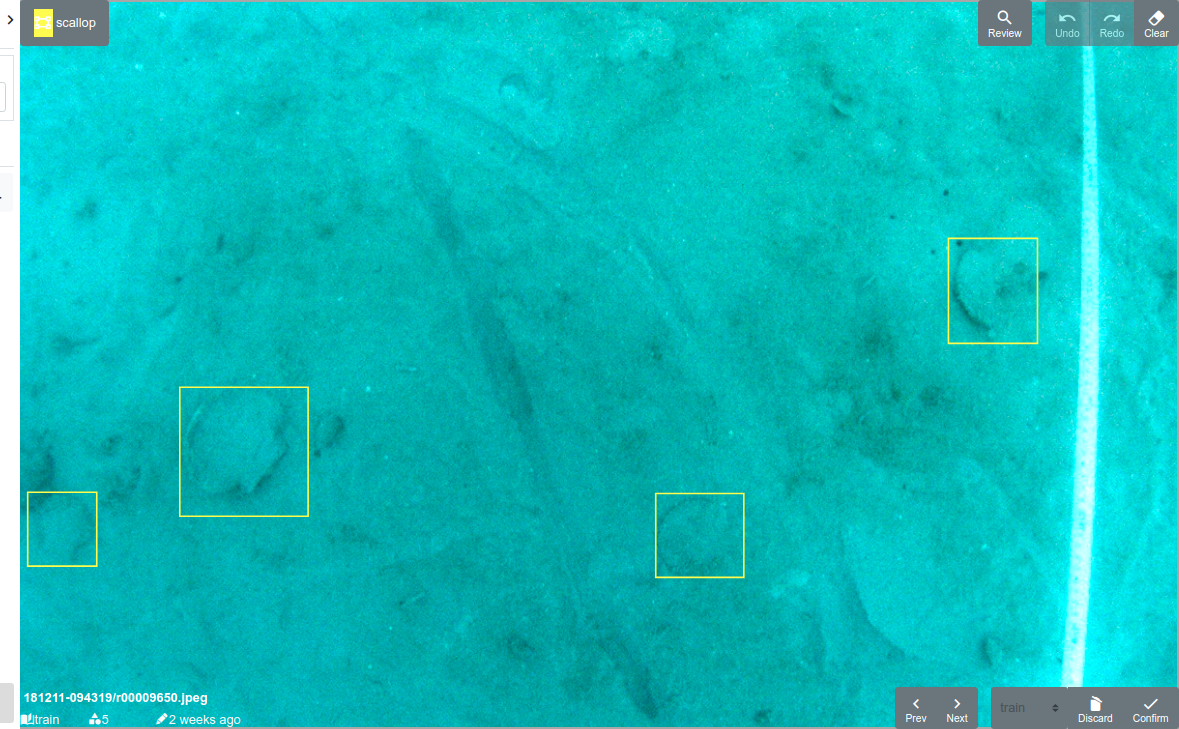
\includegraphics[width=1.0\linewidth]{figures/annotation/screenshots/scallops4.png}
  \caption{\emph{scallops}}
\end{subfigure}
\caption{Representative images of datasets (and annotations) annotated in this work}
\label{fig:datasets_all}
\end{figure}


In this chapter I present the results of an exploratory study, and demonstrate the practical use of the \gls{VBA} based annotation tool by annotating 10 image sets (several of them twice) on a variety of object detection tasks. Representative images are shown in figure~\ref{fig:datasets_all}. I analyse how the performance of the object detector changes as annotation progresses, with respect to the number and type of corrections required.

\section{Image sets and datasets}


The datasets comprise of firstly, a mix of relatively small scale image sets annotated for the sake of evaluating and developing the annotation method, and secondly, preliminary datasets as trial runs for larger scale annotation. A number also are annotated for a niche application, which seems suited to this kind of annotation method, in counting wildlife. Continuous annotation time (as defined below) was between approximately an hour for the smallest sets and up to eight hours for the largest.

\begin{threeparttable}[phtb]
\label{tab:resolutions}
\centering
\caption{Overview of datasets: number (n) and size of annotation, number and size of image.  } 
\begin{tabular}{lllllll}
dataset & n & images & box length & image size & \shortstack{training \\ crop} & \shortstack{validation \\ $AP_{COCO}$} \\
\toprule
$penguins$        & 7473        & 306    & $255 \pm 118$   &  $2048\times1536$  & 800                                   & 75.9                   \\
$branches$        & 2249        & 451    & $41.5 \pm 13.9$ &  $400\times400$    & 320                                   & 62.6                   \\
$seals$           & 4351        & 240    & $68.7 \pm 20.8$ &  $3920\times1600$  & 1024                                    & 80.7                   \\
$seals_b$         & 1256        & 82     & $63.4 \pm 17$   & $3920\times1600$  & 1024                                                     & 72.9        \\
$scott\:base$     & 7759        & 301    & $15 \pm 3.21$     & \shortstack[l]{$3927\times500$ -- \\ $5200\times700$} & 400  & 81.4  \\
$apples^1$        & 21637       & 300    & $78.4 \pm 14.9$ &  $2592\times1728$ & 1024 & 51.8                   \\
$apples^2$        & 13418       & 168    & $92.8 \pm 11.9$ &  $3008\times2008$  & 1024                                    & 74.5                   \\
$scallops_e$      & 3669        & 6741   & $114 \pm 40.2$  &  $1280\times1024$  & 800                                   & 65.0                   \\
$fisheye$         & 2598        & 367    & $96.6 \pm 32.7$ &  $2048\times1944$ & 1024                                     & 78.9                   \\
$buoys_d$         & 7221        & 207    & $38.9 \pm 42.8$ &  $1920\times1080$ & 600                                    & 70.9                   \\
\shortstack{$penguin$ \\ $survey$} & 13210       & 352    & $22.6 \pm 2.11$ & \shortstack[l] {$406\times405$ -- \\ $672\times448$} & 400  & 61.6               \\ 
\bottomrule
\end{tabular}
\begin{tablenotes}
\small
\item $*$ Subscripts denote different annotator, for example $seals_b$ is annotated by annotator $b$ where images from the same image set (not necessarily the same ones) are annotated by different users.  
\item $\ddagger$ Superscript denotes images from a different distribution of images
\item Datasets specified without subscript are annotated by the author.
\item $\dagger$ A bug relating to anchor box positioning impacted object detection. 
\end{tablenotes}
\end{threeparttable}


\subsection{penguins}
An image set used in the development of the annotation tool, primarily because the object detector performed well on the images after only a few annotated images and because of the relative uniformity of the images. The images used are a subset 'HALFb'  of the Penguin dataset \cite{PenguinData}, used for counting, using point annotations \cite{Arteta2016}. 
\subsection{$branches$}
An image set annotated as a test run for cut-point detection, where branch intersections (including hidden ones) are annotated with boxes by including the collar of the branch and a piece of the branch. Images are randomly sampled from a large set of frames extracted from several video sequences of orbits around trees. Images are lower resolution than other image sets ($ 320\times320 $ images), and a number of images have poor contrast.

\subsection{buoys}
An image set for monitoring mussel buoys. The ultimate idea is to monitor the growth of mussels by visually examining the height of the buoy out of the water, but this aspect is out of the scope of this work. Object detection is used as a first step however, and used to determine a water plane. Images are sampled from video sequences taken from a camera fixed to another mussel buoy. As a result the view angles are somewhat limited, but do change as the buoy (with the camera attached) rotates with the swell, with weather and lighting conditions also giving a variation to the appearance. 

Although image resolution is reasonably high ($1920\times1080$), there is a considerable number of visible artefacts from video compression. Buoys in the distance become very tiny, and were ignored once they became hard to distinguish. Buoys also tended to line up and occlude each other, so these buoys were also ignored.


\subsection{fisheye}
    
A test for detecting people (heads) and cellphones in roof mounted fisheye camera images. Trained models for human detection (and pose recognition) are readily available but fail on fisheye images because the orientation and scale of an object changes, dependent on their position in the image. Person detection worked almost immediately after a handful of images, with only minor corrections required, however, cellphone detection required more intervention, but began to work reliably towards the end of annotation. Experiments afterwards showed that the high-resolution ($2048\times1944$) was necessary to detect the cellphones; detection failed at half resolution.

\subsection{$\mathrm{apples^1}$}

A set of images of trellised apple trees with many apples per image. Only the apples in the foreground were annotated; small apples and cherries in the background provided distraction. Leaves occlude a large number of apples in the image set, however, all apples which could be located were annotated. Often, it is possible to guess quite accurately the location of the apple because a section of the curved outline can be seen, although it is harder to accurately guess the size of the apple. 

Images were taken with a high-resolution DSLR camera and scaled to half resolution ($2592\times1728$); apples in the photos at this resolution are large ($50$-- $200$ pixels, median $80$). Despite only annotating 300 images, this dataset has the most annotations (over $22000$) and took longest to annotate. Lighting was often less than ideal as direct sunlight caused poor contrast in many images.
    
\subsection{$\mathrm{apples^2}$}
    
Another set of images of trellised apple trees; when compared to \emph{$apples^1$}, has a higher degree of  photographic consistency (resulting in more consistent sizes and number of apples), and better focus on the foreground (less distracting background with some images, additionally, given a black backdrop). These differences manifested themselves in the difference in validation accuracy seen in table~\ref{tab:validation_corrections}, reaching a higher accuracy than \emph{$apples^1$}.

While at a similar resolution to \emph{$apples^1$}, some images were captured as portrait as well as landscape orientation, whereas all the images in \emph{$apples^1$} are landscape orientation. The same annotation strategy was used between both sets, to annotate all apples which can be localised.

\subsection{seals}
    
 A time series sequence of images taken as part of the \emph{Turtle Rock Seal Survey} \cite{Eisert2015}. The images are captured 10 minutes apart, taken of part of an Antarctic Weddell seal colony around Turtle Rock, an island approximately 12km north of Scott Base. The time period was a three week period from the 28th November to the 19th of December, 2014. The purpose of this monitoring is to establish haul-out patterns where seals sit on the ice (in order to avoid predation).  

Images were taken from a high-resolution DSLR camera and cropped to give a resolution of $3920\times1600$. The images were annotated twice. Different images were annotated in both cases, a result of random selection. Separate test sets, using the same images in both cases, were created before annotation began. From a set of $3000$ images, the first $240$ images were annotated by the author and the second $82$ by user $b$. The test set comprised $46$ images.

The seals generally sat well separated from each other and were very clearly distinct, except for mother and pup combinations who often sat right next to each other. Lighting was occasionally quite difficult for observations. Seals were annotated as two classes, either: (a) single seal or (b) mother next to pup.  The misclassification of mother and pup vs. single seal was the largest source of error during annotation and in validation. Disambiguation of the two is difficult for a human without viewing the images in the time series, where it becomes apparent due to the seal's movement.

More details can be found in section~\ref{sec:case_seals}.

\subsection{scott base}
    
Another time series sequence of images, part of the \emph{Weddell Seal Abundance Monitoring Programme} \cite{Eisert2019}. Images were captured 10 minutes apart, taken of Weddell seals around Scott Base, Antarctica. Two different views were used in this work (three views were captured, but the third view was not used as it contained few seals in the time period used here). The purpose is for population monitoring annually to be able to evaluate the impact on the seal population when Scott Base is renovated in the coming years. 

Two different DSLR cameras were used, each with a different viewpoint (and different image size). Images were cropped to the regions containing seals, as they were very wide, and $5000\times700$ from one viewpoint. The viewpoints, unlike the \emph{seals} images, were from far away and the seals were tiny (a mean of $15$ pixels diameter) with considerable blurriness.  
    
More details can be found in section~\ref{sec:case_seals}.
    
\subsection{penguin survey}
    
The images are from the Ad\'elie Penguin Census \cite{Lyver2014}, an aerial photographic survey (started in 1981 and continuing until the present) in which a complete census of the Ad\'elie penguin population is taken by counting nesting pairs. High-resolution photographs are taken from an altitude of 2000-2500 feet.

Three separate annotations are performed; two of them from images comprising part of two large colonies, and one from a distinct and much smaller colony in 3 separate images. In each case, the large images are broken into small images for practical reasons, including the number of annotations the software can handle, as well as the number of annotations which are  practical for an annotator to check in one go.
    
The images, once chopped into pieces, are relatively small, but still contain large numbers of penguins, comparable to $apples^2$ in terms of annotation per image (see figure~\ref{fig:instances_image_plot}). The penguins themselves are small and blurry, with two forms, either sitting or standing. These become  easily confused, and also difficult to distinguish from the shadows in rocky areas and are considerably ambiguous. 

\subsection{scallops}
    
These images are drawn from video frames taken by an underwater \gls{ROV} used to survey a small seabed area containing scallops. The images are unique from the others used in this work, in that the object instances are very sparse; there are many images with no scallops. 

The images are part of a project intending to survey scallops, and eventually develop methods of mechanically harvesting them. The usual current method of harvesting scallops is by dredging the sea floor, an environmentally destructive method. By harvesting scallops individually, the destruction of the sea floor can be avoided.

These images are an initial test run of both image capturing and annotation. The lighting on the \gls{ROV} went out mid capture, leading to approximately half the images appearing in good lighting and the other half in dim blue natural light. The point of view also changed mid capture, some images being forward facing, and others downward facing. The images often traversed backwards and forwards across the same areas, thus limiting the visual appearance (often seeing the same scallop repeatedly). 

The annotation of the scallops dataset was performed by a combination of two scallop experts. It was intended as a trial of example selection, and was initially configured to select images in order of highest detection count (done by the first annotator). However, after approximately $120$ minutes ($25\%$ of the time), a second annotator took over and annotated the rest of the frames in sequence. 

The annotation criteria was that to be annotated, the scallop must be clearly visually alive; due to the turbidity of the sea water this meant that scallops are more uncertain further from the camera. Due to the criteria for annotation, this meant that often the same scallop was marked as positive in one frame and negative in the next. 

Training the object detector on the scallop dataset was more unstable in validation accuracy than other datasets annotated here (see figure~\ref{fig:datasets_lr} and figure~\ref{fig:scatter_loss_ap}). Given the differences between visual appearance in the source images (for example those with artificial light and those with natural light), combined with the discontinuous annotation criteria, it seems this is likely to blame for the apparent instability seen in training. 

In future, the plan for a larger scale annotation involves annotating scallops with a range of uncertainty, where the criteria is not \emph{scallop} or \emph{not scallop}, but \emph{scallop} with a degree of uncertainty, and only \emph{not scallop} when the object in question is definitely not a scallop. The sparseness of the scallop instances makes image selection relatively much more important; this is apparent when examining user actions in figure~\ref{fig:actions_dataset_b}, where it can be seen that the most common action by far is to \emph{submit} an image.



\begin{table}[]
\centering
\caption{ Statistics of user actions over annotations (anns.) of different datasets }
\label{tab:annotation_table}
\begin{tabular}{llllll}
dataset           & actions & anns. & \shortstack {ann. time \\ (minutes)} & \shortstack{instances \\ per minute} & \shortstack{actions \\ per ann.} \\
\toprule
$penguins$        & 2,070   & 7473        & 140                       & 53.5                 & 0.28                   \\
$branches$        & 745     & 2249        & 63                        & 35.7                 & 0.33                   \\
$seals$           & 587     & 4351        & 89.8                      & 48.5                 & 0.13                   \\
$seals_b$         & 453     & 1256        & 76.4                      & 16.4                 & 0.36                   \\
$scott\:base$     & 1,499   & 7759        & 123                       & 63.1                 & 0.19                   \\
$apples^1$        & 5,542   & 21637       & 511                       & 42.4                 & 0.26                   \\
$apples^2$        & 3,710   & 13418       & 364                       & 36.9                 & 0.28                   \\
$scallops_e$      & 2,065   & 3669        & 561                       & 6.54                 & 0.56                   \\
$fisheye$         & 337     & 2598        & 58.4                      & 44.5                 & 0.13                   \\
$buoys_d$         & 1,230   & 7221        & 234                       & 30.9                 & 0.17                   \\
$penguin\:survey$ & 1,616   & 13210       & 120                       & 110                  & 0.12                  \\
\bottomrule
\end{tabular}
\end{table}



\section {Evaluation methods}
\label{sec:ann_evaluation}

The primary method of evaluation used in this work is that of \emph{continuous testing}, whereby it is possible to characterise how the annotation process changes over time; how the model's predictions impact on the actions taken by the annotator, the type of actions and time required, and the accuracy of the model's predictions.

User edits are logged, along with predictions provided by the model (the starting point for annotating each image), and the final set of annotations submitted by the user. The accuracy of detections are verified directly by the user, giving continuous testing of the model predictions on unseen images as they're annotated.

The types of actions as well as the timing can provide useful cues as to the difficulty of the task, and the level of assistance provided by the object detection model. I break down these actions, and the relation of the actions to the original set of detections to the performance of the object detector in a few different ways: categorise the action types and frequencies; categorise the corrections applied to each annotation; and lastly use a locally weighted \gls{AP} to quantify object detection performance on newly annotated images.

\subsection{User actions}

The various user actions are discussed in section~\ref{sec:user_interface} in more detail. For the purposes of this chapter the user actions are broken down into categories:

\begin{itemize}
    \item {\bf transform}: an annotation is transformed (scaling, translation, corner dragged).
    \item {\bf confirm}: a weak detection is confirmed. This may also include a transformation of bounding box, but it is performed as one action.
    \item {\bf delete}: one or more annotations are deleted.
    \item {\bf add}: a new annotation is added.
    \item {\bf set class}: the class of an annotation is changed.    
    \item {\bf submit}: an image is submitted.    
\end{itemize}

\subsection{Annotation corrections}
\label{sec:corrections}

Another way of analysing the annotation process is to categorise each annotation by the nature of corrections applied to the original machine prediction (or lack of). This differs from user actions because: (a) multiple actions may be performed on one annotation, for example, a scaling and a translation, or changing the class and translation and (b) one action may modify multiple annotations, frequently a deletion of multiple false positives at once.

The following definitions are used:

\begin{itemize}
    \item {\bf positive}: a high confidence detection unchanged after verification.
    \item {\bf modified}: high confidence detection where either the box annotation or the class label has been modified.
    \item {\bf weak positive}: a weakly confident detection confirmed using the review mode (and potentially transformed).    
    \item {\bf false negative}: an object which was missed by the object detector and annotated manually by the user.    
    \item {\bf false positive}: an incorrect high confidence detection deleted by the user.
\end{itemize}

\subsection{Measuring progress with Cumulative Annotation Time}
\label{sec:ann_time}

\begin{figure}[ht!] 
\centering
  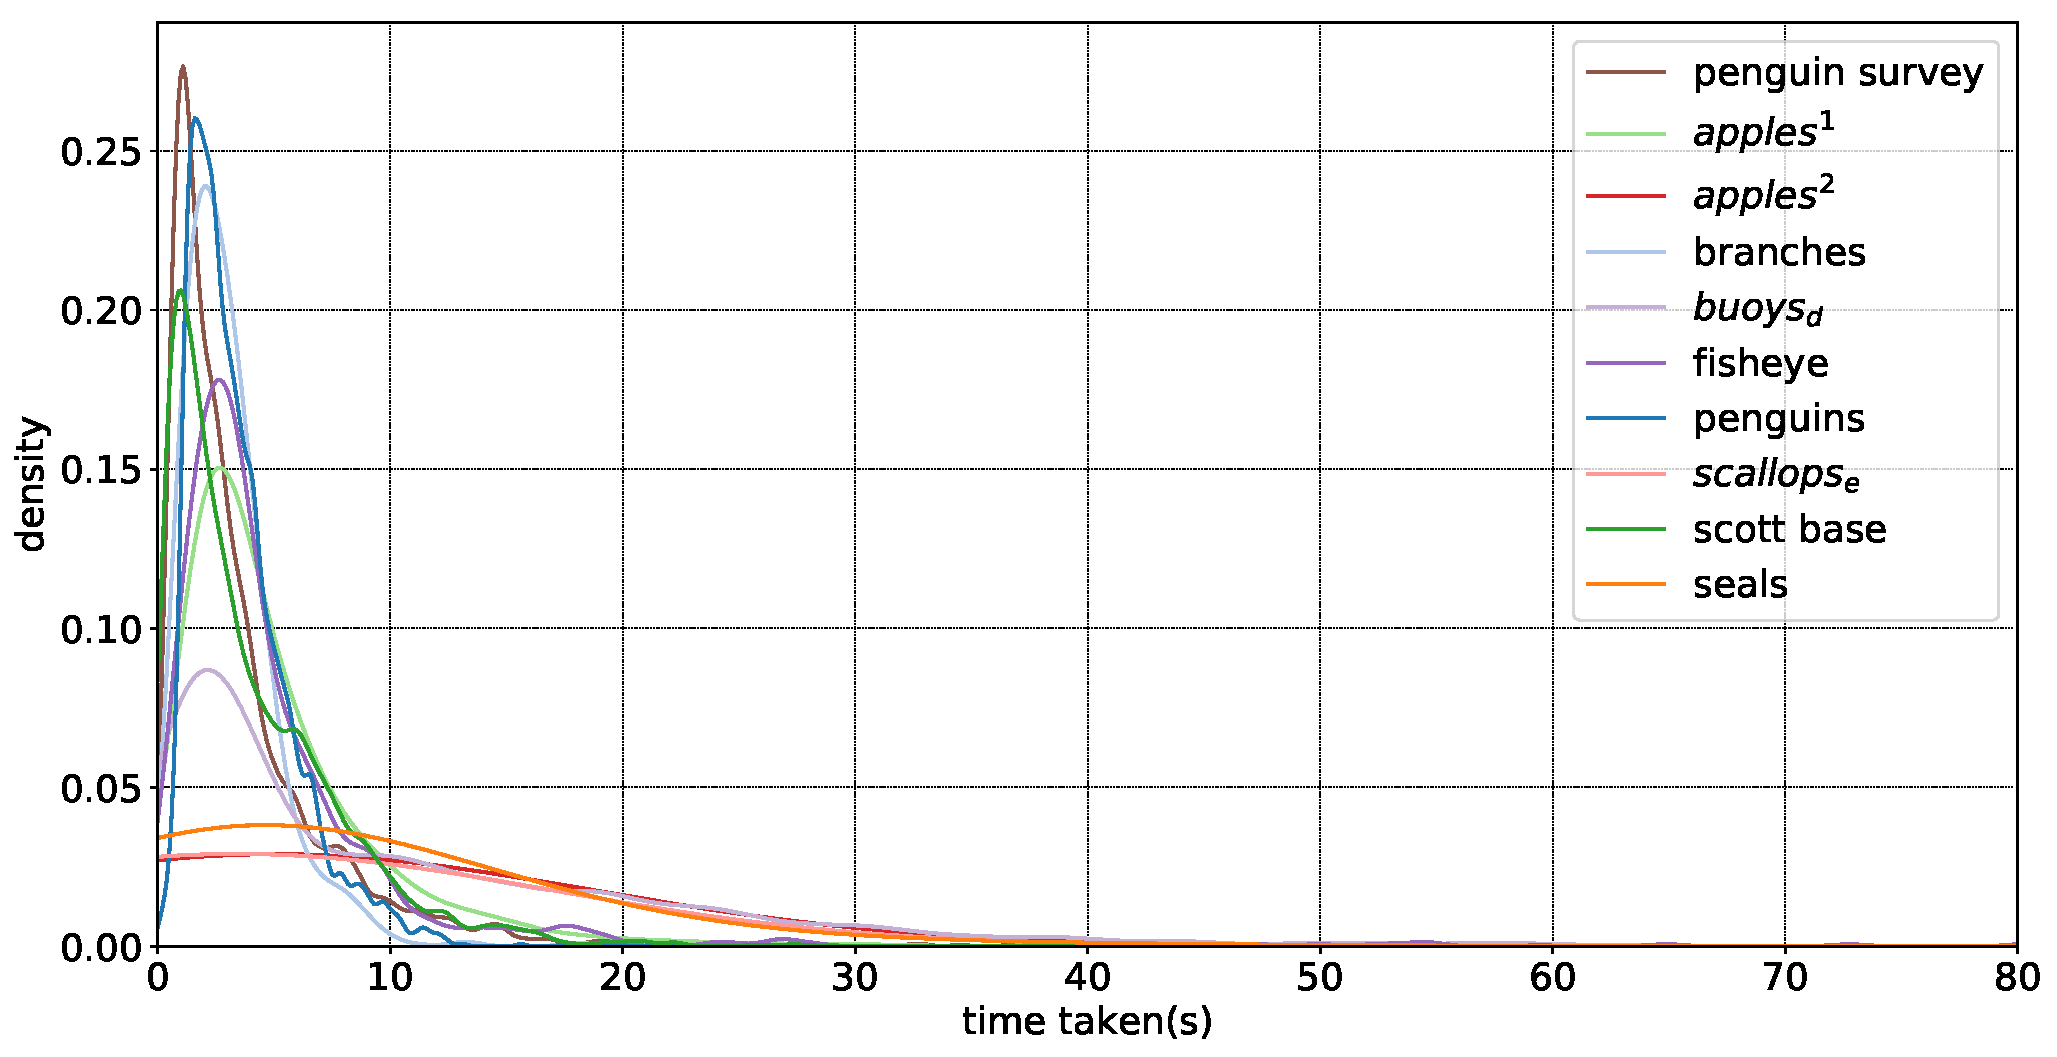
\includegraphics[width=1.0\linewidth]{charts/summaries/time_density.pdf}
  \caption{Time per action distributions for different dataset annotations}
  \label{fig:annotation_time_density}
\end{figure}

There are several ways progress could be measured in terms of annotation progress, such as the time spent since annotation began, the number of images or annotations submitted or \gls{CAT}, which we use in analysis for this chapter, which is the total time the user has spent actively using the tool.
 
In section~\ref{sec:schedule}, experiments in incrementally training on a dataset validation accuracy to be strongly dependent on the number of examples used. Annotation in general takes longer than training, and extra training without extra annotation generally has no positive effect.

For the above reason I use annotation time as opposed to training time, to measure and visualise the annotation progress. These assumptions  may change depending on the difficulty of the problem, complexity of a model or with many annotators contributing.



\subsection {Breaks in annotation}
\label{sec:break_detection}

The annotation logs recorded in this chapter were not taken in a controlled experimental setting, although an effort was made to be consistent in datasets annotated by the author. Datasets annotated by others can be seen to have more variability. It was therefore necessary to detect breaks where annotation was paused mid-image. Any action was capped at a maximum of one minute for this purpose. Ideally this would have been detected directly in the tool by detecting lack of input or loss of focus, and future studies will take this approach. 

Figure~\ref{fig:annotation_time_density} shows the distribution of times per action for different annotation efforts where any action taking more than a minute is a significant outlier in most cases. An obvious discrepancy can be seen between the \emph{scott base}, \emph{seals} and \emph{scallops} datasets, this is because the video sequences are useful in resolving ambiguity and more time is spent looking forward and backward at previous frames.

\subsection{Visualisation}
\label{sec:visualisation}

In order to visualise trends in the user action types, a fixed size density estimation is used with a gaussian kernel, $\sigma=5 minutes$. This approach is taken for both user actions, annotation correction types, the rate of annotations and using a weighted \gls{AP} to quantify overall detector performance at a particular point in  time.

Annotation actions, and corrected annotation types are all deemed to occur at the \gls{CAT} the image is submitted. Even though actions occurred at distinct points during an image annotation, the interest is in overall trends rather than particular trends within annotating each image. 

\subsection {Locally weighted Average Precision}
\label{sec:noisy_trends}

To give a single metric for object detection performance, where parts of a dataset are more important than others, I use a weighted \gls{AP}. The object detector's predictions are compared against the user's final annotations. A standard matching procedure is performed for all images (as opposed to tracking the user edits as in section~\ref{sec:corrections}).

In order to align with user actions across \gls{CAT}, a locally weighted \gls{AP} is used. To evaluate the locally weighted \gls{AP} at a particular point in cumulative annotation time, each image is given a weight according to its time difference from the image \gls{CAT}. As above, the gaussian kernel with $\sigma=5 minutes$ is used.

Annotations in each image are weighted by the image weight for the purposes of counting false positive, false negative and true positive counts. From there, weighted precision and recall and \gls{AP} are computed exactly as normal (see section~\ref{sec:evaluation_metrics}).


\section {Dataset overview}
\subsection {Size distribution}

\begin{figure}[ht]
\centering
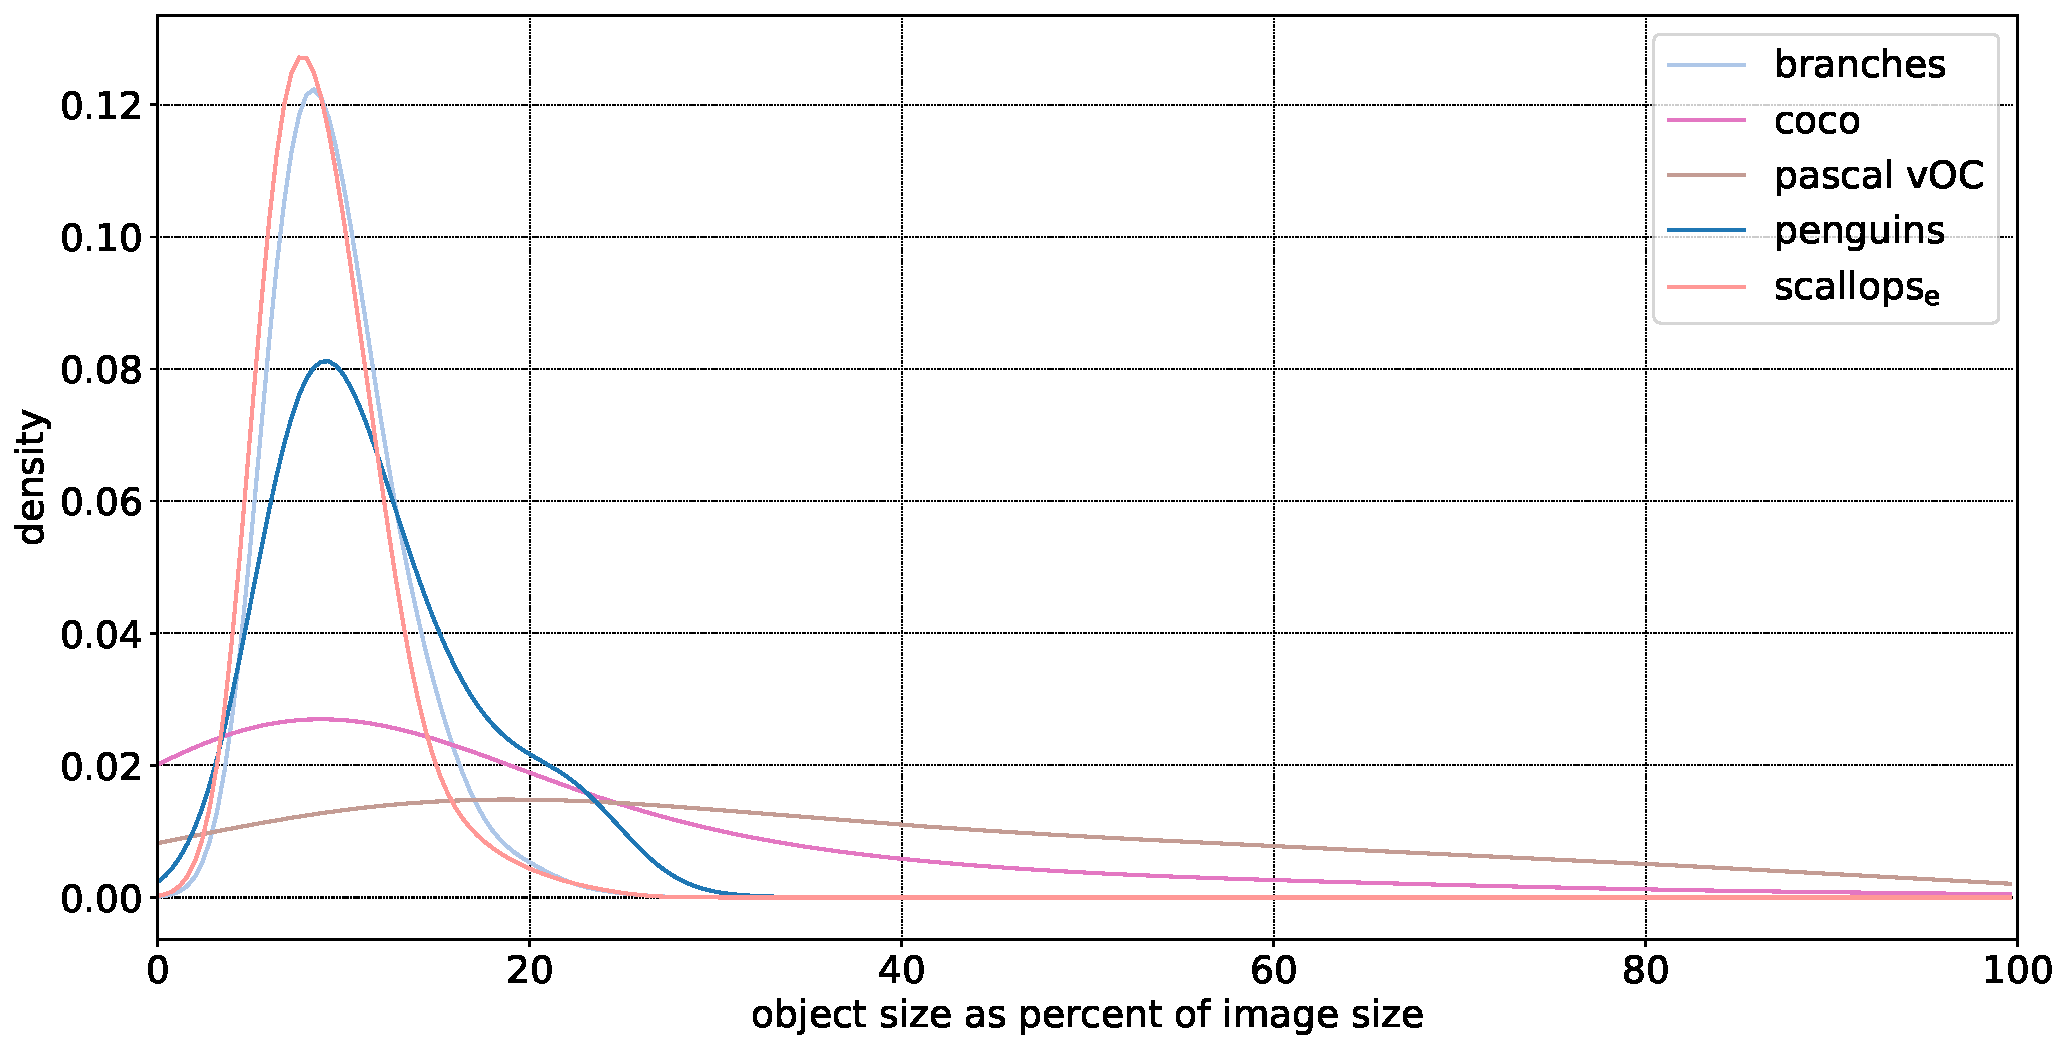
\includegraphics[width=1.0\linewidth]{charts/summaries/sizes_density.pdf}
\caption{Object bounding box size distributions as percentage of the object size to the image size (average of width and height) }
\label{fig:box_sizes}
\end{figure}
 

\begin{figure}[ht]
\centering
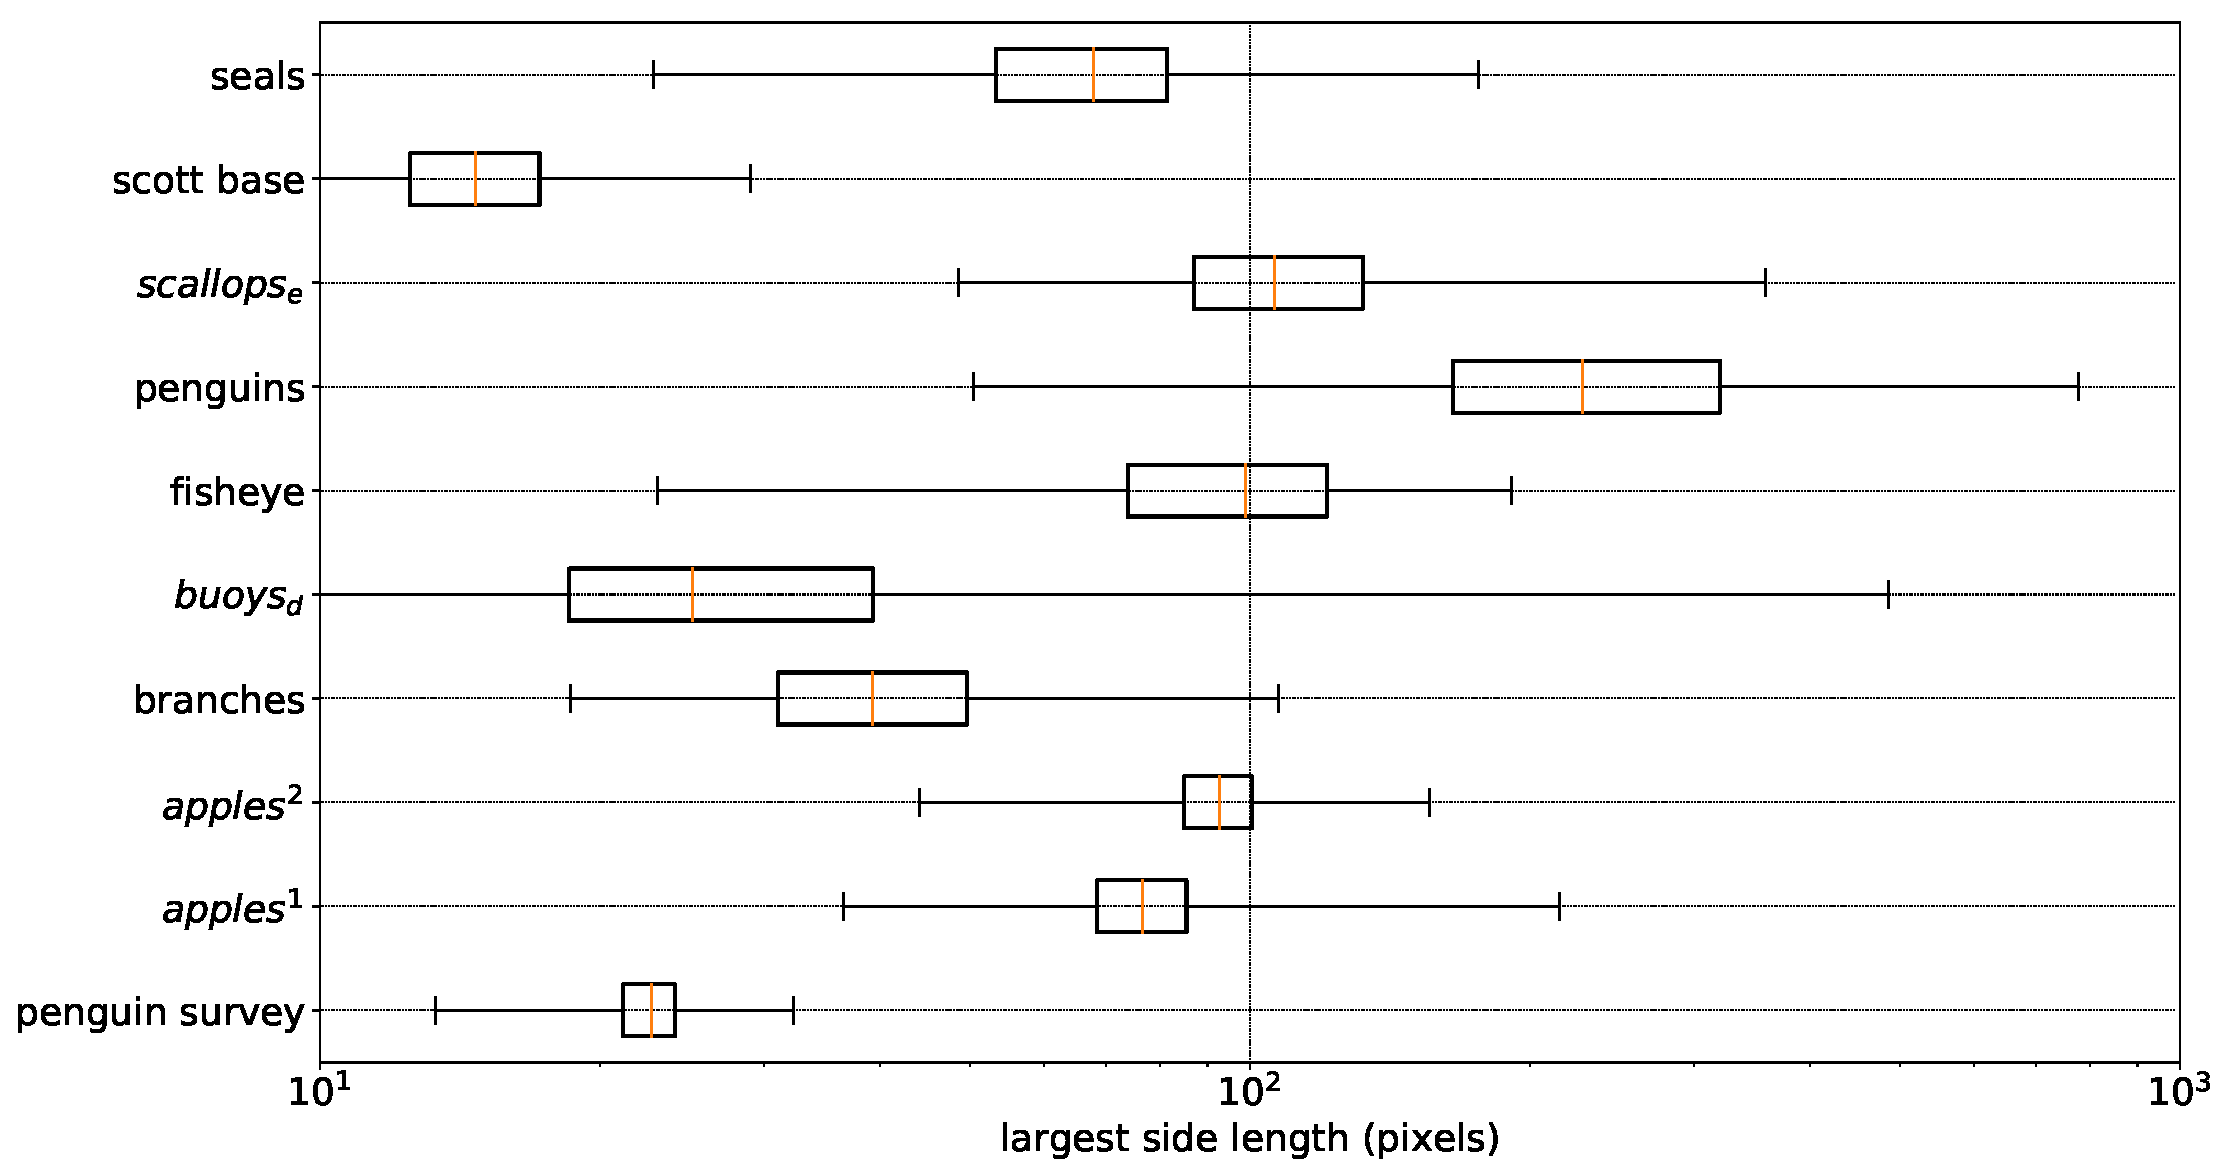
\includegraphics[width=1.0\linewidth]{charts/summaries/sizes_boxplot.pdf}
\caption{ Distribution of object box sizes in pixels for all datasets. Box plot showing quartiles, range and median (red line) on a log scale. Size here is measured as the larger side length in pixels. }
\label{fig:box_sizes_plot}
\end{figure}

The sizes of objects in these datasets, in general, are small compared to more mainstream object detection datasets. This can be seen in figure~\ref{fig:box_sizes}, where compared to the Pascal VOC \cite{Everingham2008}, or COCO \cite{Lin2014}, the box sizes are smaller compared to the image size and less widely distributed. 

Figure~\ref{fig:box_sizes_plot}  shows the distribution of object sizes (in pixels) of all the datasets together for comparison. In particular, the \emph{penguin survey} and \emph{scott base} datasets have particularly tiny objects.

It can be seen that although the box sizes are relatively small, compared to the image, that for high-resolution images the objects can still be relatively large in pixels.

Two different types of annotations are used in the annotations of these datasets. Circular annotations are used for very small objects and for counting objects where precise localisation is of less concern; circular annotations are also used for apples, where it just happens to match the object shape well. The difference to the object detector is that a centre and radius is estimated (instead of centre, width and height). The circles are treated as a square for computations such as \gls{IOU} overlap.

\subsection {Instance distribution}

\begin{figure}[ht!]
\centering
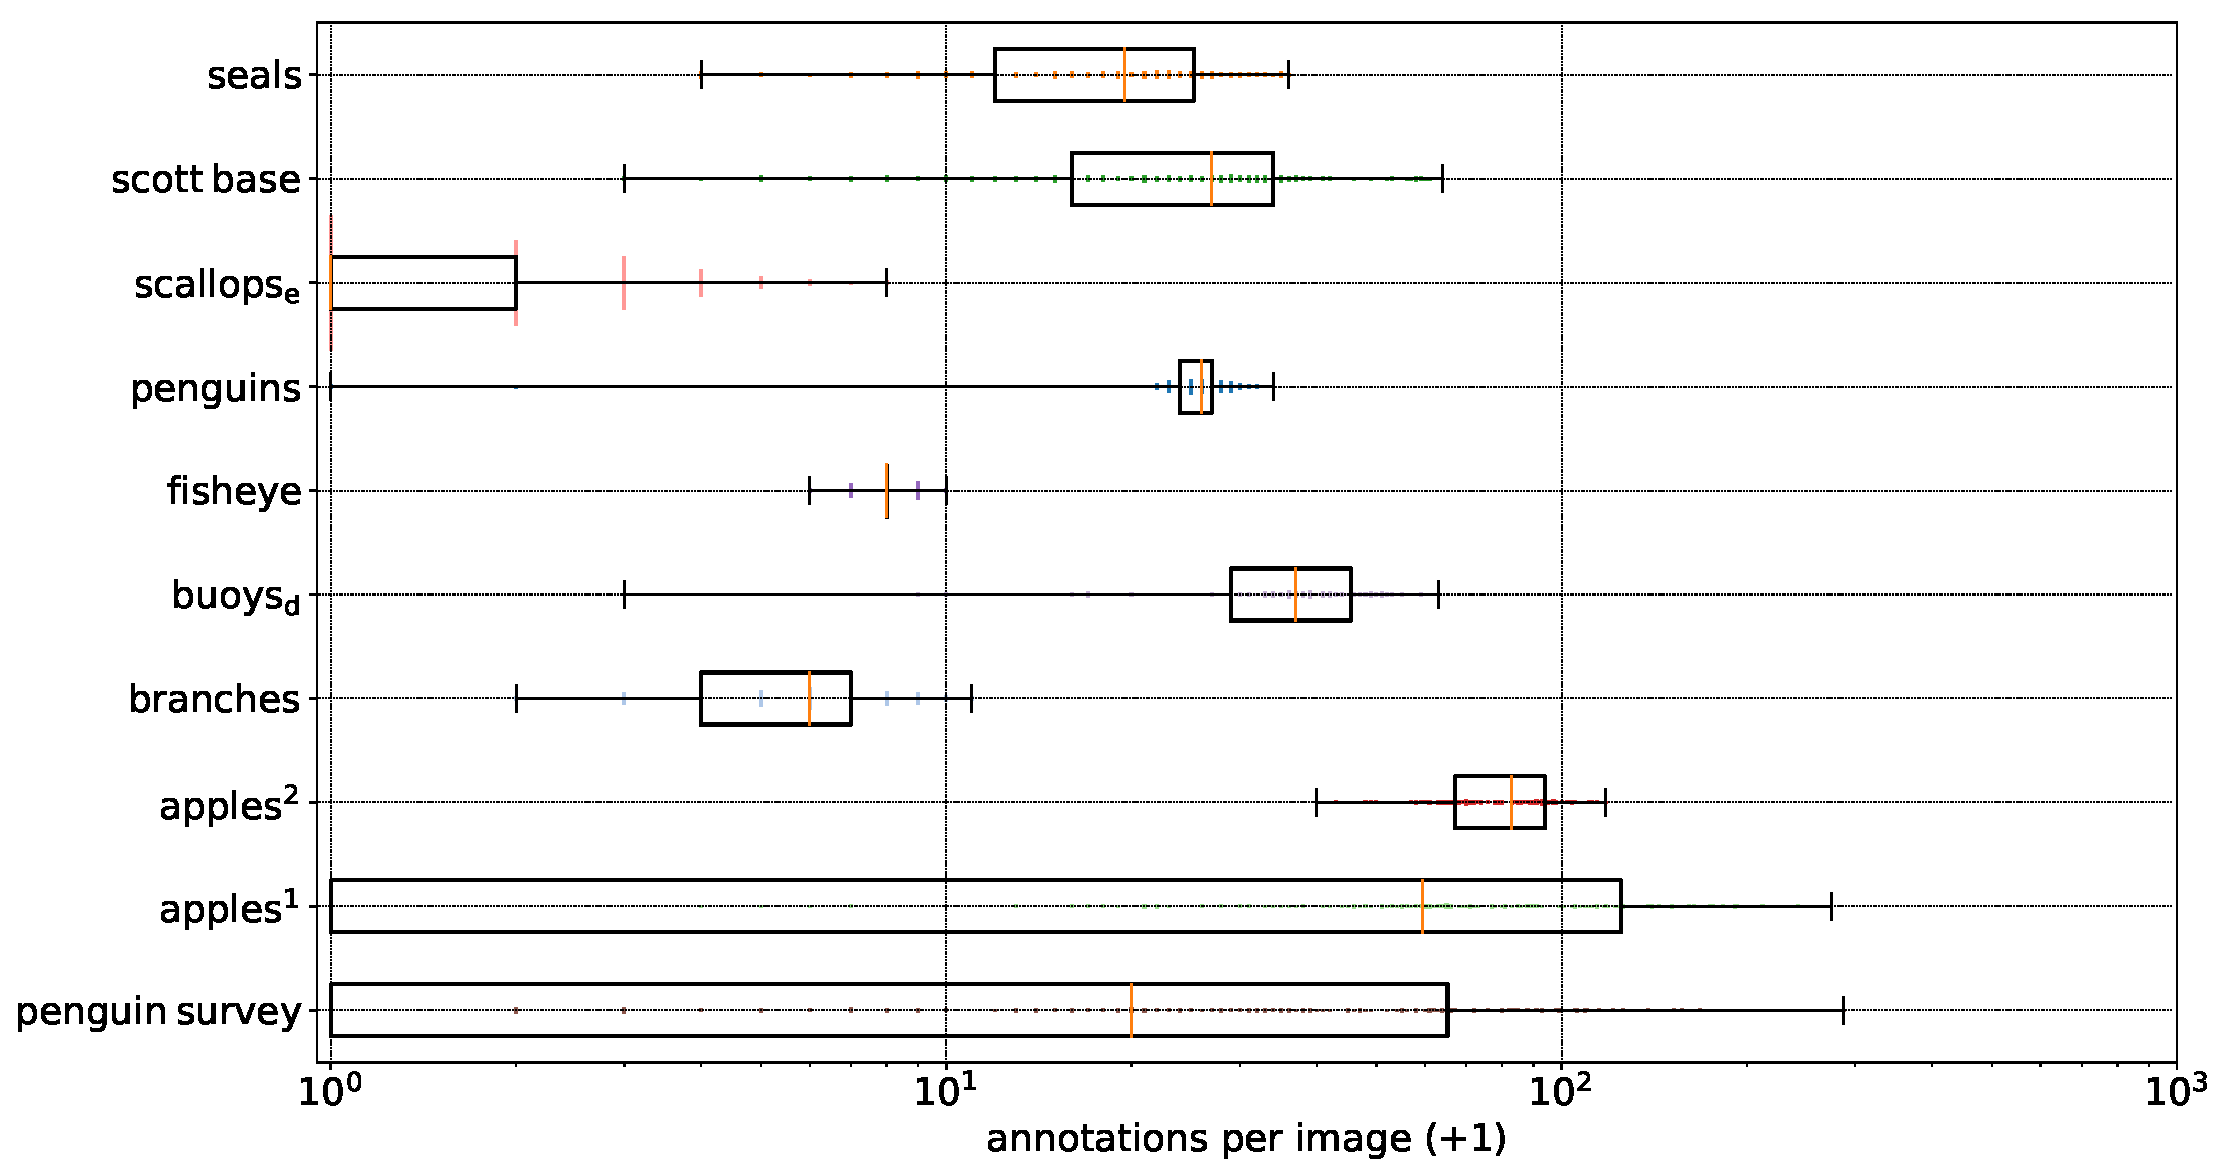
\includegraphics[width=1.0\linewidth]{charts/summaries/instances_boxplot.pdf}
\caption{ Distribution of object annotations per image, shown as a box plot with quartiles, range and median (red line) on a log scale. Vertical coloured lines show annotation counts for particular images. }
\label{fig:instances_image_plot}
\end{figure}

\begin{figure}[ht]
\centering
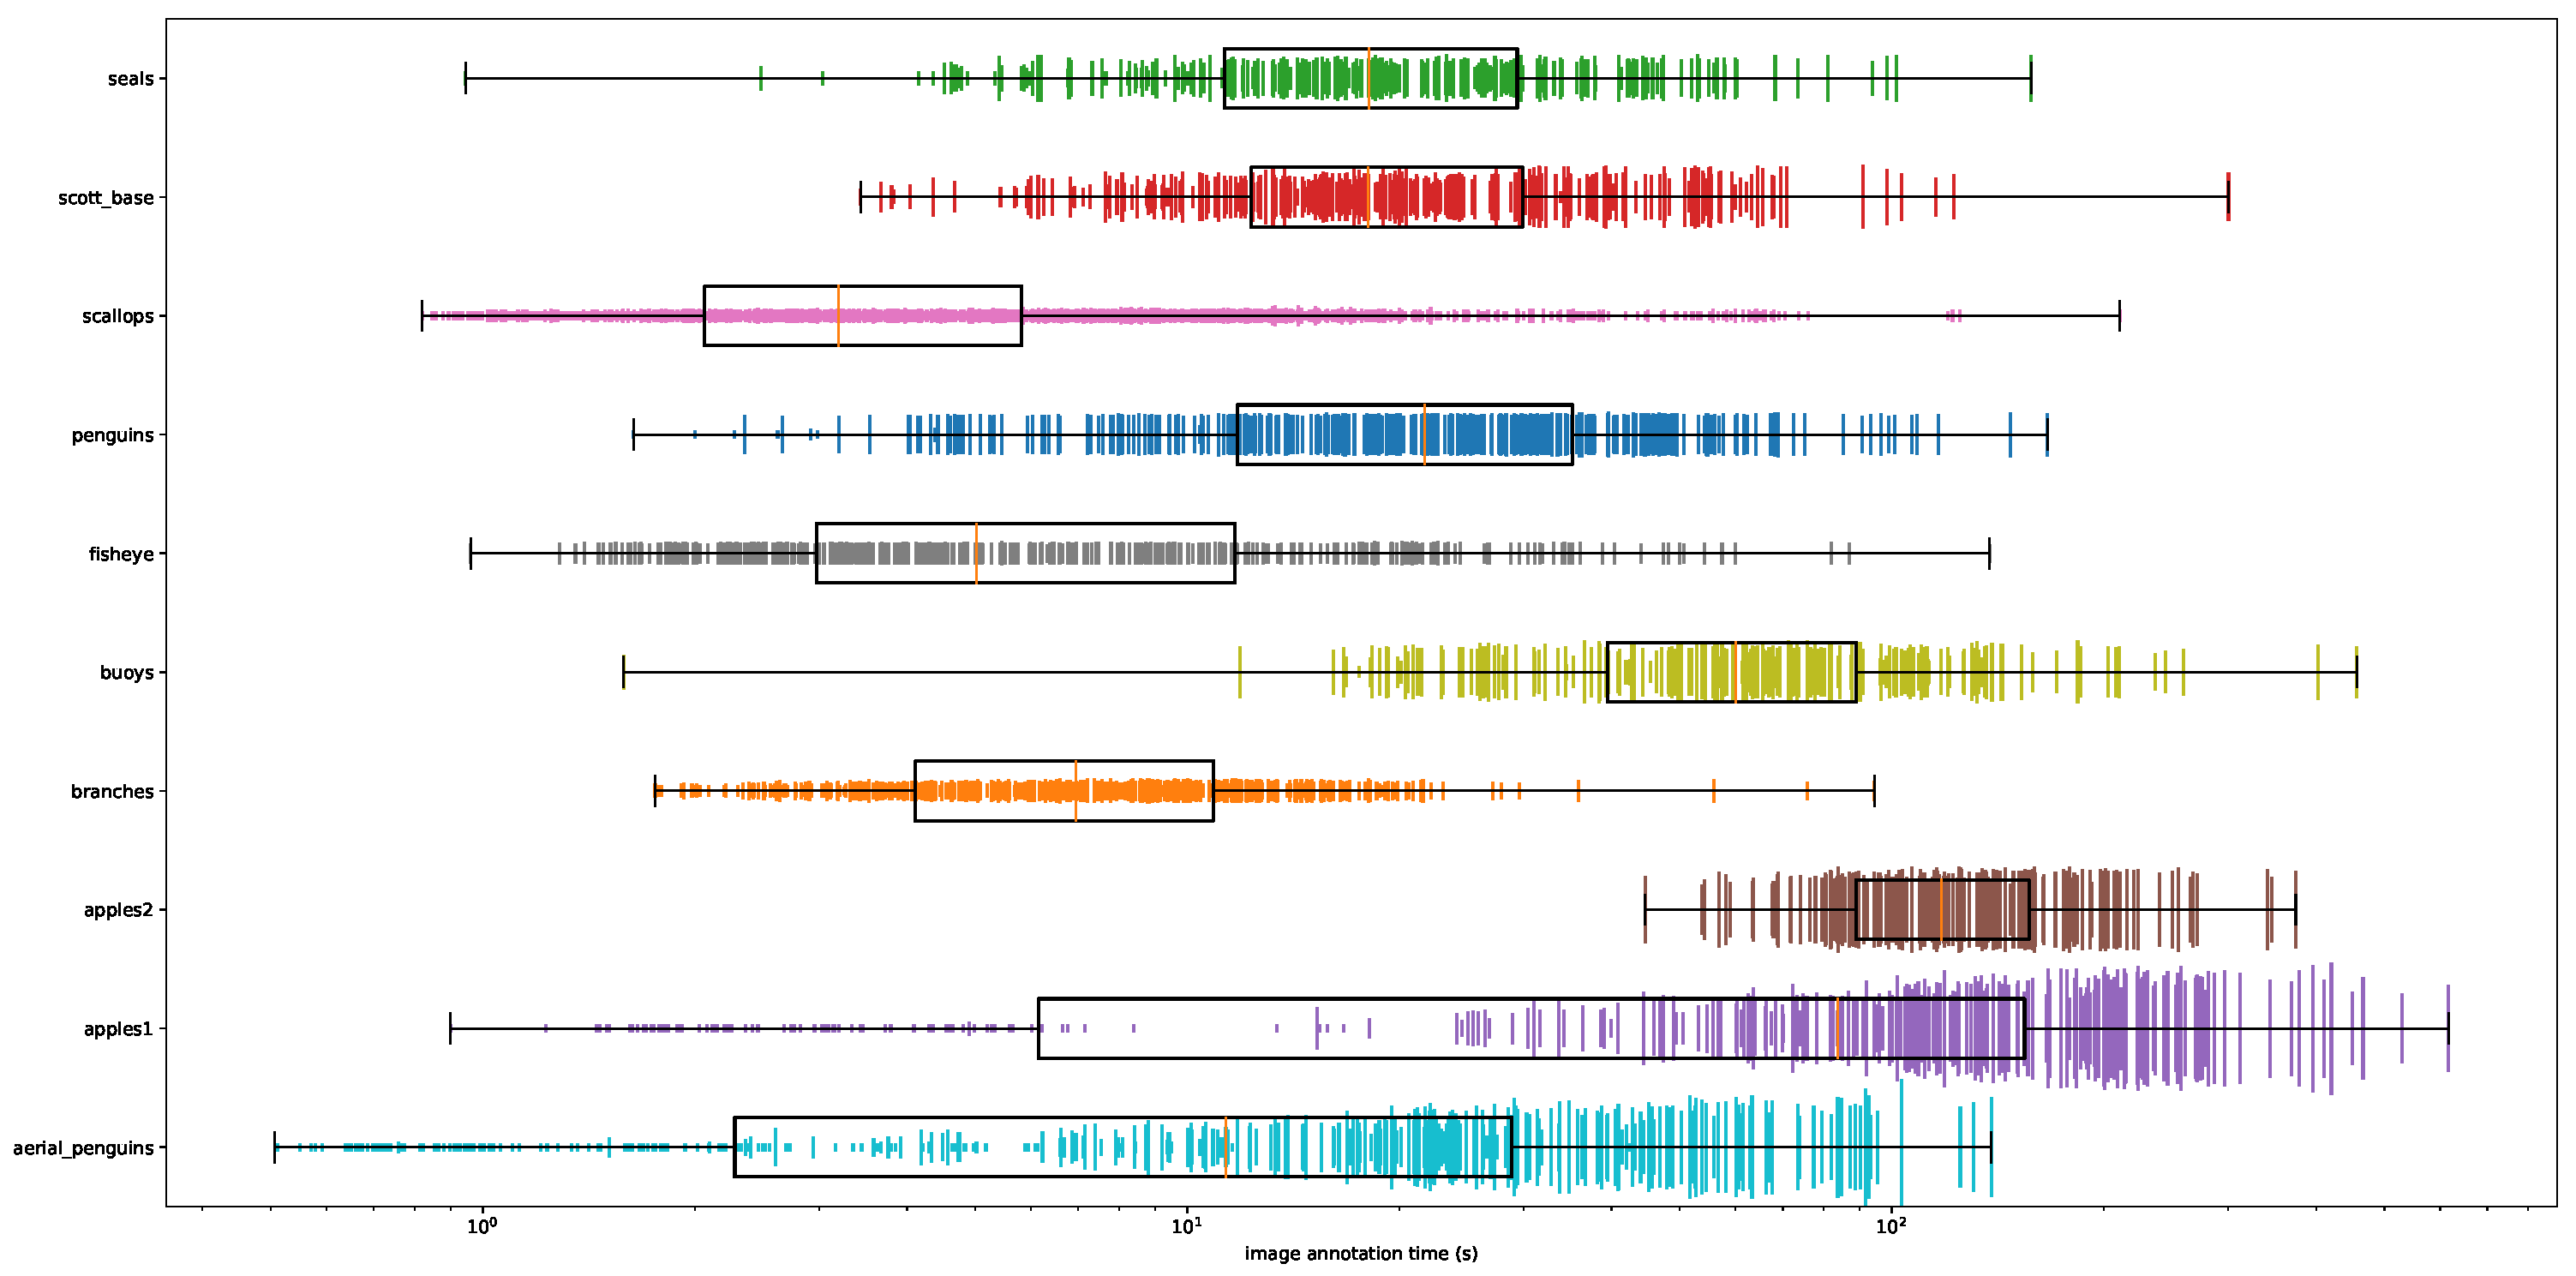
\includegraphics[width=1.0\linewidth]{charts/summaries/duration_boxplot.pdf}
\caption{ Per image annotation time distributions as box plot showing range, quartiles and median (red line). Vertical lines are individual images with line length proportional to to $\sqrt{|annotations|}$. }
\label{fig:duration_boxplot}
\end{figure}

The datasets in question have a wide range of instance distributions, shown in figure~\ref{fig:instances_image_plot}. Some such as \emph{apples2}, \emph{branches}, \emph{fisheye} and \emph{penguins} contain relatively uniform numbers of annotations. Others, especially \emph {penguin surveys}, \emph{scott base} and \emph{apples1}, contain a wide range (a few with several hundred annotations per image). One dataset, \emph{scallops}, contains very few annotations ($0.54$ per image), where most images are negative images.


\section {Annotation overview}
\label{sec:annotation_overview}

In this section, I try to break down any major trends seen from both annotation logs and the set of initial detections and final annotations. To begin with, I summarise the user actions and how they relate to the types of corrected detection. I also look at the object detection performance in validation, compared to the rate of true and weak positives for each dataset.

\subsection {Actions and corrections}

\begin{figure}[ht!] 
\centering
\begin{subfigure}{0.48\linewidth}
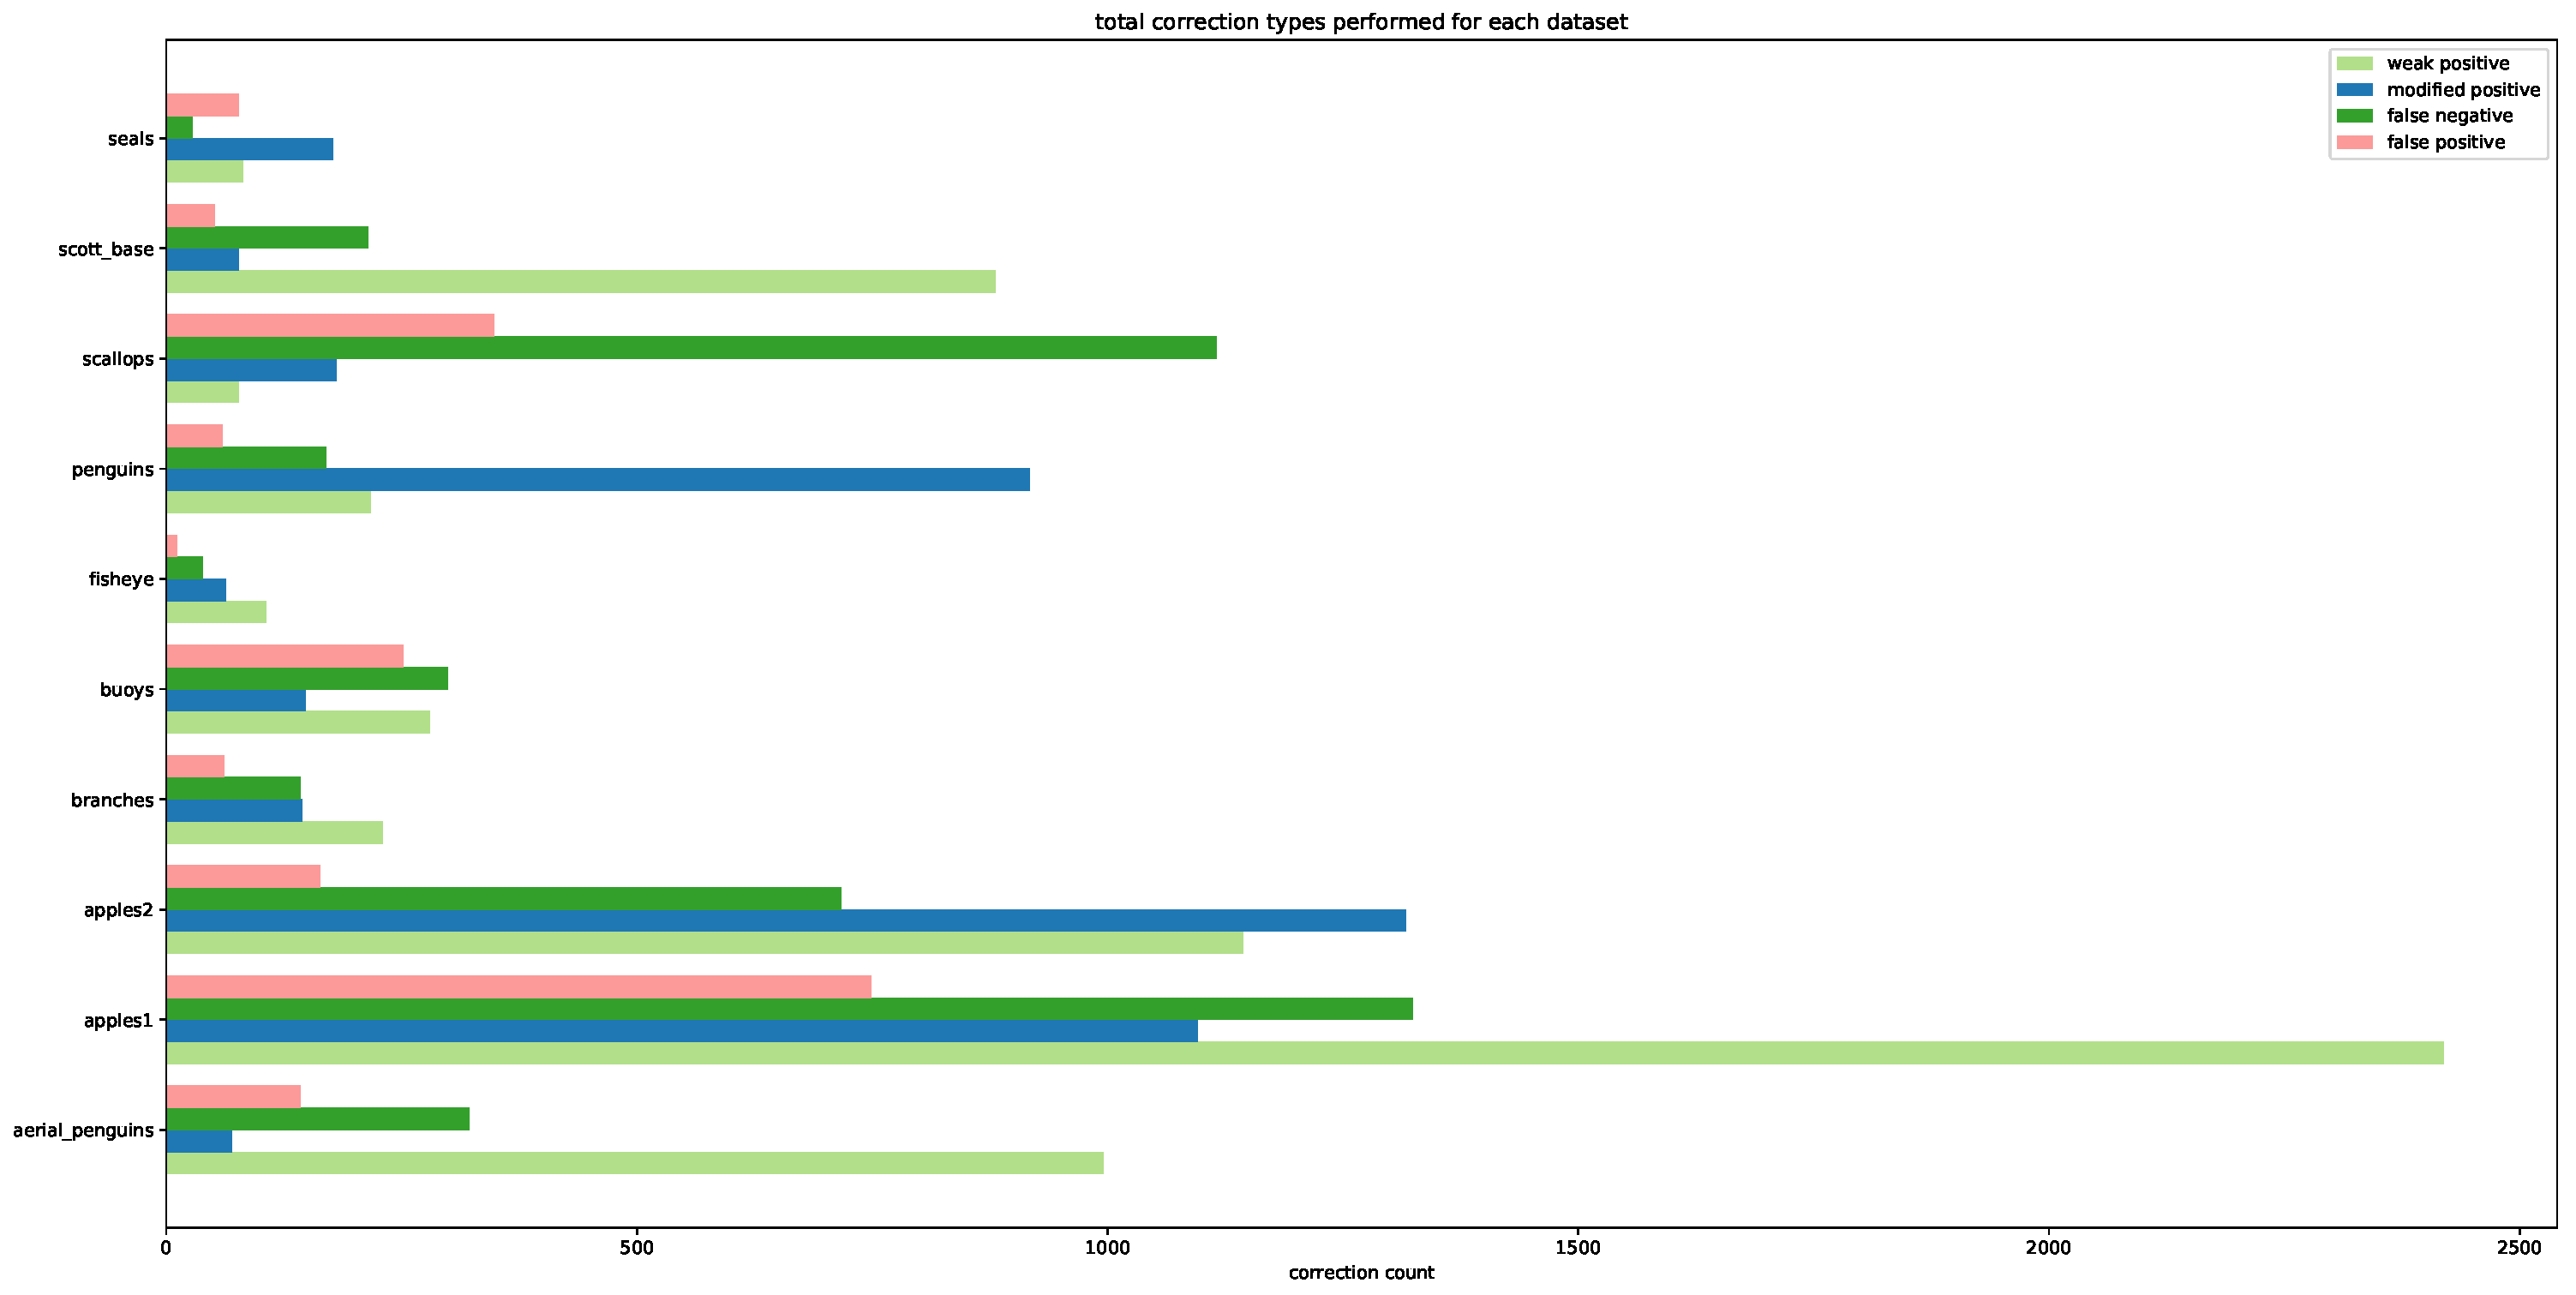
\includegraphics[width=1.0\linewidth]{charts/summaries/correction_counts.pdf}
\caption{}
\label{fig:actions_dataset_a}
\end{subfigure}%
\begin{subfigure}{0.48\linewidth}
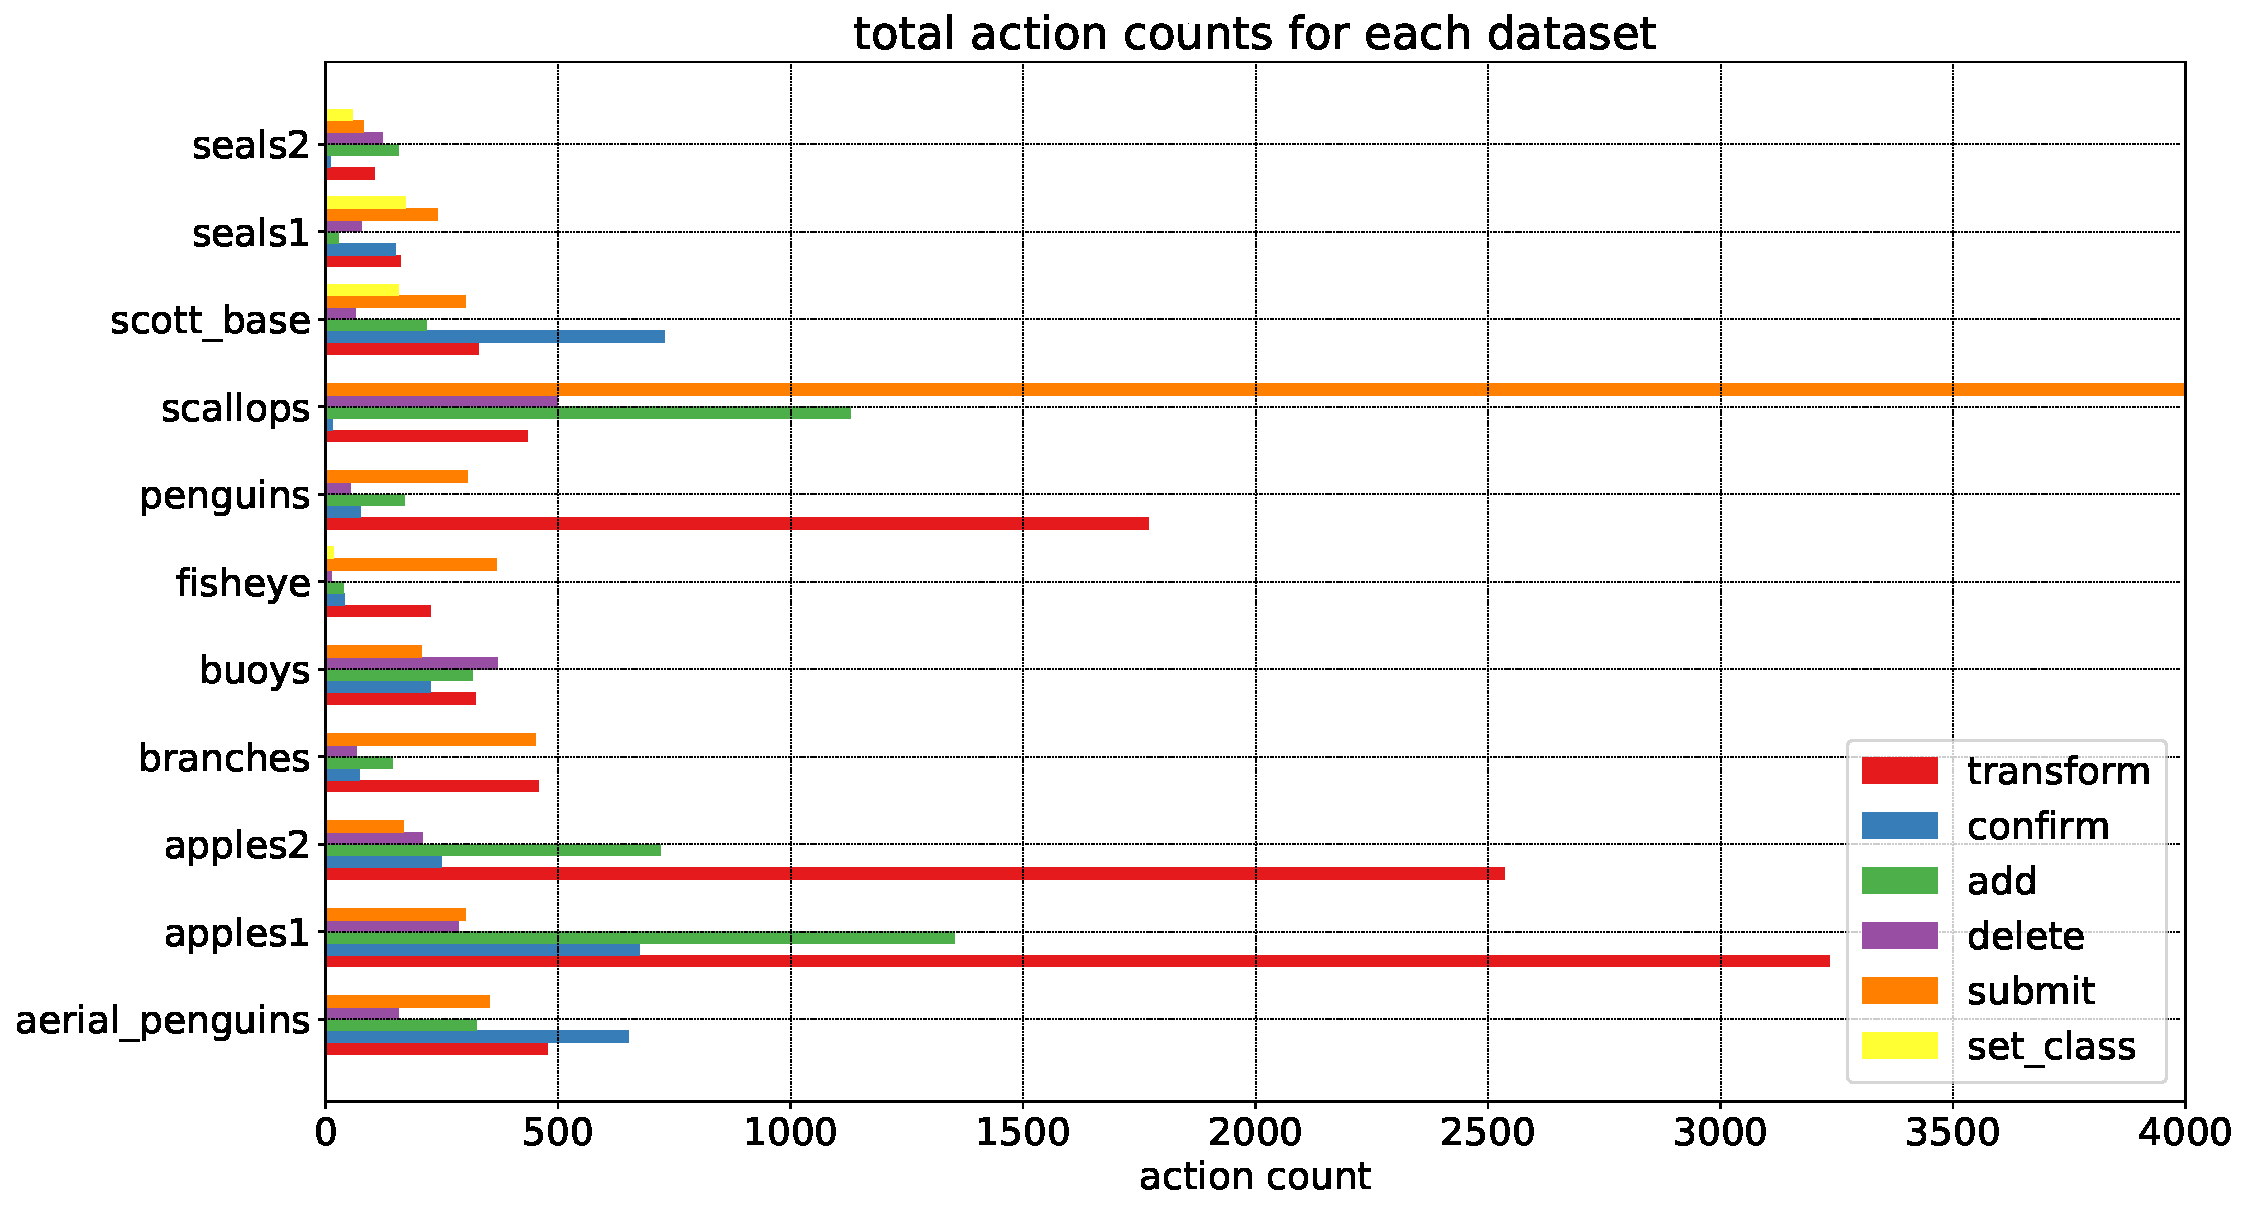
\includegraphics[width=1.0\linewidth]{charts/summaries/action_counts.pdf}
\caption{}
\label{fig:actions_dataset_b}
\end{subfigure}

\caption {(a) Total corrected detection types as a proportion of total annotation count. Note, totals do not sum to $1.0$ for two reasons: firstly false positives are shown, secondly positive detections are not. (b) Proportions of total actions. }
\label{fig:actions_dataset}
\end{figure}

\begin{table}[h!]
\caption{Validation accuracy at relaxed and strict IoU thresholds compared with proportions of corrected detections for each dataset}
\label{tab:validation_corrections}
\begin{adjustbox}{max width=\textwidth}
\begin{tabular}{llllllll}
dataset           & \shortstack{validation \\ $AP_{50}$} & \shortstack{validation  \\ $AP_{75}$} & positive & \shortstack{modified\\ positive} & \shortstack{weak\\ positive} & \shortstack{false \\ negative} & \shortstack{false \\ positive} \\
\toprule
$penguins$        & 99.4      & 90.5      & 82.6\%   & 12.3\%            & 2.9\%         & 2.3\%          & 0.8\%          \\
$branches$        & 95.7      & 69.6      & 76.8\%   & 6.4\%             & 10.2\%        & 6.3\%          & 2.7\%          \\
$seals$           & 95.5      & 93.1      & 93.4\%   & 4.1\%             & 1.9\%         & 0.6\%          & 1.8\%          \\
$seals_b$         & 92.0      & 81.5      & 87.3\%   & 1.1\%             & 0.0\%         & 11.7\%         & 8.7\%          \\
$scott\:base$     & 97.5      & 92.7      & 84.8\%   & 1.0\%             & 11.4\%        & 2.8\%          & 0.7\%          \\
$apples^1$        & 67.6      & 59.9      & 75.1\%   & 5.1\%             & 11.2\%        & 6.1\%          & 3.5\%          \\
$apples^2$        & 94.5      & 83.7      & 76.1\%   & 9.8\%             & 8.5\%         & 5.3\%          & 1.2\%          \\
$scallops_e$      & 92.8      & 78.4      & 62.3\%   & 4.9\%             & 2.1\%         & 30.4\%         & 9.5\%          \\
$fisheye$         & 99.3      & 90.7      & 91.8\%   & 2.4\%             & 4.1\%         & 1.5\%          & 0.4\%          \\
$buoys_d$         & 96.8      & 83.2      & 89.9\%   & 2.0\%             & 3.9\%         & 4.1\%          & 3.5\%          \\
\shortstack {$penguin$ \\ $survey$} & 90.9      & 73.3      & 89.5\%   & 0.5\%             & 7.5\%         & 2.4\%          & 1.1\%        \\ 
\bottomrule
\end{tabular}
\end{adjustbox}
\end{table}

The type of user actions performed, and the type of corrected detection can be seen in figure~\ref{fig:actions_dataset} and in more detail in table~\ref{tab:validation_corrections}. The two actions and correction types are different because: (a) multiple actions may be needed to correct one detection, and (b) one action can modify multiple detections, for example, deleting a group of false postives (this can be seen in the discrepancy in $apples^1$ where groups of false positives occur, to begin with, in images showing people, cars and wider angle shots). 

The action \emph{transform} is the most common action, by a long way, in the three datasets, and is significant in all other datasets (except \emph{scallop}, only because \emph{submit} outweighs the rest by such a large amount). This idea is not quite so well shown in the breakdown by corrected detection type, where \emph{modified positive} does not feature as prominently, mainly because the \emph{weak positive} category also includes low confidence detections which were transformed. This is not reflected in figure~\ref{fig:actions_dataset_b} because the user action \emph{confirm} is conflated with \emph{transform}. In cases where a user transforms a weak detection, it is confirmed at the same time yet counted as \emph{transform} only.

The most common action in three (and almost four) datasets is \emph{submit}, but this occurs for different reasons. In the \emph{scallop} images, it occurs because of the sparsity of object instances. In the \emph{fisheye} images, which have a very uniform visual appearance, the object detector reaches near human-level detection performance and there is nothing for the annotator to do except submit the provided detections.

One outlier which can be seen is $apples^1$, where the validation scores are much lower than $apples^2$, yet the correction statistics are very similar, with a similar positive proportion, albeit with $apples^1$ having higher proportions of false positive and false negative. It is not apparent exactly why this is the case, one possibility is that the validation set split is simply full of harder examples, and hence further investigation is necessary.

\subsection{Annotation rate}
\label{sec:annotation_rate}

\begin{figure}[ht!]
\centering
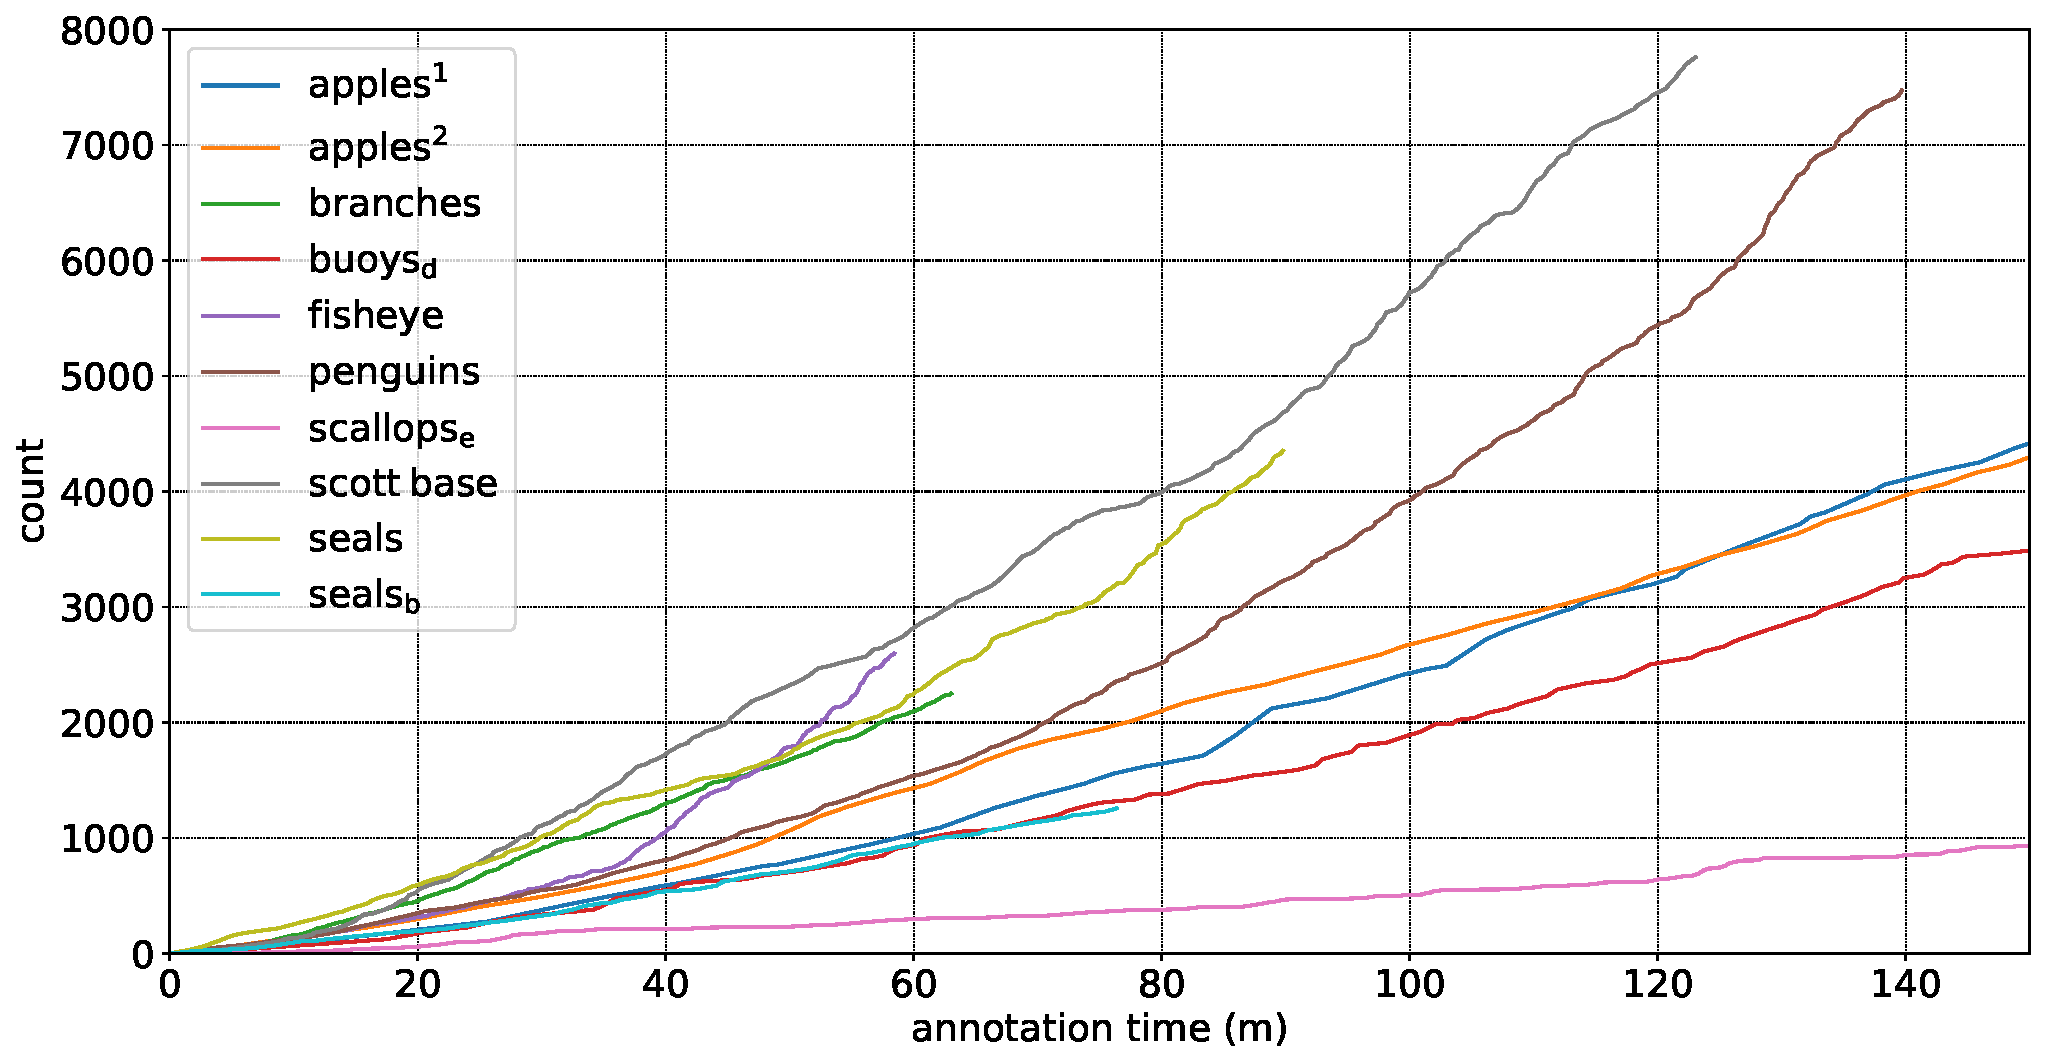
\includegraphics[width=1.0\linewidth]{charts/summaries/cumulative_instances_crop.pdf}
\caption{ Cumulative instances annotated (truncated to first 140 minutes)  }
\label{fig:cumulative_instances}
\end{figure}

\begin{figure}[ht!]
\centering
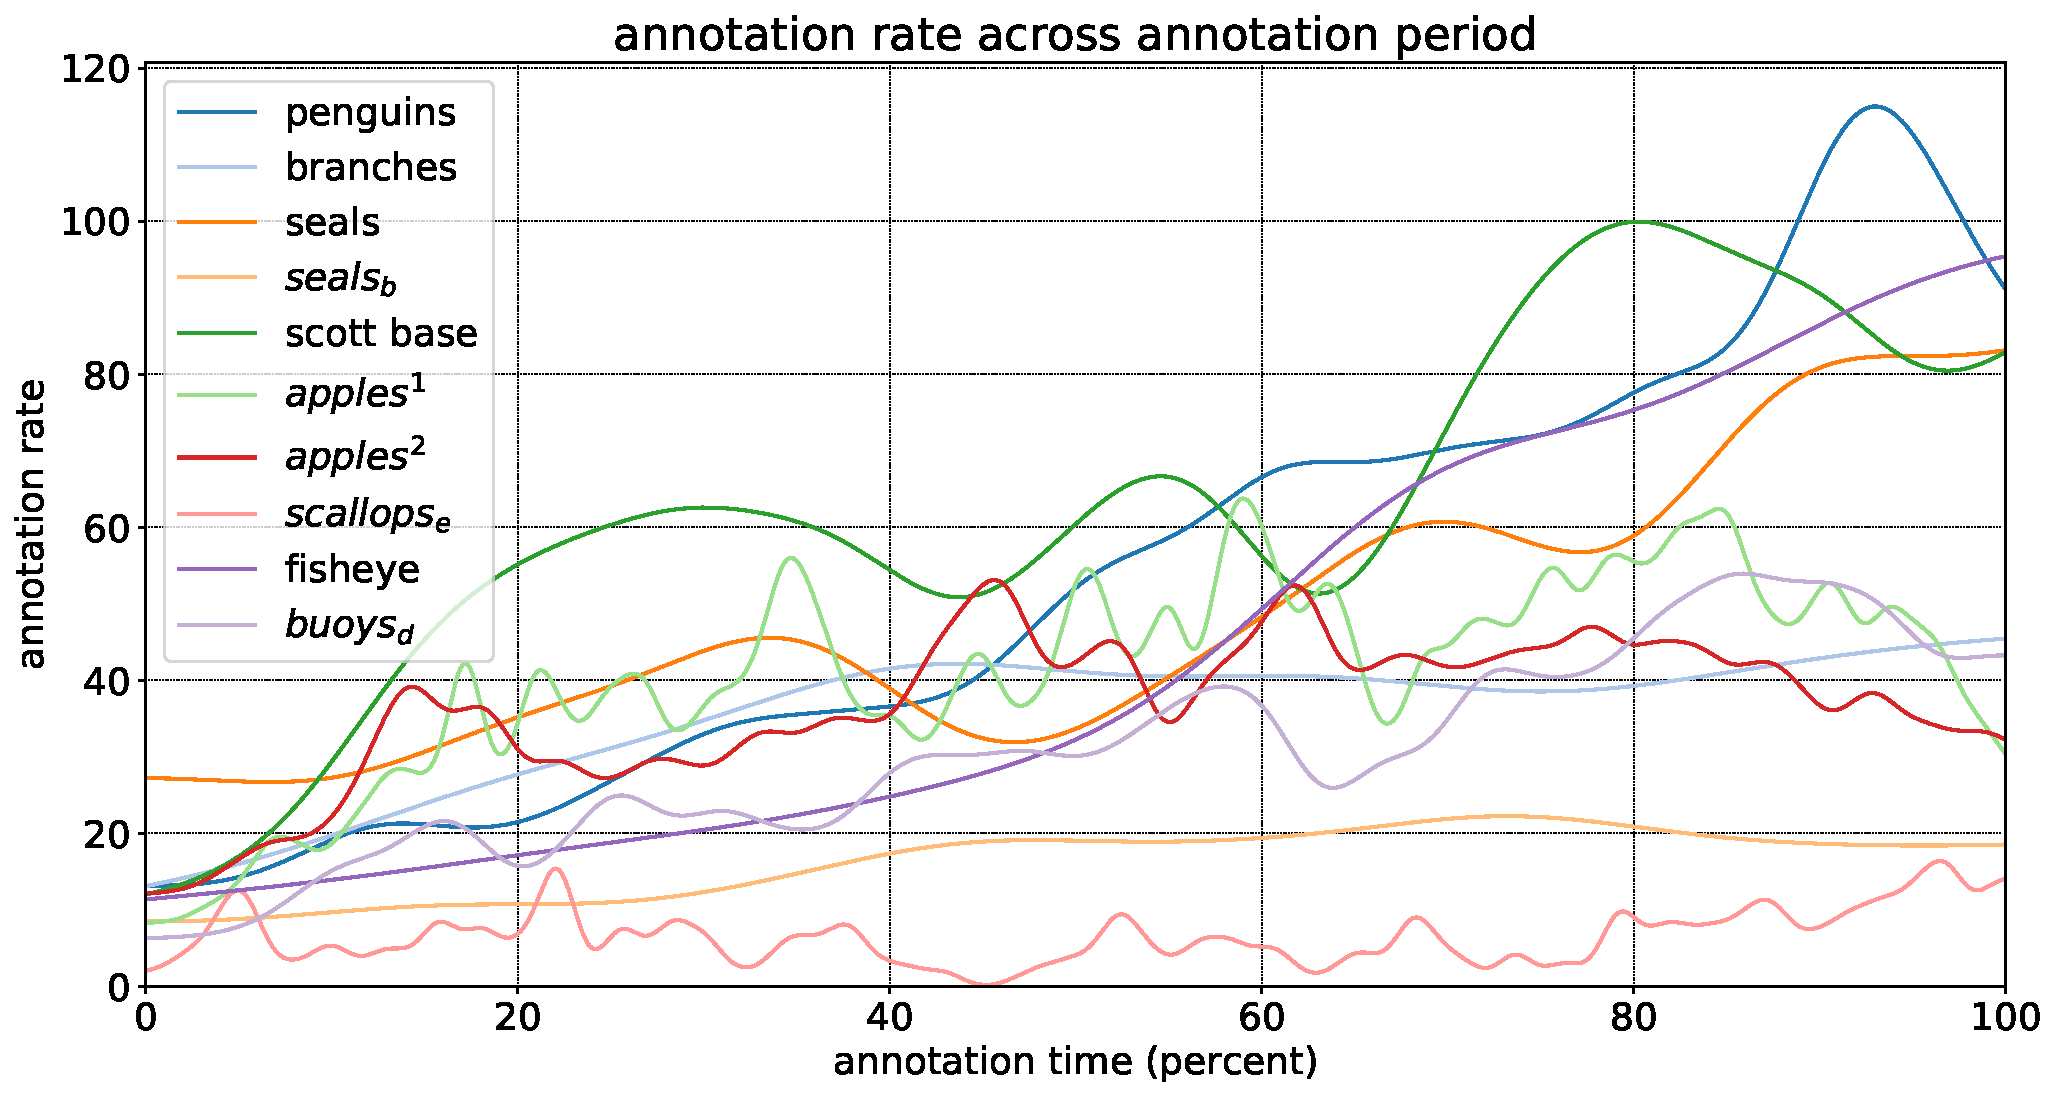
\includegraphics[width=1.0\linewidth]{charts/summaries/instance_rates.pdf}
\caption{ Annotation rate for all datasets (instances per minute) across annotation period, density plot with $\sigma=5minutes$ }
\label{fig:annotation_rate}
\end{figure}


\begin{figure}[ht!]
\centering
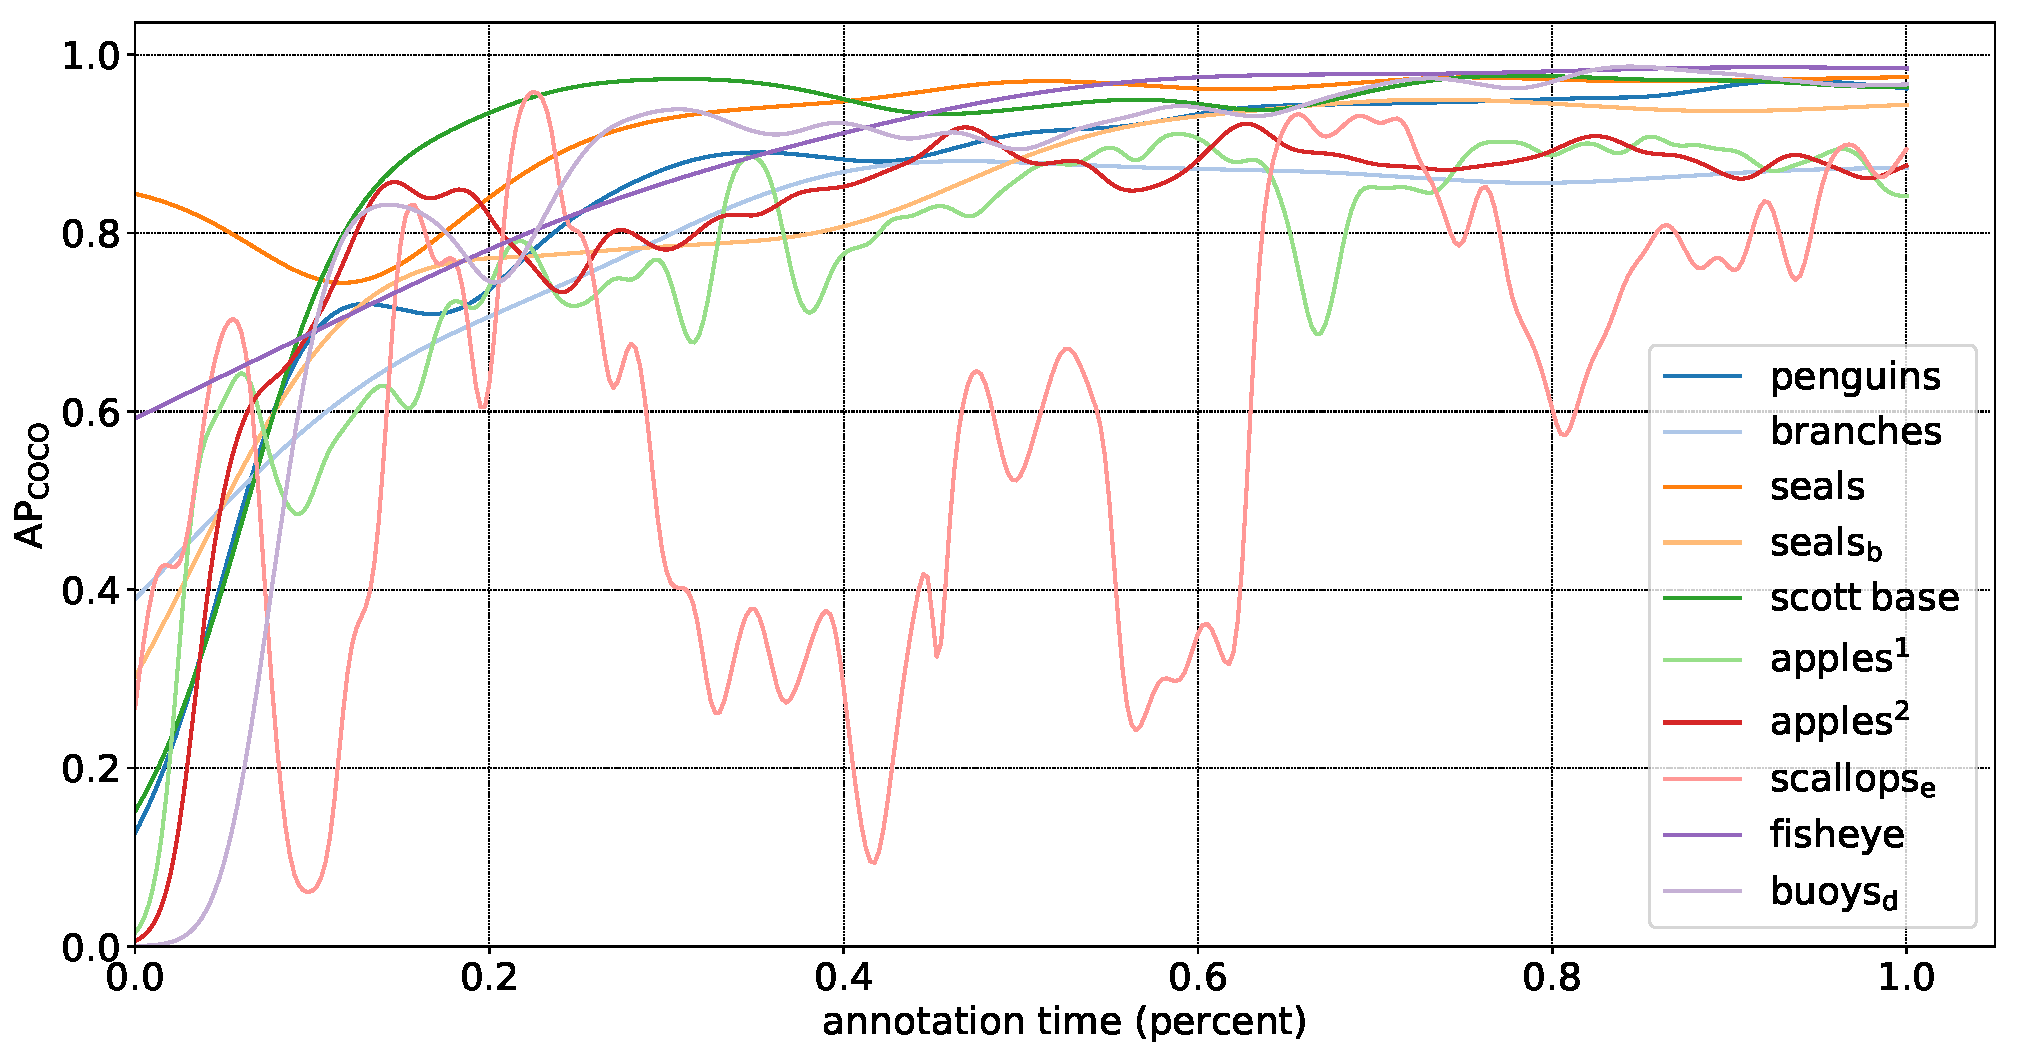
\includegraphics[width=1.0\linewidth]{charts/running_maps/overall.pdf}
\caption{ Locally weighted $AP_{COCO}$ of detections with respect to corrected annotations, providing a single metric taking into account all user corrections }
\label{fig:average_precision_test}
\end{figure}

The annotation progress can be most simply seen by examining firstly, the cumulative instances annotated in the given annotation time, and secondly, the rate of annotation occurring. Figure~\ref{fig:cumulative_instances} shows the cumulative instances over a $150$ minute period from the start of annotation. Figure~\ref{fig:annotation_rate} shows the rate of annotation (using a density plot of annotations added with a gaussian kernel of $\sigma = 5 minutes$). In this case the full annotation period is shown, where time is expressed as a percentage of total annotation time, instead of minutes.

A general acceleration in annotation can be seen in the  cumulative instances and more clearly seen in the annotation rate, although progress is far from linear. Time and instances are clearly not the only factors influencing annotation rate. 

The datasets with the most uniformity can be seen to provide the most benefit. They are the time series datasets, especially from video, where \emph{fisheye}, \emph{penguins}, \emph{seals}, and \emph{scott base} show the most clear benefit. These same datasets can be seen to be the ones which provide the most accurate detections, and also are the ones which achieve the highest validation accuracy (see table~\ref{tab:validation_corrections}).

Notably, missing from these figures is the \emph{penguin survey} dataset, as it is actually a combination of three annotation runs on separate parts of the \emph{penguin survey} dataset from different geographical locations. Discussion around this is given in section~\ref{sec:case_penguins}.

The scallop dataset is a particular outlier, the image selection policy changed from selection by maximum detection to sequential frame-by-frame at the first $25\%$ or $120 minutes$. Due to the sparseness of positive examples at various parts of the video sequences. The object detection accuracy can be seen to degrade at that same point figure~\ref{fig:average_precision_test}, possibly because of the influx of negative examples or a domain shift (the images varied in view angle between runs, and the light on the \gls{ROV} became intermittent). Towards the end of annotation, the object detection performance recovers, along with the annotation rate. Given this result, it would seem prudent to focus image selection policy on obtaining a balanced training set. 

\section{Verification threshold}
\label{sec:verification_threshold}

Behind any tool based on verification (be it cross verifying human annotation, or verifying machine predictions), there are implicit thresholds which are deemed acceptable and are going to vary between person to person and even within one person's verification effort. 

How often an object detector can exceed the annotator's verification threshold, will largely determine the level of assistance provided by a verification based tool (along with other factors like false positives and accurate classification). For the datasets annotated here, this can be seen in table~\ref{tab:validation_corrections}, where there is a range between $60\%$ and $90\%$ of verified detections accepted as is (across the whole annotation effort). 

\subsection{Algorithmic limits}
\label{sec:machine_limits}

The benefits of a \gls{VBA} tool are limited by the object detector. The benefit provided can (and does) increase as more images are annotated and the object detector becomes more accurate, but is also bound by the algorithms used by the object detector. Some datasets annotated here, were negatively impacted by the inability of an anchor-box based object detector to detect overlapping objects, particularly in the two apple datasets and \emph{scott base}. 

No matter how much training data is provided, a user will always be required to correct problems caused by artefacts of the object detector; in the case of apples, this means adding in missed detections occurring in a large bunch of apples, and addressing ghost detections which occur between detections at times. During the annotation of both apple datasets, it seemed like a large number of the corrections required were addressing artefacts of the object detector.

As object detectors improve over time this will become less of an issue. Object detectors may arise which can more naturally distinguish multiple near overlapping objects, or 3D object detectors may be able to separate the overlap by depth. An alternative solution may be to use annotations with more specific localisations, such as pose recognition. A more specific localisation can help with separating objects which overlap, at a cost of larger annotation effort per object.


\subsection{Distortion on Average Precision}
\label{sec:distortion_precision}

\begin{figure}[ht]
\centering
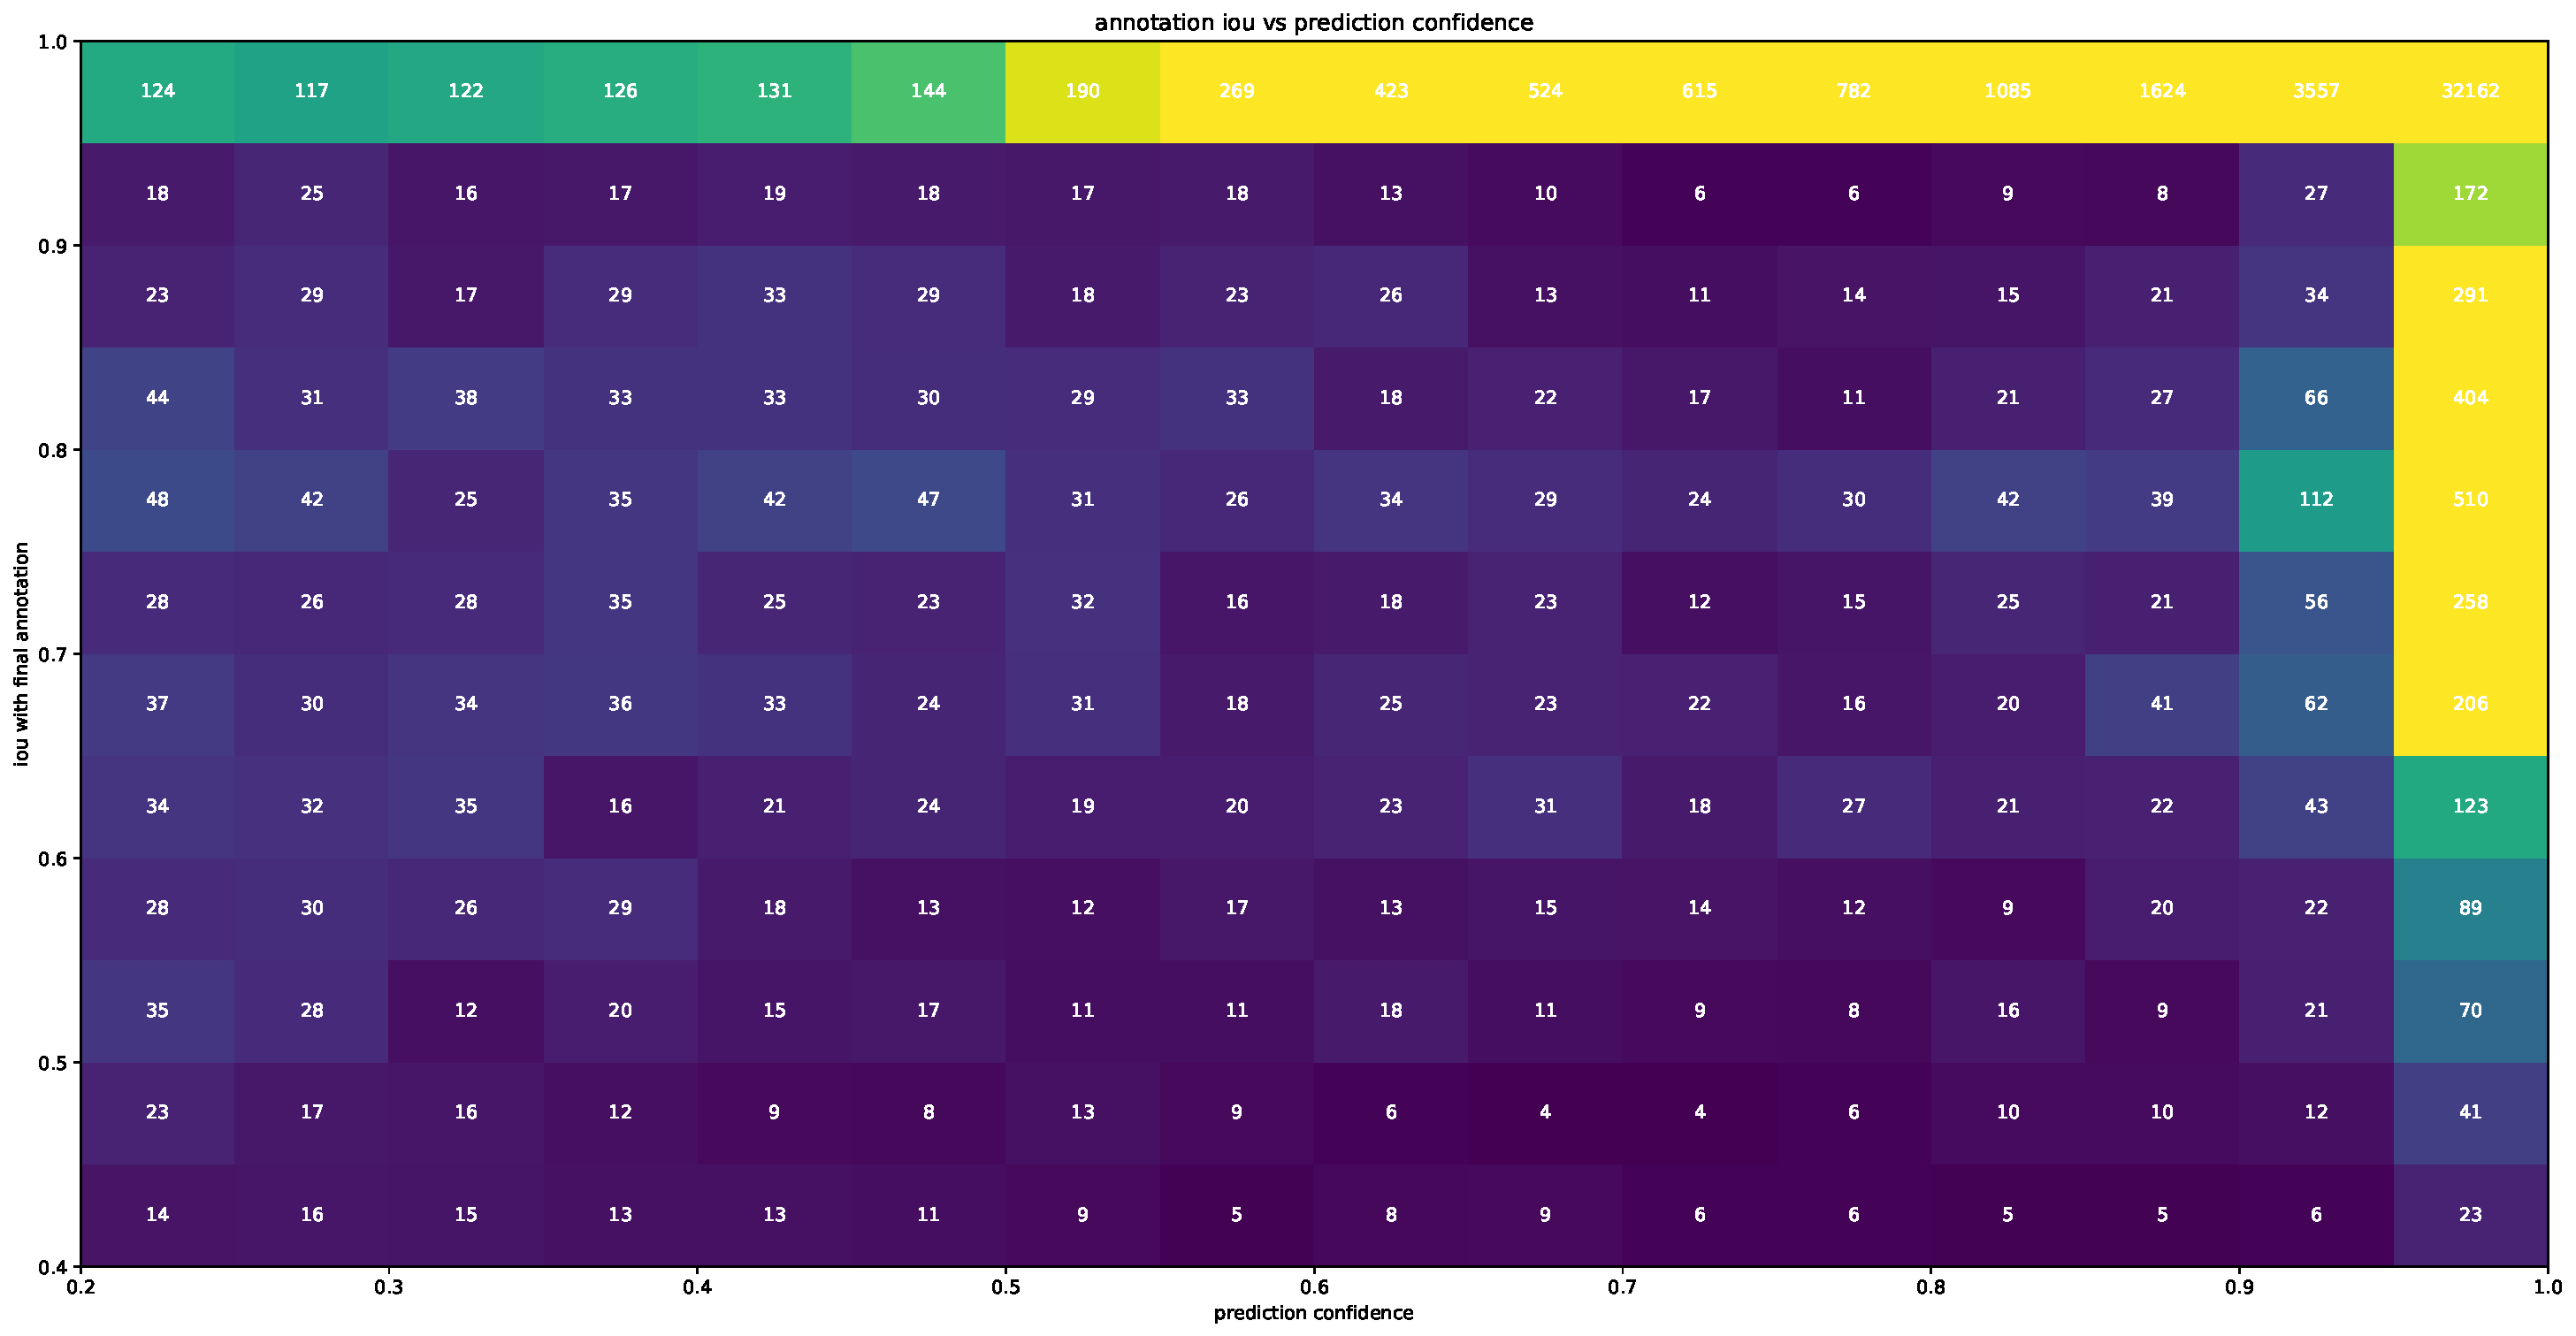
\includegraphics[width=1.0\linewidth]{charts/scatters/confidence_iou.pdf}
\caption{ IoU of detection with respect to final annotation vs. confidence, for detections (modified or otherwise) included as an annotation. Colours encode the same histogram counts as written in the text. }
\label{fig:iou_confidence}
\end{figure}

One aspect of note is that there exists a gap between the $AP_{COCO}$ reported in figure~\ref{fig:average_precision_test} and the $AP_{COCO}$ from testing the object detector against its validation set seen in table~\ref{tab:validation_corrections}. The validation set accuracy is much lower in all cases, and the reason for this is that the human annotator has a lower threshold for acceptance. This threshold can be seen in figure~\ref{fig:iou_confidence} where a majority of detections are accepted unmodified (and as such have \gls{IOU} overlap of $1.0$ with the final annotation for the purpose of \gls{AP} calculations).

The \gls{AP} metric has some systematic differences when used in this way, meaning it is not comparable with the validation set accuracy. If a detection is accepted \emph{as is} by the human annotator, it is considered in this metric to be $100\%$ precise (even at $0.95$ \gls{IOU} threshold), which is an unrealistic level of agreement. If a human was to draw a box, natural variability would make it much more likely to have some variation, and the predictions from the object detection model will also often not match with such precision.

It could be argued that the metric created from human corrections was the better one, simply because it does include that level of tolerance. Where the scoring calculated from testing on the validation set may penalise tiny differences, arising from natural variation, the score based on human corrections, takes into account the desired level of localisation precision and small differences, that arise because of uncertainty or irrelevant details are ignored.

\subsection {Measure of localisation precision}
\label{sec:localisation_precision}

Figure~\ref{fig:density_iou} shows in more detail the distribution of \gls{IOU} overlap for detections which have been modified. The density of transformed detections peaks at around $0.80$--$0.85$ depending on the dataset. It can be reasonably assumed that the real accuracy of the detections, which are used unmodified, would lie between that peak and $1.0$. Human annotation also has some degree of variability (reference \cite{Papadopoulos2017} gave a mean \gls{IOU} of 88 overlap for a box input method with Pascal VOC ground truth).

One minus the peak density seems like a reasonable surrogate measure for the human verification threshold. From the datasets annotated in this thesis the \emph{penguins} dataset annotation has the lowest threshold, at approximately $0.15$, and as a result it seems likely the most precise localisation. For the \emph{penguin survey} the threshold is highest at around $0.35$. This makes sense, because counting was emphasised as opposed to precise annotation, so it is natural that the localisation threshold is higher. 


\begin{figure}[ht]
\centering
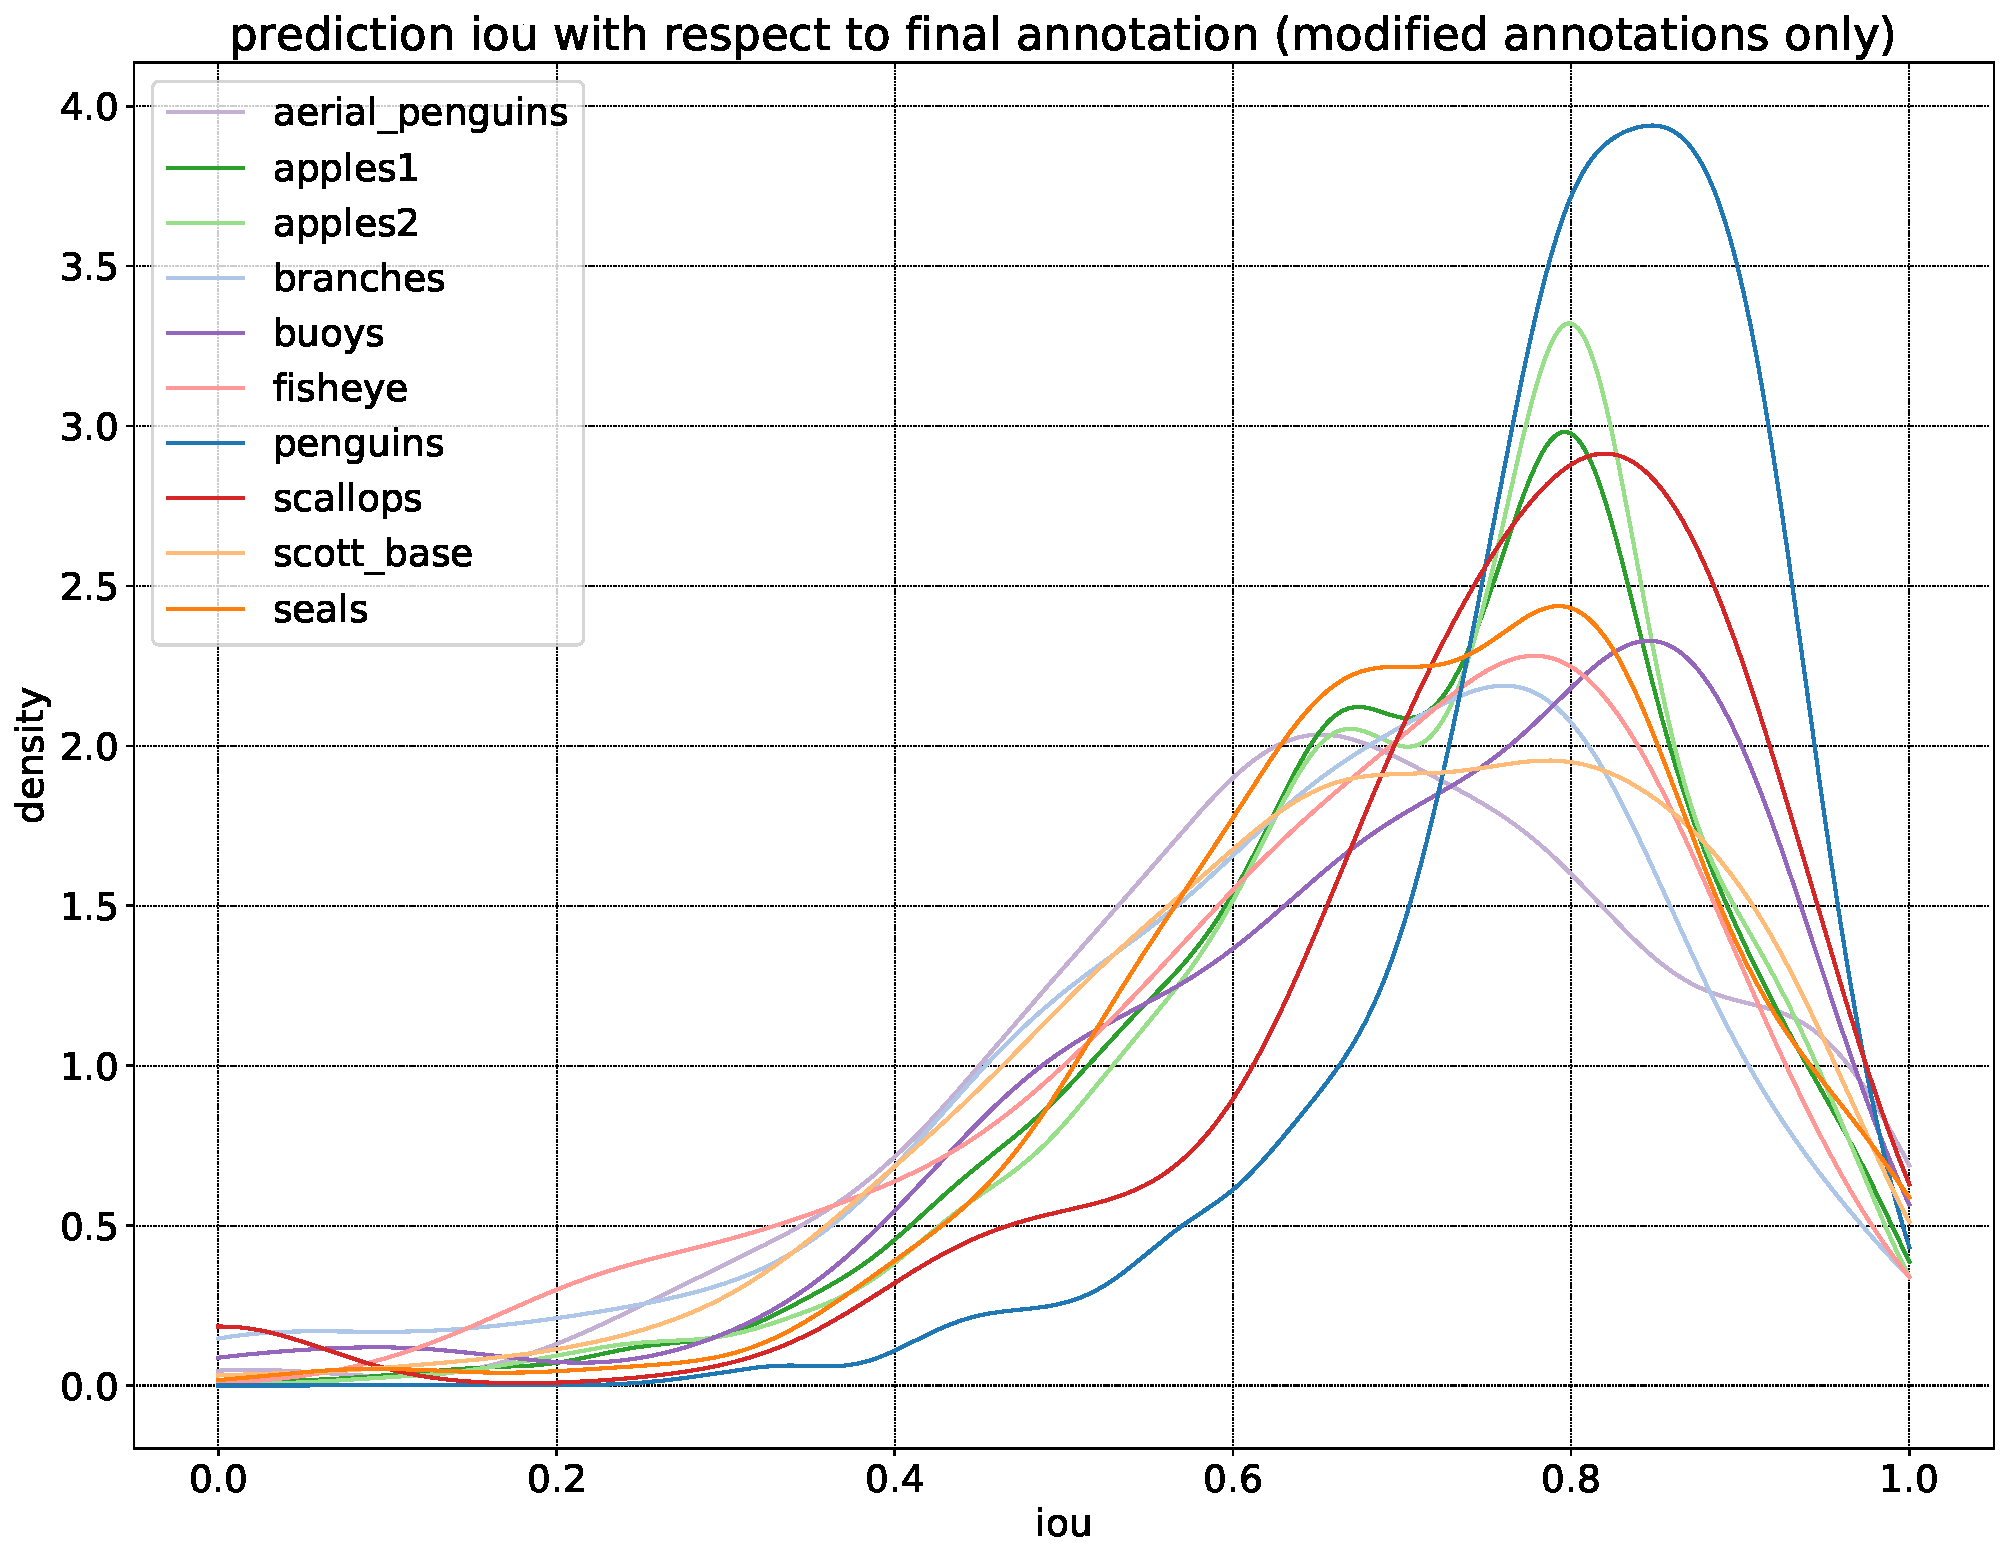
\includegraphics[width=1.0\linewidth]{charts/scatters/iou_dataset.pdf}
\caption{ Density plot of IoU overlap for detection with respect to annotation, for transformed detections. }
\label{fig:density_iou}
\end{figure}


\section{Localisation vs. confidence}
\label{sec:localisation_confidence}

One of the premises of providing the ability to pick and choose low confidence detections (using the two threshold method), is that weakly detected objects are often being localised well. Figure~\ref{fig:iou_confidence} shows that is the case, as a significant proportion of final annotations had both low confidence and  precise localisation (as well as a proportion having high confidence and imprecise localisation).


\begin{table}[h]
\caption{Breakdown by dataset of detections included as an annotation; confident if $ p > 0.7 $, precise if $ IoU > 0.85 $ with respect to final annotation} 
    \centering
\noindent\resizebox{1.0\textwidth}{!}{%    
\begin{tabular}{l l l l l l l l || l}

& seals  & $\mathrm{seals_b}$ & $\mathrm{apples^1}$ & $\mathrm{apples^2}$ & penguins & fisheye & branches & total  \\
\toprule
high confidence, imprecise & 1.2\%  & 0.4\%     & 5.1\%      & 7.9\%      & 7.5\%    & 1.4\%   & 5.3\%    & 5.5\%  \\
low confidence, precise & 7.2\%  & 6.3\%     & 6.5\%      & 5.5\%      & 1.2\%    & 5.6\%   & 7.5\%    & 5.5\%  \\
high confidence, precise   & 90.2\% & 93.1\%    & 81.5\%     & 80.0\%     & 89.7\%   & 89.9\%  & 79.6\%   & 83.7\% \\
\bottomrule
\end{tabular}
}
\label{tab:confidence_precision}
\end{table}

In the implementation of object detection neural networks, such as the one used in this work (see chapter~\ref{chap:object_detection}), the sub-network for classification is separate from localisation, and localisation is predicted for all anchor boxes regardless of classification performance. It is not surprising therefore, that sometimes localisation is predicted well and yet the object is not classified well.


\section{Number of instances}
\label{sec:instances_discussion}

The instance distribution in each image has clear implications for verification based image annotation. Verifying several instances at once can be more efficient than one at a time, but verifying too many instances concurrently increases cognitive load (the very problem human-in-the-loop machine learning seeks to address). 

Despite the ability to zoom into a small part of an image, in order to submit an image, the user must review the whole image or remember which parts have been checked. For this reason, when images become excessively large, they should be split into pieces which can be easily verified without too much use of navigation.

This can be similar to a user interface for navigating search results, where showing several results at once is much faster for a user to peruse, than showing them one by one. However, if too many results are shown on each page, the results become lost in the crowd. A pair of studies found users do not look at results beyond 30 per page \cite{PunchoojitLumpapun2017, Zhou2007}.

The dual threshold approach helped in this regard, by highlighting areas of uncertainty. For some datasets, \emph{penguin surveys}, \emph{apples1} and \emph{apples2}, the number of instances made it hard to keep track of progress when verifying the whole image. Combined with uncertain instances, which are difficult to see without zooming, checking to ensure all annotations are present becomes difficult.

The dataset \emph{scott base} also suffers a little from this problem. The images are much wider than they are long, making navigation somewhat tedious, and verifying the whole image much harder by having to zoom right out to check the whole image. In future some method of marking parts of an image, as checked, may be useful.

\section{Algorithmic bias}
\label{sec:machine_bias}

Algorithmic bias can cause significant problems for tools based on verification in two ways: (a) it can change the human decision making process and (b) it can cause a feedback loop, where error introduced by the algorithm becomes magnified.

A human annotator may be influenced by an object detector's predictions. For instance, a yellow box around part of an image might suddenly appear much more likely to be an object than it would have otherwise seemed. A user may become reliant on features of the annotation interface, such as the ability to show weak detections. If a user only looks at the weak detections shown, it may significantly reduce the likelihood of finding missed detections which were not detected at all. Repeated inaccurate detections may fatigue an impatient annotator and have them lower their standards, leading to worse quality annotation. 

Subtle error may not even be noticed by a human annotator, for example,  if during implementation a bug was introduced where bounding box localisation was slightly incorrect. It was also noticed that training with more ``odd'' dimensions for training images could cause similar issues with inaccurate box estimation, because of changes in anchor box alignment with respect to the edge of the image, unequal up and down scaling and edge padding used on convolutions. Such errors may not be obviously noticeable and not corrected by a human annotator.
 
Any of the above influences may cause annotations to be less accurate. A much bigger problem is that if the inaccurate annotations have some kind of systematic bias, and then are fed back into training the object detector, a feedback loop can occur. A consequence is that predictions may ``wander'' over many iterations (dependent on image resolution). Subsequent predictions may move slightly, perhaps not in a noticeable way, but after a period of feedback, end up moving significantly. Because the annotations move over time there would be no way to correct the issue, because it would be necessary to correct all the existing annotations, many of which would have various degrees of this systematic bias. This issue can be seen to have affected the initial run of penguin counting (discussed in section~\ref{sec:case_penguins}).  

Such an algorithmic bias would have one of two impacts, it would either make annotation efficiency very low (and negate any useful properties of \gls{VBA}), or it would severely degrade object detection accuracy (studied in section~ \ref{sec:noise_sensitivity}), which would then in turn require more human effort, or worse accuracy again. It is therefore something to be very concerned about for an annotator, especially near the beginning, not to introduce any accidental bias, and for the author of a \gls{VBA} system where any kind of algorithmic bias, when iterated, may completely negate any useful assistance provided to an annotator.


\subsection{User engagement}
\label{sec:engagement}

One aspect not discussed previously is that of user engagement. It can turn image annotation, which is otherwise a very tedious task, into an engaging and interesting process. A few quotes from people who have used the system:

\begin{displayquote}
``It's actually really rewarding to watch the system actually learn as you go!''
\end{displayquote}

\begin{displayquote}
``I noticed that towards the end of the image set the software was accurately picking nearly every scallop around the same time as I positively identified them which is great.''
\end{displayquote}

\begin{displayquote}
 ``It is not a problem to keep going, as it is a bit addictive.''
\end{displayquote}

\begin{displayquote}
``I can definitely see that application being astoundingly useful! Certainly the fastest I've ever annotated a field of Chinstraps[penguin]!''
\end{displayquote}

The benefit, as a rapid prototyping tool, cannot be easily quantified, but the immediate feedback provided by the system seems to be a very useful tool in assessing model performance and qualifying areas of strength and weakness. The user may actively explore unlabelled images and check performance under a wide variety of conditions.


\section{Case study: counting Ad\'elie penguins from aerial photographs}
\label{sec:case_penguins}

\begin{figure}[pht!]
\centering
\begin{subfigure}[t]{1.0\linewidth}
  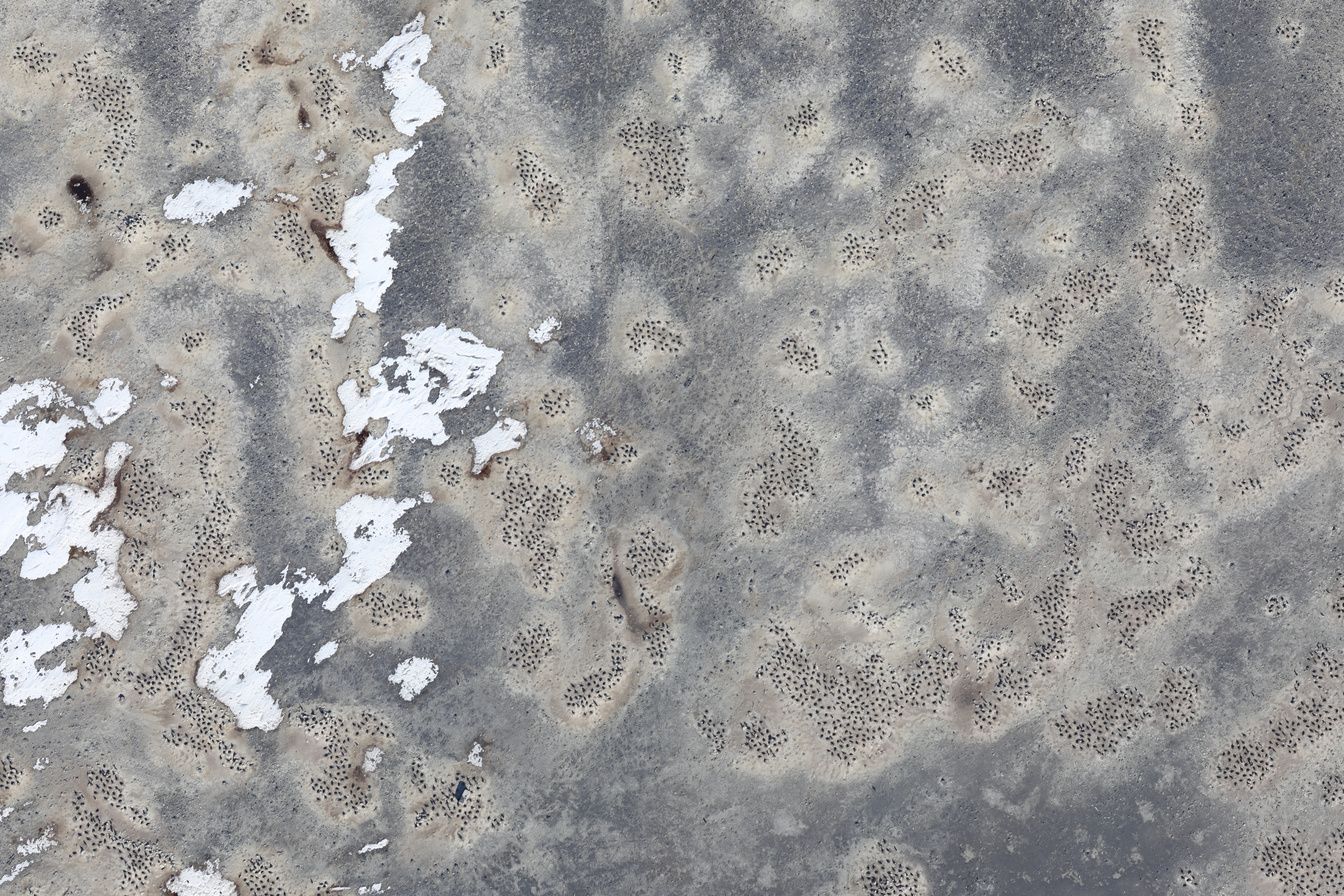
\includegraphics[width=0.475\linewidth]{figures/annotation/penguin/hallet_large.jpg}
  \hfill
  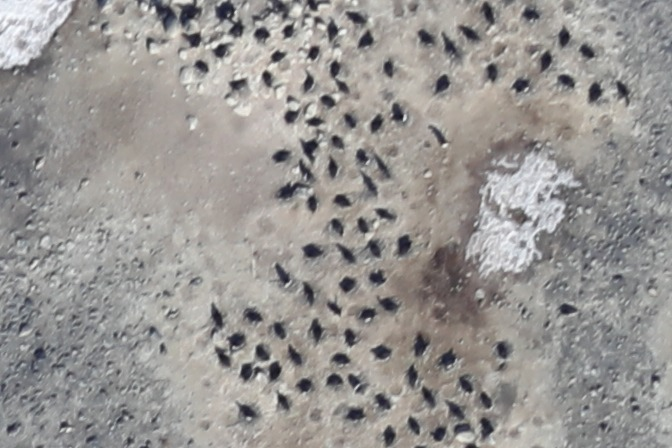
\includegraphics[width=0.475\linewidth]{figures/annotation/penguin/hallet.jpg}
  \caption{Cape Hallett 2017}
\end{subfigure}
\begin{subfigure}[t]{1.0\linewidth}
  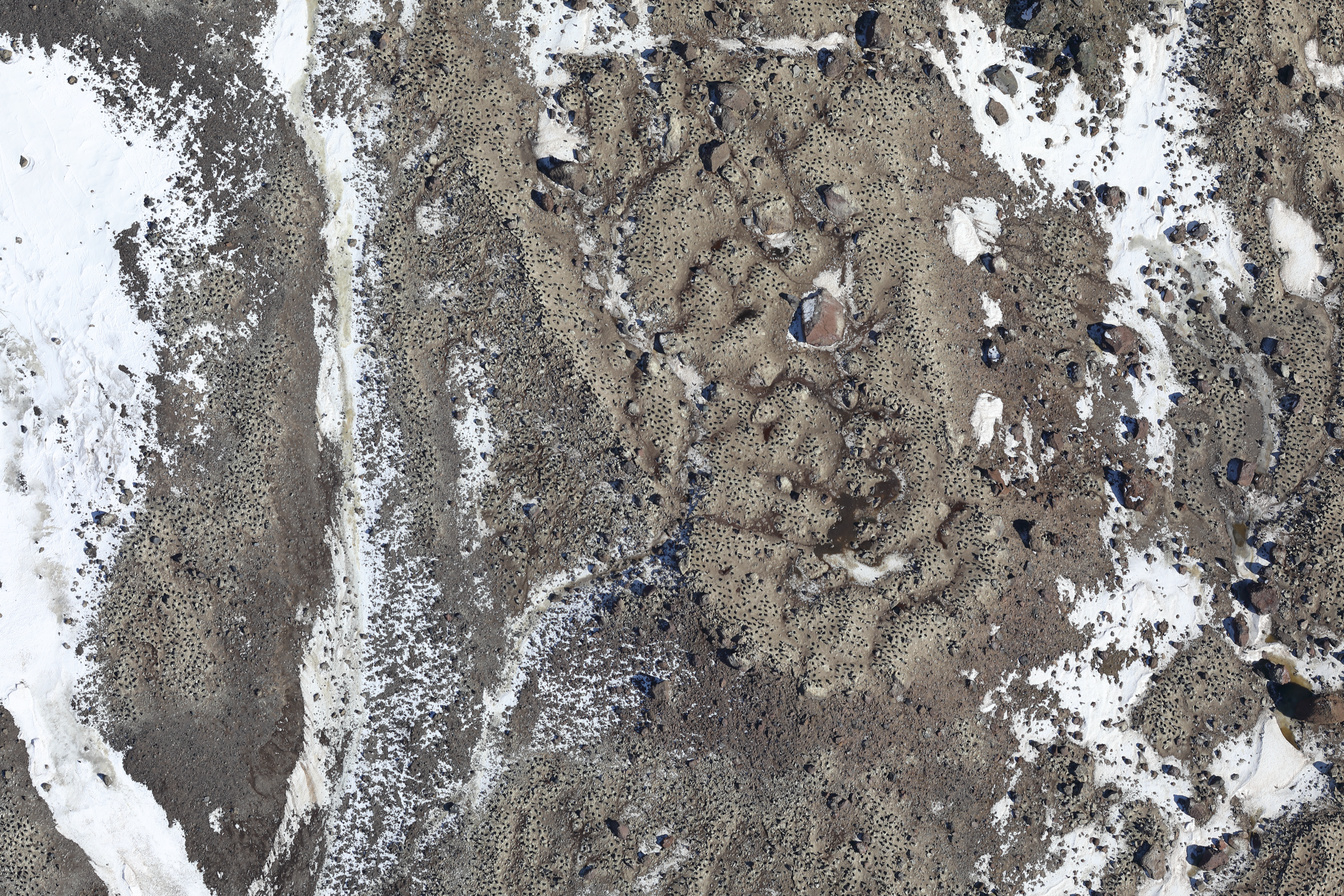
\includegraphics[width=0.475\linewidth]{figures/annotation/penguin/cotter_large.jpg}
  \hfill 
  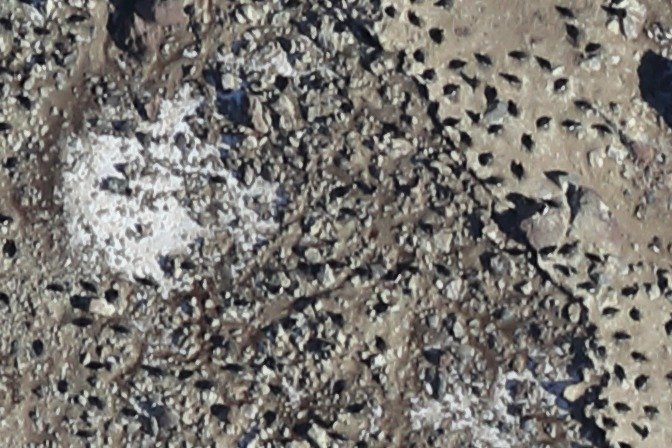
\includegraphics[width=0.475\linewidth]{figures/annotation/penguin/cotter.jpg}
  \caption{Cape Cotter 2017}
\end{subfigure}
\begin{subfigure}[t]{1.0\linewidth}
  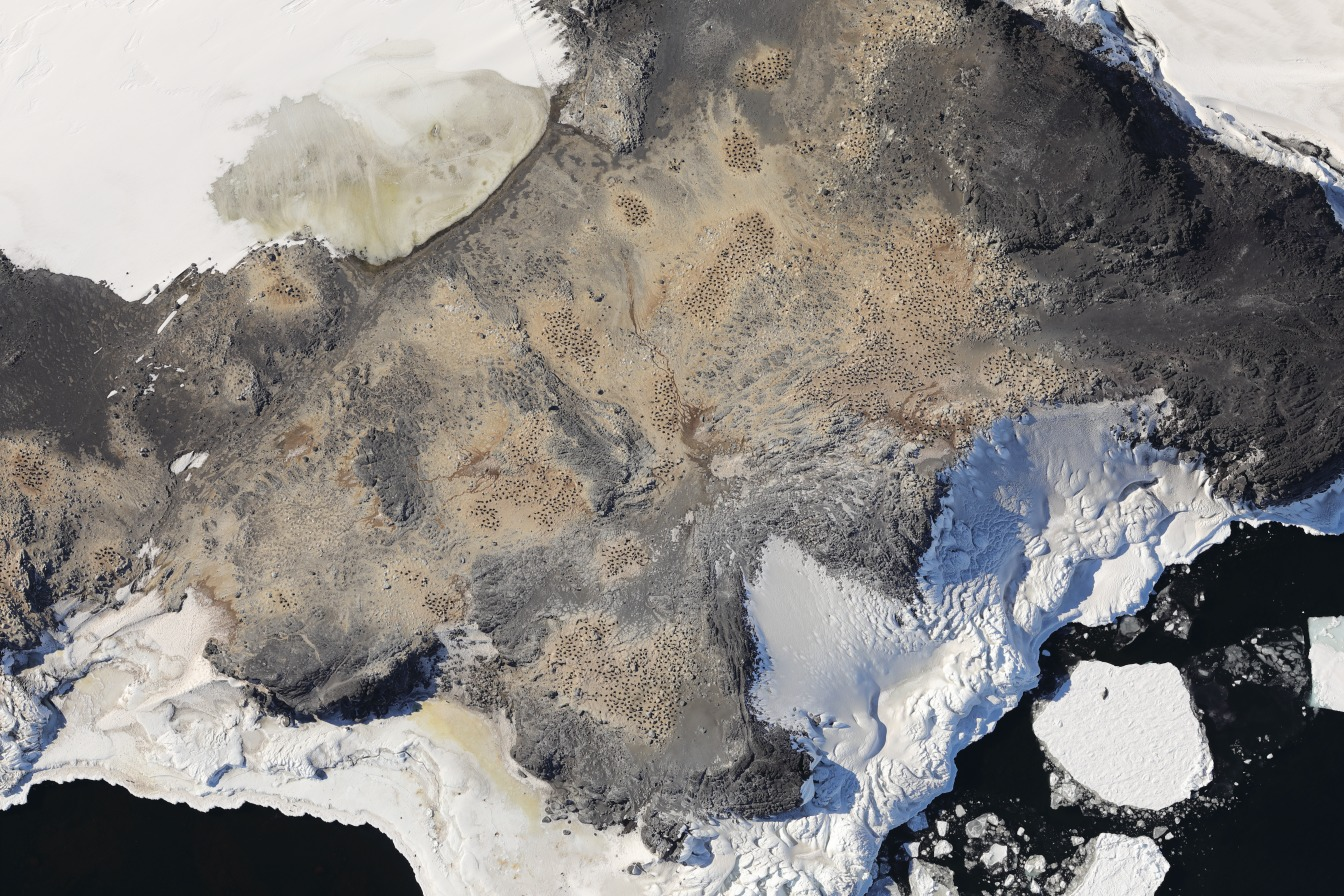
\includegraphics[width=0.475\linewidth]{figures/annotation/penguin/royds_large.jpg}
  \hfill
  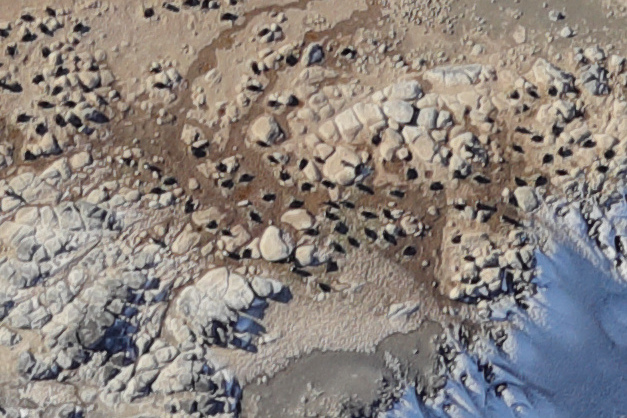
\includegraphics[width=0.475\linewidth]{figures/annotation/penguin/royds.jpg}
  \caption{Cape Royds 2017}
\end{subfigure}

\caption{Examples from the Ad\'elie penguin census data taken in 2017. On the left hand column are images showing the zoomed out landscape, on the right are representative crops zoomed in.  In (a) an image from Cape Hallet, showing clearly visible, easy to identify penguins as dark patches. In (b) Cape Cotter shows many more difficult to identify penguins, often with a high degree of ambiguity, not only for the machine learning algorithm but for a human annotator; rocky areas especially show shadows from rocks which are very difficult to discern from penguins. In (c) Cape Royds, a smaller colony to the other two (and complete) is, in terms of ambiguity and uncertainty, somewhere in between. }
\label {fig:penguin_examples}
\end{figure}


One task potentially useful for verification based annotation is counting things. It provides some of the time savings of automatic inference but also provides the accuracy of human annotation because the machine predictions are all verified. Additionally, counting can begin immediately on a new image set, without the first step of developing or training an object detector.

A source of inspiration for this work in verification based annotation came from \cite{McNeill2011}, where a tool was created to semi-automatically count Ad\'elie penguins from aerial photographs. The penguins are first automatically detected, then followed by a verification process allowing a human annotator to mark false positives and false negatives. Their method for detecting penguins is to first detect penguin colonies, which can often be done by the unique colour of the penguin guano. Individual penguins are then identified by thresholding, local minima detection, and then culling of long thin objects. 

The images (two of which can be seen in figure~\ref{fig:penguin_examples}), originate from aerial photographic surveys \cite{Lyver2014}, using high-resolution photographs, taken from 2000-2500 feet. In the case of the two images from Cape Cotter and Hallet in figure~\ref{fig:penguin_examples}, the images are cropped from images of size $ 6720\times4480 $. The Cape Royds images are spliced together from three images with various areas masked out, which was done by filling in the overlapping and irrelevant areas using a paint program.

The study has been conducted from 1981 until present, with manual counting of individual penguins prior to 2010. This involved manually counting individual penguins with a pin or marker used, to avoid duplication. 


\subsection {Method}

Separately, the three sets of penguins were counted using the annotation tool (each time beginning from scratch). Each set was annotated twice by different annotators (the second being the author) for the purpose  of comparing human consistency in annotation.

I used circle (centre and diameter) annotations to speed up the annotation process. For counting (especially at the resolution of individual penguins), the precise bounding box seems unnecessary, and is not needed to distinguish overlapping instances. For the same reason, the $AP_{50}$ metric is used, with the more relaxed \gls{IOU} matching threshold.

The very large original images were split into images of size $ 672\times448 $. Cape Royds images are slightly larger, but varying in size because the source images varied in size. Image crops of size $ 400\times400 $ were then used during training.

In the first counting, the count was impacted by a bug where the anchor centres were incorrect by a small amount, causing small localisation errors. Over time (and iteration of annotation and prediction), this had the undesirable effect of causing the circle centres to wander. In the second counting (counted by the author), this bug was fixed. Despite this problem impacting the trial, it also provides an opportunity to study the effect of providing noisy annotation localisation.

\subsection {Effect of image ambiguity}

One aspect, which can be studied from the penguin survey images, is how image based (aleatoric) uncertainty impacts the annotation process. It can be seen in figure~\ref{fig:penguin_examples} that between the three images from different geographical locations, each has a different level of uncertainty. Away from the rocky areas the penguins are clearly visible and easily distinguished, however those in rocky areas are often indistinguishable from shadows due to the blurry nature of the images at that scale.

When significant ambiguity is present in the source images (aleatoric uncertainty), a challenge is presented, not only for the object detector, but for the human annotator. Many of the penguin instances, to the untrained eye, appear very similar to the shadow cast by rocks and are difficult to discern. The nature of the imagery from the different sites shown in figure~\ref{fig:penguin_examples} provides a test case to compare the effectiveness of verification with different levels of uncertainty in the source image. 


\subsection{Results}
\label{sec:penguin_results}

\begin{table}[ht!]
  \centering
    \caption{Statistics from the three penguin sources. }
\begin{tabular}{llllll}
dataset     & counted & \shortstack{total  \\ minutes} & \shortstack{rate \\ (per minute)} & \shortstack {validation \\  $AP_{50}$} & \shortstack{percent \\ unmodified} \\
\toprule
$hallett$   & 4164    & 28.8          & 145               & 98.70     & 86.5\%   \\
$hallett_c$ & 4249    & 65.2          & 65.1              & 99.35     & 91.5\%   \\
$royds$     & 2783    & 30.7          & 90.6              & 88.73     & 88.1\%   \\
$royds_c$   & 2536    & 146           & 17.4              & 65.63     & 69.4\%   \\
$cotter$    & 6263    & 60.6          & 103               & 92.34     & 92.1\%   \\
$cotter_c$  & 6196    & 245           & 25.2              & 78.68     & 85.9\%  \\
\bottomrule
\end{tabular}

\label{tab:penguin_statistics}
\end{table}

The difference in degree of difficulty can clearly be seen in the difference of $AP_{50}$ in table~\ref{tab:penguin_statistics}, where the Cape Hallet penguins were detected with almost perfect accuracy, whereas the Cape Cotter penguins were more difficult, and those at Cape Royds were somewhere in between. 

The variation in model accuracy associated with the localisation bug can be clearly seen with especially \emph{cotter} and \emph{royds}, performing less well (although \emph{hallett} seemingly not suffering any ill effects). The two different people involved meant there were two different baselines, so direct comparison is not possible - but it can be seen that the model performance also contributes to significantly more user actions being required.


\subsubsection{Human consistency}

\begin{table}[h!]
    \centering
\caption{Comparison between human counters at very relaxed matching threshold $IoU >= 0.3$. }    
\begin{tabular}{lllll}
image set & $count$ & $count_c$ & matching & F1 score \\
\toprule
hallett   & 4164      & 4249      & 4105     & 0.98     \\
royds     & 2783      & 2536      & 2432     & 0.91     \\
cotter    & 6263      & 6196      & 5512     & 0.88 \\
\bottomrule
\end{tabular}
\label{tab:human_comparison} 
\end{table}
 
Despite difficulties, the actual counts are very similar between both people doing the counts, seen in table~\ref{tab:human_comparison}. Images from Cape Hallett, as well as being easy to detect for an object detector, are also unambiguous to a human annotator, and both counts match closely. Both \emph{royds} and \emph{cotter} have significantly less overlap between matched human counts, although the raw numbers are still quite similar.

A very low threshold was used ($IoU >= 0.3$) for matching between human counts, because some systematic differences were present regarding where the penguin was marked on the image.

\subsubsection {Counting rate}

\begin{figure}[ht]
\centering
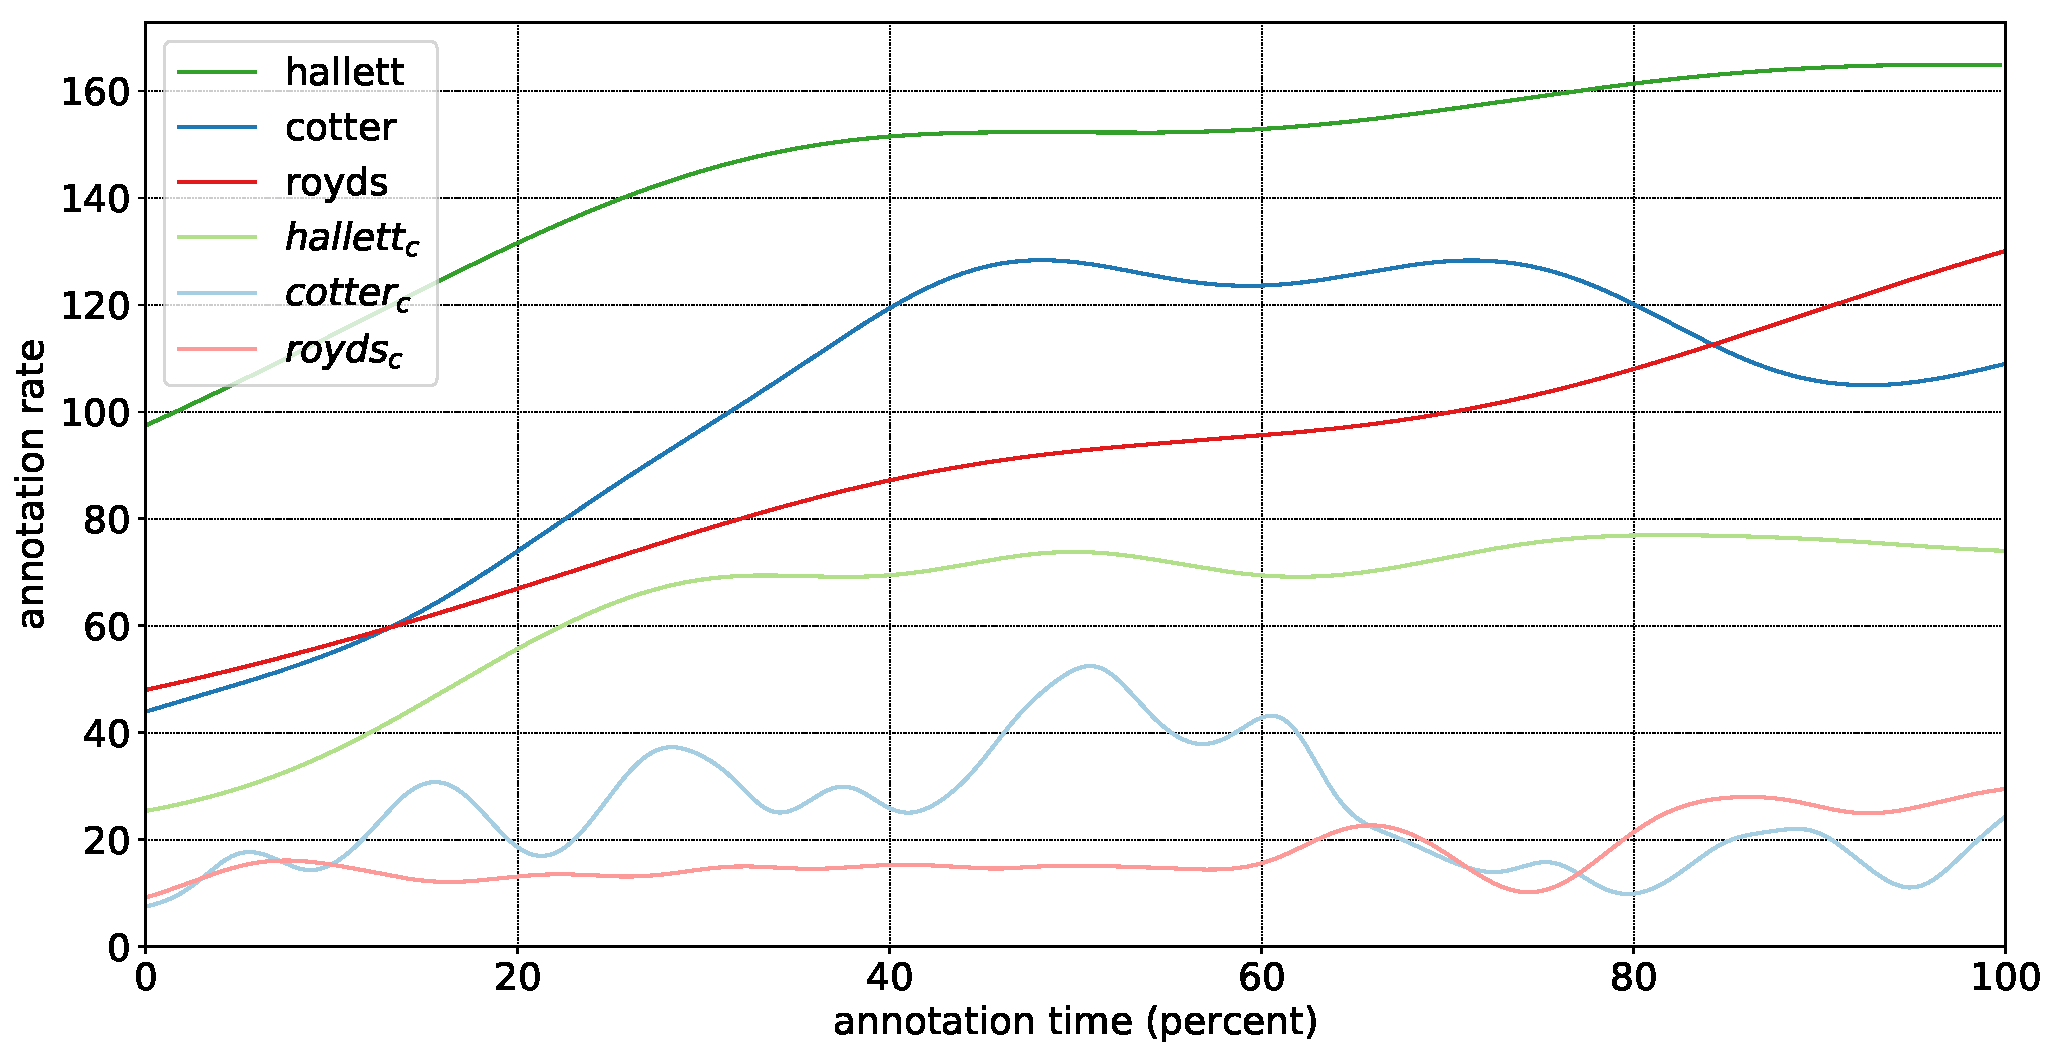
\includegraphics[width=1.0\linewidth]{charts/aerial_penguins/summaries/instance_rates.pdf}
\caption{ Rates of counting for the three different image subsets, for both counting runs }
\label{fig:penguin_rates}
\end{figure}

\begin{figure}[ht]
\centering
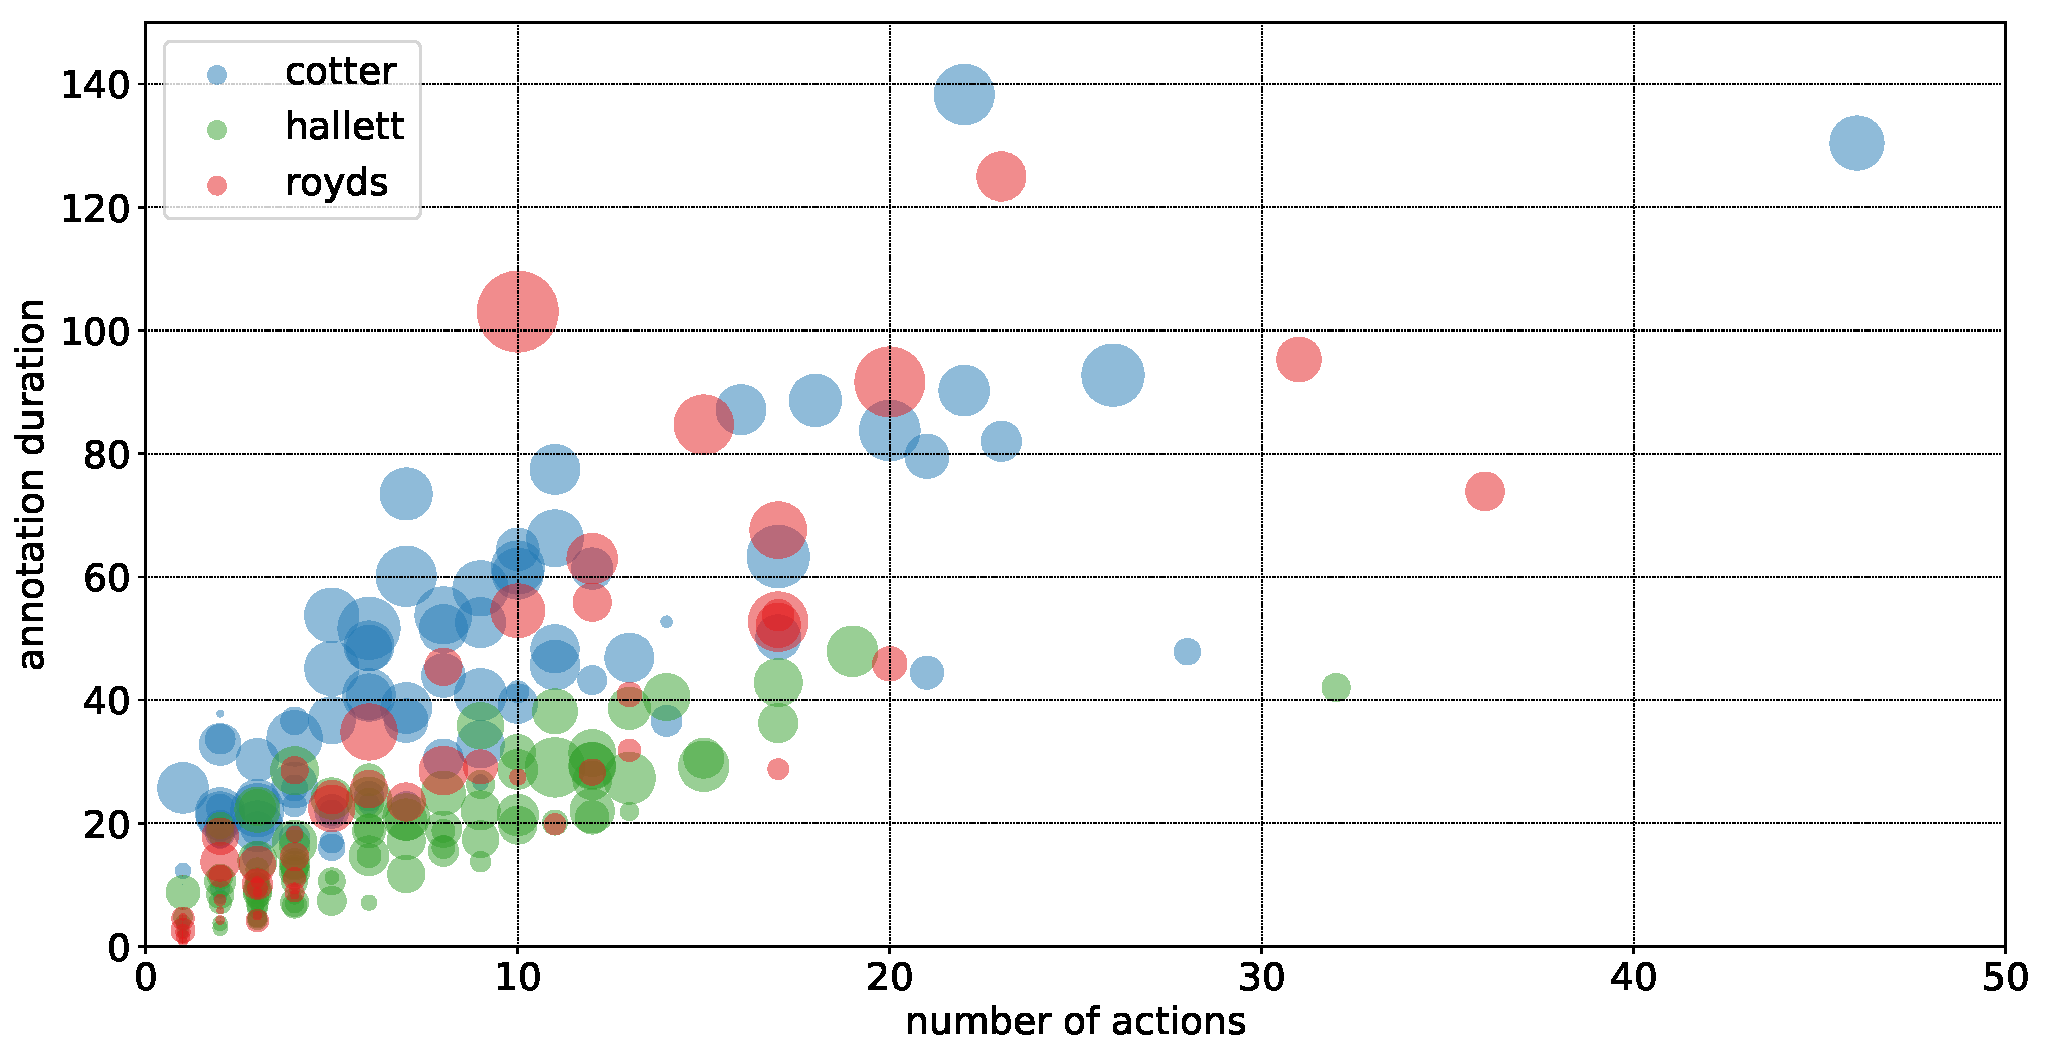
\includegraphics[width=1.0\linewidth]{charts/aerial_penguins/actions_time_a.pdf}
\caption{ Number of actions vs. counting duration for each image between image subsets; the area of each point is proportional to the number of instances counted }
\label{fig:actions_time_penguins}
\end{figure}


\subsubsection{Limitations and confounding factors}

Aside from the localisation bug affecting the first counting trial, there were other issues which impacted on the practicalities of  counting, such as the following:

\begin{itemize}
    \item {\textbf{Cropping boundaries}}\par
Penguins tend to nest in groups. This meant that cropping images neatly at regular sizes from the large input images would quite often crop regions with a small part of a group along the edge. To recognise an individual penguin, or differentiate it from the shadow of a rock, the context is important. A difficult ambiguous black blob would much more likely be a penguin if it was part of a larger group, yet on its own it would be much more likely to be a rock. A method of dividing images which showed more context, for example overlapping crops, would make counting easier.
    \item {\textbf{Number of objects}}\par
Despite the smaller crop sizes used, the number of penguins in each image is much larger than other datasets the tool had previously been tested on. It was found that the performance of the \gls{SVG} based interface implementation lagged noticeably and impaired usability on images that had larger numbers of penguins. 
    \item {\textbf{Annotations obscuring the image}}\par
Due to the ambiguity in some images and the size of the penguins,  the annotation markers sometimes obscure the image, making it harder to differentiate between shadows and penguins. It was noticed during the first counting run that the user was dragging annotations around in order to see more effectively. An improvement would be to provide a toggle to hide annotations, or use a higher threshold so that less effort was needed to check for false positives.

\end{itemize}


\subsection{Conclusion}
\label{sec:penguin_conclusion}

Verified counting, using tools intended for annotation seems promising. In the small scale trials presented here, counting rates can be seen in some cases to be higher than should be possible, with manual counting reaching rates of $145$ per minute for the Cape Hallet penguins, which are visually very distinct, and slightly less for more uncertain imagery from Cape Royds and Cape Cotter. From the point of view of the best quality automated counting, improved resolution in the images would make the task much easier. 

The bug in localisation, which occurred in the first counting trial, served to demonstrate the problems which can arise from poor localisation accuracy on the part of the object detector. Even so, the two counting trials produced similar counts, especially for the very certain images of Cape Hallett and showed that, like object detection algorithms, human verified counts are also more variable for uncertain images. Several practical problems can be addressed in future work, after which, larger scale counting trials (over larger colonies or whole years) would be a logical step.

\subsection{Case Study: Time series Waddell seal counts}
\label{sec:case_seals}



\begin{figure}[ht!]
\centering
\begin{subfigure}[t]{1.0\linewidth}
  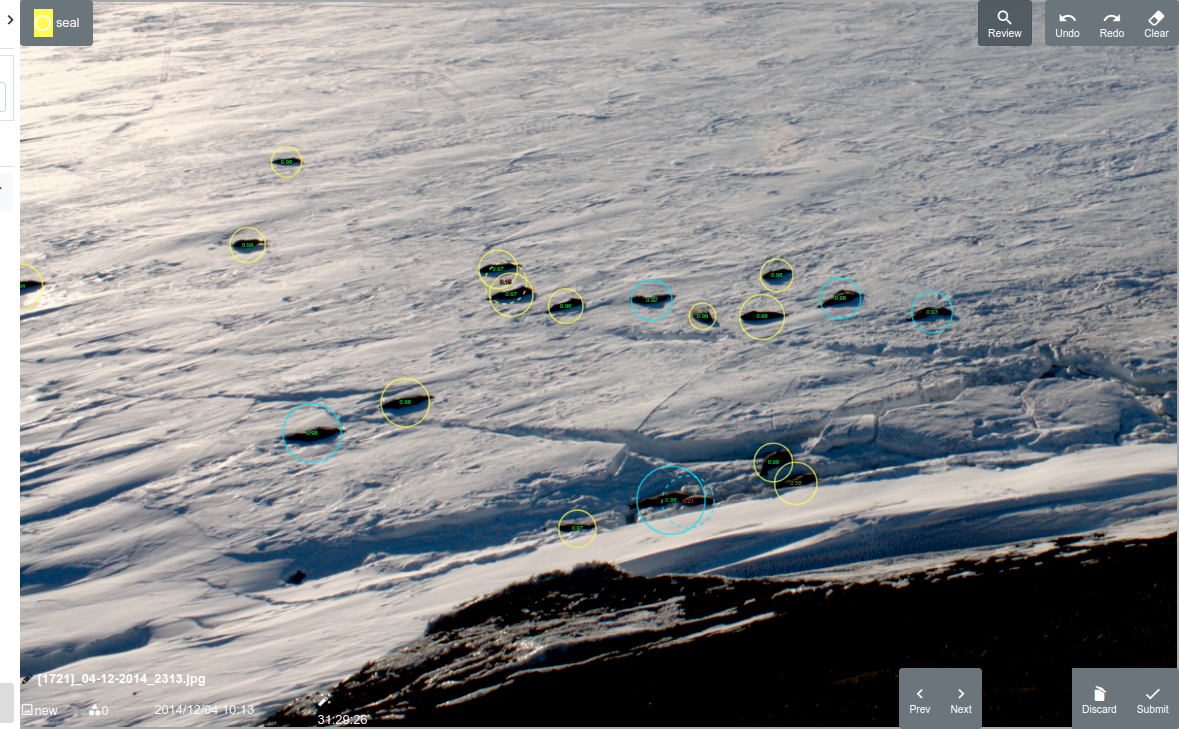
\includegraphics[width=0.475\linewidth]{figures/annotation/screenshots/seals_small2.png}
  \hfill
  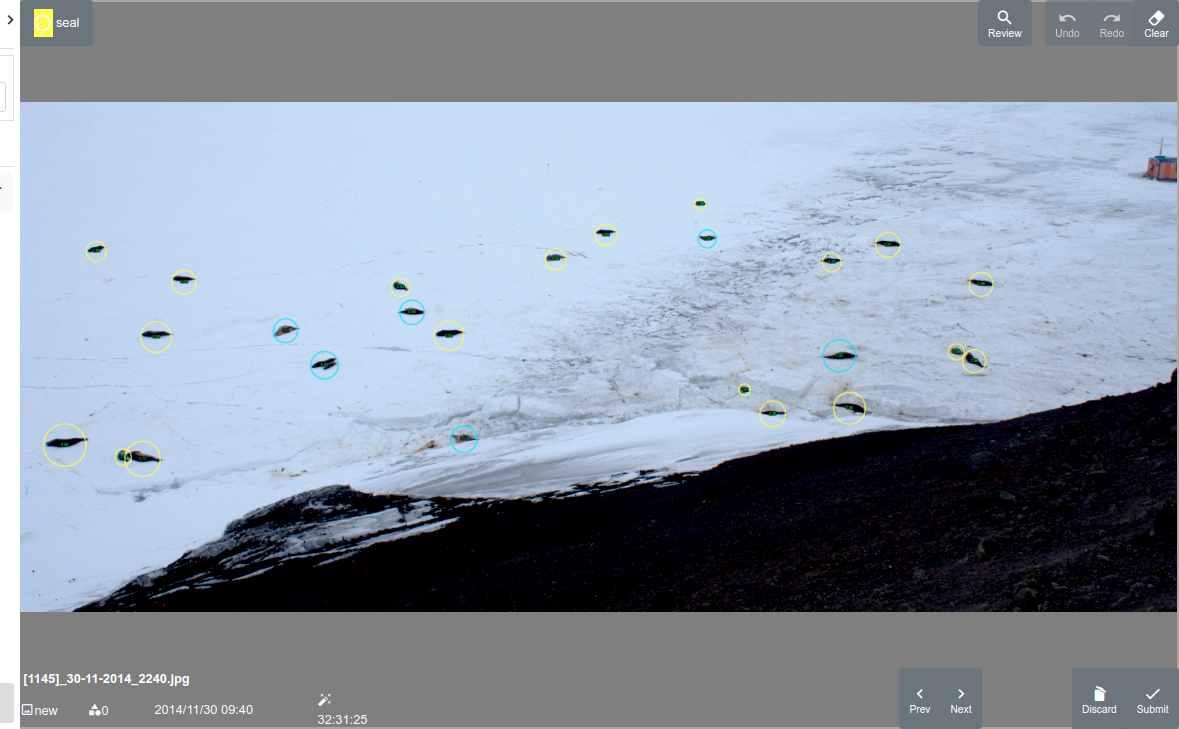
\includegraphics[width=0.475\linewidth]{figures/annotation/screenshots/seals_small.png}
  \caption{}
\end{subfigure}

\begin{subfigure}[t]{1.0\linewidth}
  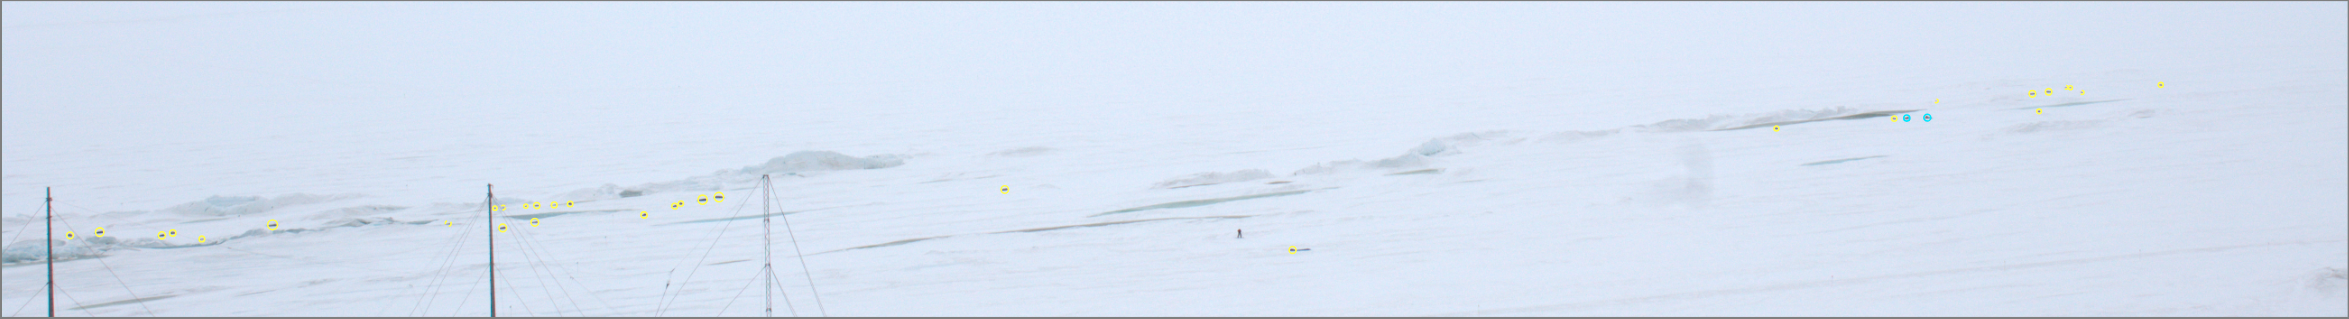
\includegraphics[width=1.0\linewidth]{figures/annotation/screenshots/cam_c.png}
\end{subfigure}

\begin{subfigure}[t]{1.0\linewidth}
  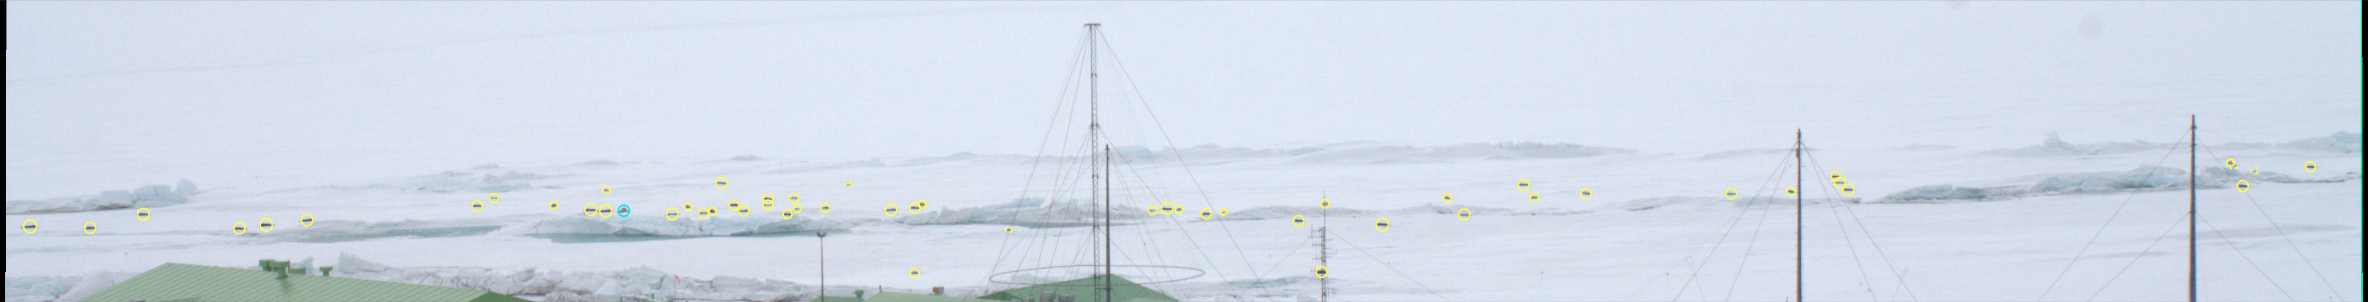
\includegraphics[width=1.0\linewidth]{figures/annotation/screenshots/cam_b.png}
  \caption{}
\end{subfigure}


\caption{ Images from (a) the Turtle Rock (\emph{seals}) image set, and (b) full images from Scott Base (\emph{scott base}) showing the wide angle crop used.  }
\label {fig:weddell_images}
\end{figure}


Here I examine the two time series image sets in more depth: (a) \emph{seals}  \cite{Eisert2015}, images captured at Turtle Rock and (b) \emph{scott base}  \cite{Eisert2019}, images captured from a viewpoint on a hill overlooking Scott Base. The images were captured from fixed cameras at 10 minute intervals for the purpose of monitoring both Weddell seal populations (\emph{scott base}) and haul-out patterns (\emph{seals}) to avoid predation. 


\subsection{Turtle Rock \cite{Eisert2015}}
 
 Images from Turtle Rock were previously counted using the crowd sourcing platform Zooniverse \cite{Zooniverse}, where seals were counted by placing point markers. This work is part of a larger work comparing crowd sourcing with \gls{CNN} object detection based approaches, for Antarctic population monitoring. 
 
 Figure~\ref{fig:zooniverse_counts} shows the original counting using crowd sourced counting on the Zooniverse \cite{Zooniverse} platform. Each point is a users count for an image. Users of this system mark seal locations with a point in order to count them. A major motivator for using a \gls{CNN} object detector was the source of noisiness apparent in the crowd source counting. One potential advantage over crowd sourced based counting is the consistency which can come from having one person annotate images, as well as the predictions from the object detector; a potential disadvantage is the risk that algorithmic bias is introduced.
 
 The images were counted twice by annotating a subset of images and extrapolating counts using the trained object detector. Dataset $seals_b$ was annotated by an expert in antarctic wildlife and the dataset $seals$ was annotated by the author, who during the development of the tool also had considerable practice. 
 
 The major challenge in annotation (and for the trained object detector) was identifying mothers with pups compared to those without. Often the pup would be mostly (or fully) obscured.  Due to the rapid growth rate, the pups would grow from birth to almost adult size over the observation period. Other difficulties were occasional harsh lighting and dying or dead seals, and the difficulty of when to include or exclude them in the count.

 
\begin{figure}[pht!]
    \centering
    
    \begin{subfigure}[t]{1.0\linewidth}
    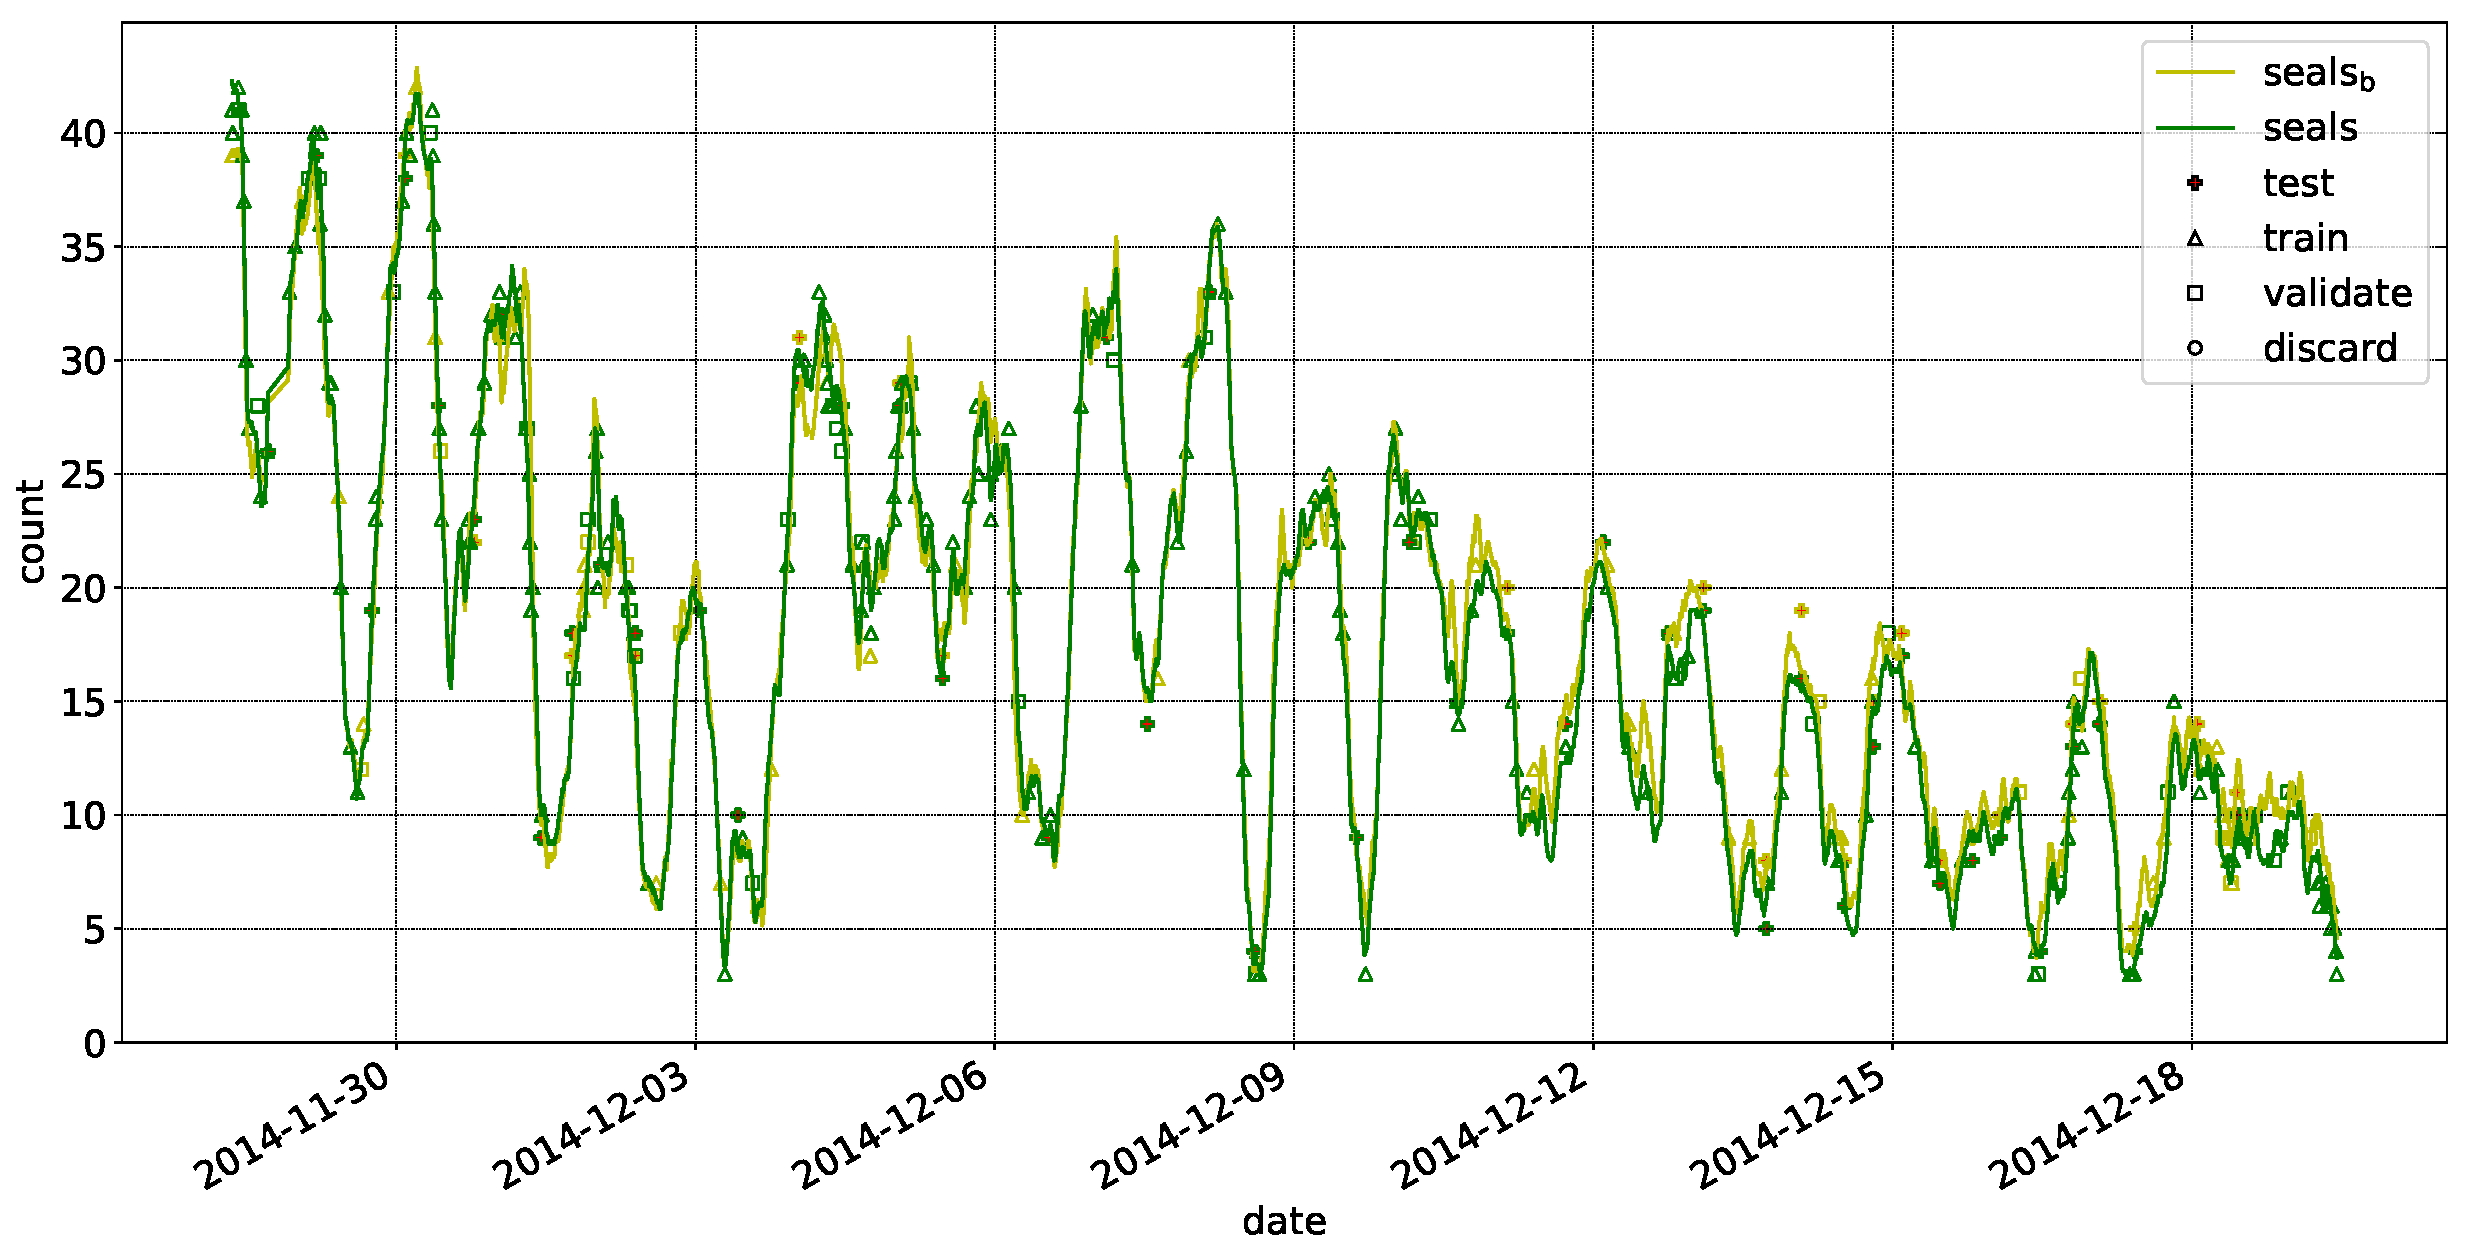
\includegraphics[width=1.0\linewidth]{charts/seals/seals_combined.pdf}
    \caption{Estimated counts (solid lines) along with images counted by annotation using the \gls{VBA} tool (shown as points). Two separate countings are shown, both $seals$ and $seals_b$, where annotated images, which are a different random subset in each case (shown split into two parts: \emph{train} and \emph{validate}). The two countings of the test set of 46 images are also shown. }
    \label{fig:turtle_rock}
    \end{subfigure}
    
    
    \begin{subfigure}[t]{1.0\linewidth}
    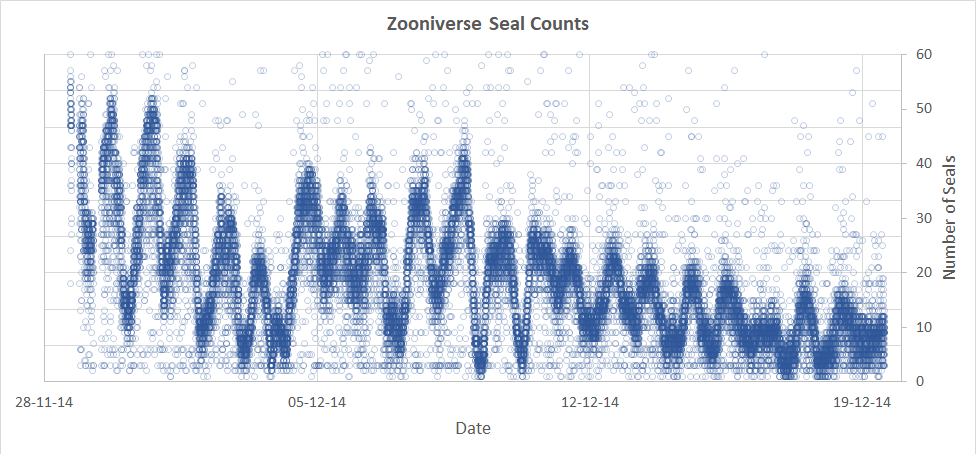
\includegraphics[width=1.0\linewidth]{figures/annotation/zooniverse.png}
    \caption{Raw counts from crowd sourced counting on the Zooniverse \cite{Zooniverse} platform, each image is counted 12 times. \cite{Eisert2017}}
    \label{fig:zooniverse_counts}
    \end{subfigure}
    
    \caption{}
    \label{fig:seals_timeseries}
\end{figure} 




\subsubsection{Test sets}

In order to make comparisons between human annotators and automated counts from the object detector, a set of 46 images were selected. This set of 46 images were then carefully annotated by both human annotators and then set aside for testing. A second annotation was then performed, using the set of test images for comparing accuracy with the machine counts. The test image counts can be seen in figure~\ref{fig:turtle_rock} where they're plotted with markers in red. 

% Average differences between the human counted test sets and machine counts on the same images is seen in figure~\ref{fig:test_comparison} where the differences between human counts 

% \begin{table}[h!]
%     \centering
% \caption{Average counting error between images, human counted test sets and machine counts on the same images for two different training sets.}    
% \begin{tabular}{lllll}
%  & $human_a$ & $estimate_a$ & $human_b$ & $estimate_b$ \\
% \toprule
% $human_a$        &  0.0   &   $0.63\pm0.76$    &  $0.67\pm0.81$     &  $1.28\pm1.22$   \\
% $estimate_a$     &       &    0.0   & $ 1.0\pm0.    &   1.40   \\
% $human_b$        &       &       &    0.0  &    1.22   \\
% $estimate_b$     &       &       &      &     0.0  \\
% \bottomrule
% \end{tabular}
% \label{tab:test_comparison} 
% \end{table}




\subsection{Scott Base \cite{Eisert2019}}

\begin{figure}[ht]
    \centering
    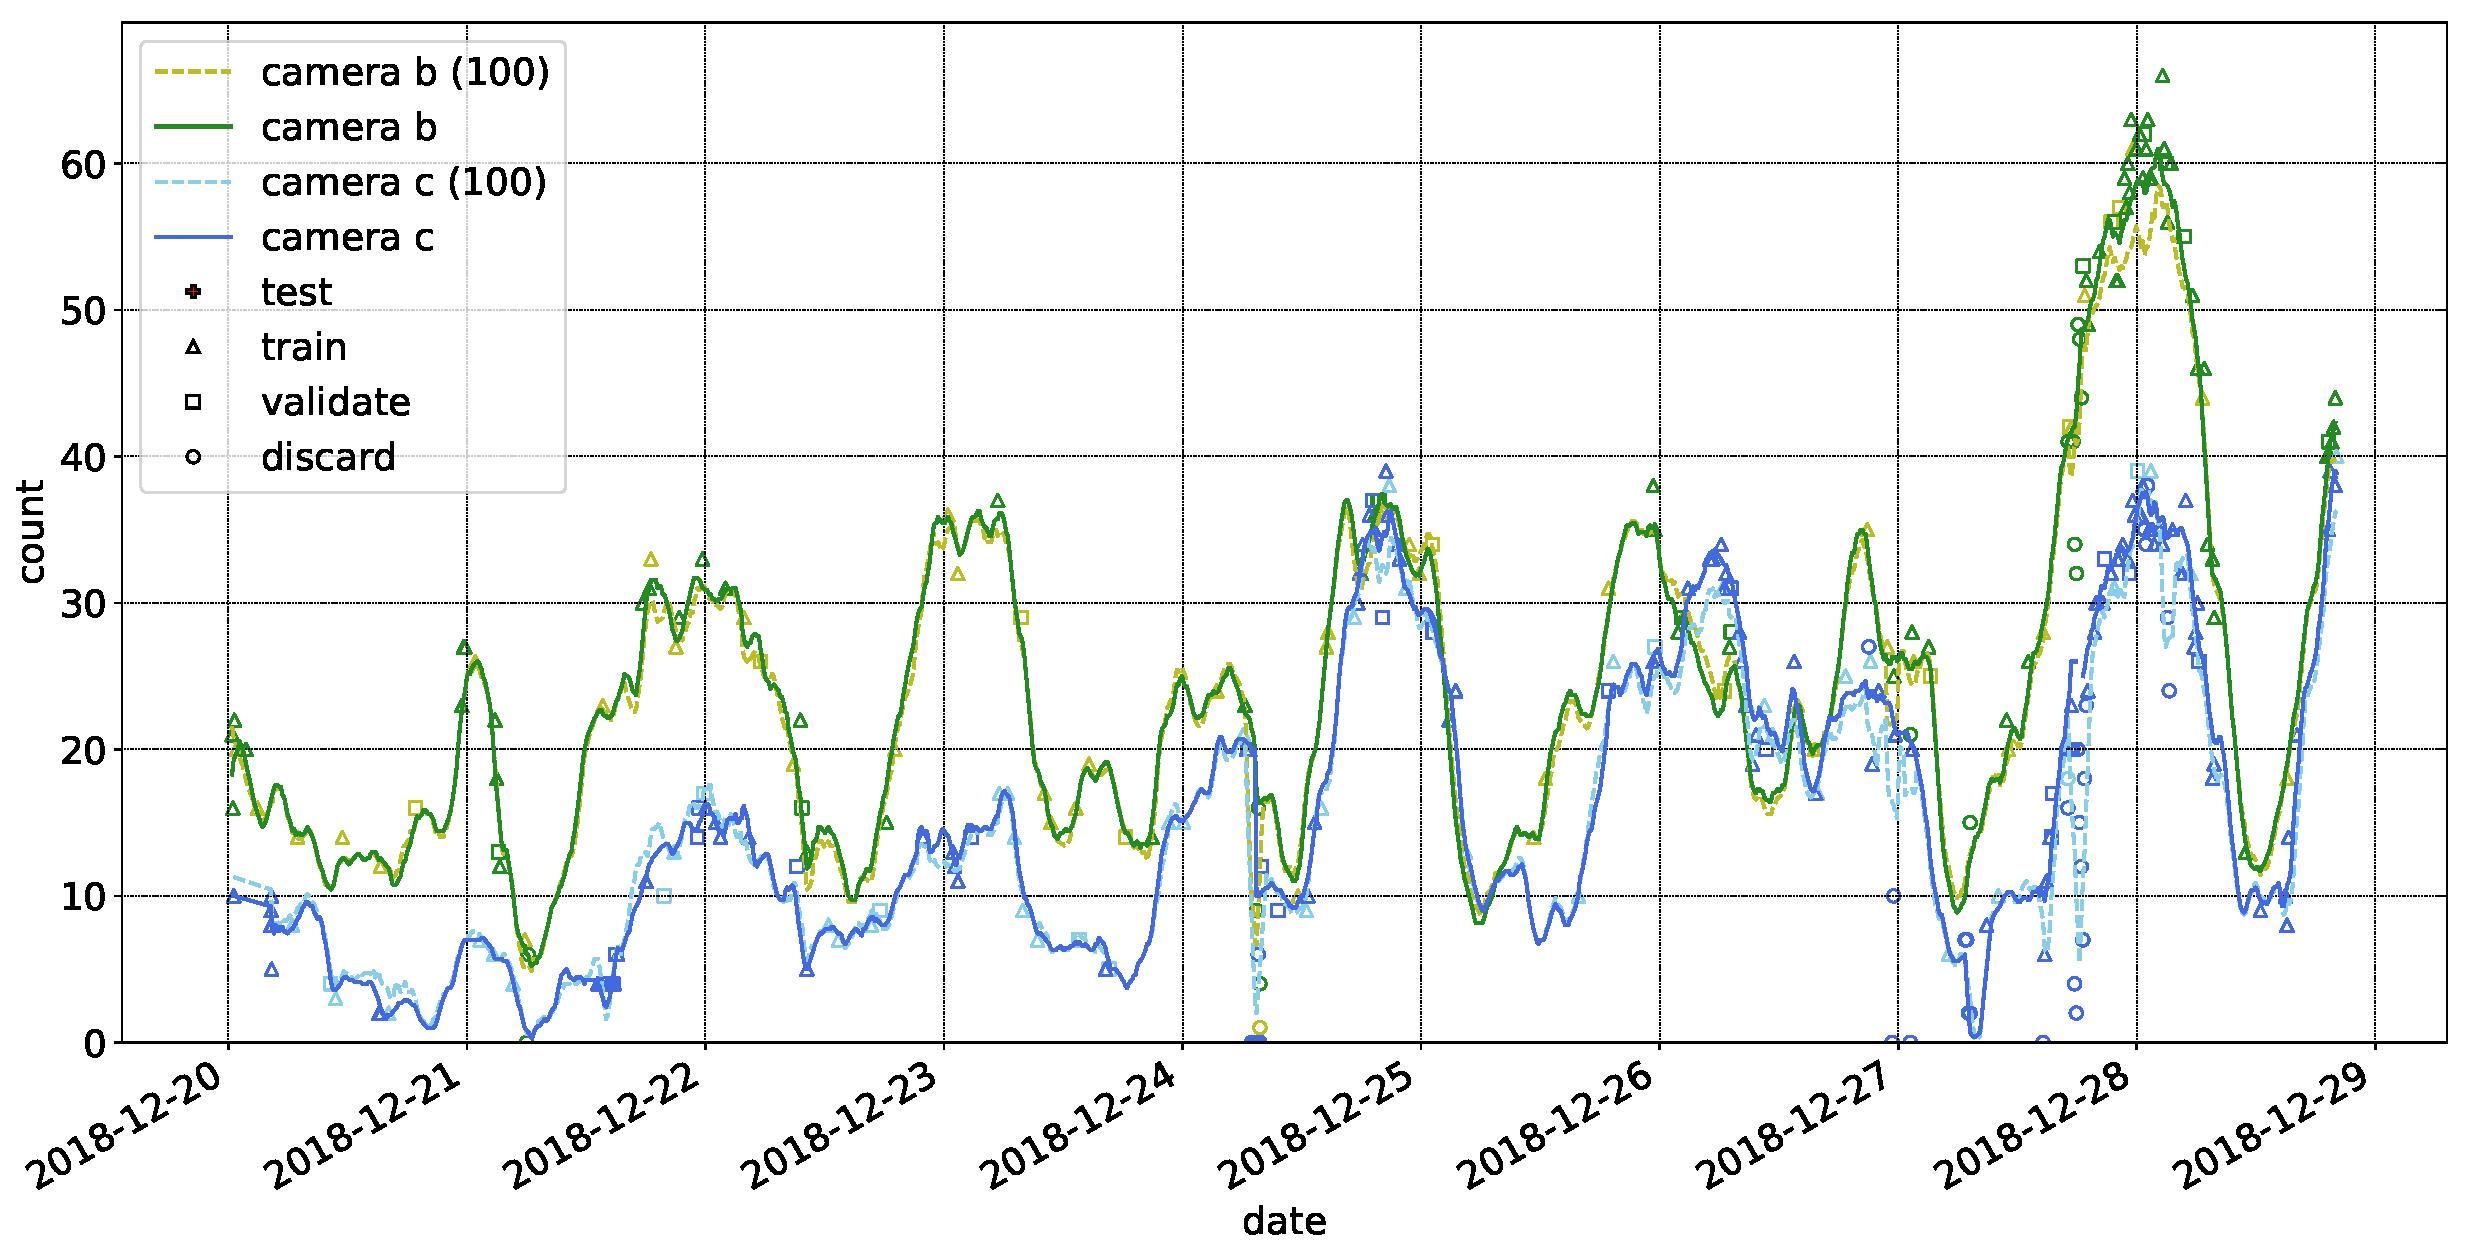
\includegraphics[width=1.0\linewidth]{charts/seals/scott_base_combined.pdf}
    \caption{Estimated counts (solid lines) along with images counted by annotation using the \gls{VBA} tool (shown as points). Counts for two different viewpoints are shown. Dotted lines for each viewport show the progress after annotating 100 randomly sampled images, solid lines show the full count after 301 images, with the last 201 images selected using frame consistency as a heuristic to attempt to eliminate outliers. Discontinuity on lines shows sections with discarded images due to poor visibility from inclement weather. }
    \label{fig:scott_base}
\end{figure}
